\documentclass[12pt,oneside,reqno,a4paper,twoside]{report}
\usepackage[utf8]{inputenc}
\usepackage{amsmath,amsthm}     % ams stuff should be before font loading
\usepackage{lmodern}
\usepackage[T1]{fontenc}        % should be after font loading
\usepackage{babel}
\usepackage[numbers]{natbib}    % bibtex package
%\usepackage{typearea}           % custom type area
%   \areaset[0mm]{135mm}{210mm}  % typearea configuration
%   \topmargin5mm                % typearea configuration
\usepackage{graphicx}
\usepackage{url}
\usepackage{tocloft}
%\usepackage{verbatim}
\usepackage{forest}
\usepackage{float}

%Added the below two lines for adding chapter number in images
\usepackage{chngcntr}
\counterwithin{figure}{section}

\usepackage{ifpdf}
\ifpdf
  \pdfminorversion=5
  \pdfoutput=1
% Diese Pakete laufen anscheinend nur mit pdflatex gescheit
    \usepackage[bitstream-charter]{mathdesign}
    \usepackage[pdfusetitle,colorlinks=true,linktoc=all]{hyperref}
\else
    \usepackage{times}
    \usepackage[dvips,ps2pdf,linktoc=all]{hyperref}

\fi

\ifdefined\hypersetup
  \hypersetup{
    pdfkeywords={}, linkcolor=black, citecolor=black, filecolor=black, urlcolor=black,
  }
\fi

%Load additional packages
\usepackage[utf8]{inputenc}

% Load the required packages
%\usepackage[binary-units,abbreviations]{siunitx}
\usepackage[abbreviations, shortcuts=true]{glossaries-extra}

% Set the abbreviation style
\setabbreviationstyle{long-short}

% Include the abbreviations file
\newabbreviation{pcb}{PCB}{Printed Circuit Board}
\newabbreviation{fc}{FC}{Fully Connected}
\newabbreviation{ng}{NG}{Not Good}
\newabbreviation{gpu}{GPU}{Graphics Processing Unit}
\newabbreviation{cpu}{CPU}{Central Processing Unit}
\newabbreviation{tpu}{TPU}{Tensor Processing Unit}
\newabbreviation{ipu}{IPU}{Intelligence Processing unit}
\newabbreviation{resnet}{ResNet}{Residual Neural Network}
\newabbreviation{auroc}{AUROC}{Area Under the Receiver-Operating Curve}
\newabbreviation{aupr}{AUPR}{Area Under the Precision-Recall Curve}
\newabbreviation{dl}{DL}{Deep Learning}
\newabbreviation{cv}{CV}{Computer Vision}
\newabbreviation{tpr}{TPR}{True Positive Rate}
\newabbreviation{fpr}{FPR}{False Positive Rate}
\newabbreviation{tp}{TP}{True Positive}
\newabbreviation{fp}{FP}{False Positive}
\newabbreviation{tn}{TN}{True Negative}
\newabbreviation{fn}{FN}{False Negative}
\newabbreviation{svm}{SVM}{Support Vector Machine}
\newabbreviation{k-nn}{K-NN}{k-Nearest Neighbors}
\newabbreviation{cnn}{CNN}{Convolutional Neural Network}
\newabbreviation{yolo}{YOLO}{You Only Look Once}
\newabbreviation{vae}{VAE}{Variational Auto-Encoder}
\newabbreviation{gan}{GAN}{Generative Adversarial Network}
\newabbreviation{dfm}{DFM}{Deep Feature Modeling}
\newabbreviation{dnn}{DNN}{Deep Neural Networks}
\newabbreviation{pca}{PCA}{Principal Component Analysis}
\newabbreviation{t-sne}{t-SNE}{t-Distributed Stochastic Neighbor Embedding}
\newabbreviation{gmm}{GMM}{Gaussian Mixture Models}
\newabbreviation{kde}{KDE}{Kernel Density Estimation}
\newabbreviation{pdn}{PDN}{Patch Description Network}
\newabbreviation{s-t}{S-T}{student-teacher}
\newabbreviation{vit}{ViT}{Vision Transformer}
\newabbreviation{auc}{AUC}{Area Under the Curve}
\newabbreviation{dfkde}{DFKDE}{Deep Feature Kernel Density Estimation}
\newabbreviation{ann}{ANN}{Artificial Neural Networks}
\newabbreviation{fnn}{FNN}{Feed Forward Neural Networks}
\newabbreviation{relu}{ReLu}{Rectified Linear Unit}
\newabbreviation{iou}{IOU}{Intersection Over Union}
\newabbreviation{fpn}{FPN}{Feature Pyramid Network}
\newabbreviation{pan}{PAN}{Path Aggregation Network}
\newabbreviation{nll}{NLL}{Negative Log-Likelihood}
\newabbreviation{fre}{FRE}{Frequentist}
\newabbreviation{deit}{DeiT}{Data-Efficient Image transformer}
\newabbreviation{cait}{CaiT}{Class-Attention in Image Transformer}
\newabbreviation{aoi}{AOI}{Automated Optical Inspection}
\newabbreviation{nlp}{NLP}{Natural Language Processing}
\newabbreviation{mlp}{MLP}{Multi-Layer Perceptron}
\newabbreviation{msa}{MSA}{Multiheaded Self-Attention}
\newabbreviation{ln}{LN}{Layer Normalization}

	
\usepackage{blindtext}

\usepackage{fancyhdr}

% Das ist nur fuer den Blindtext zustaending


% Blattlayout
\textwidth15cm
\textheight23cm
\topmargin0cm
\oddsidemargin0.5cm
\evensidemargin0.5cm

% Adjust header height as per the warning
\setlength{\headheight}{14.49998pt}
\addtolength{\topmargin}{-2.49998pt}

% Einzug f"ur den Absatz
\parindent0em
\parskip0.5em
% Header, Footer
\usepackage{fancyhdr}
 % Text in Kopfzeile aussen
\fancyhead[LE,RO]{\nouppercase{\leftmark} }
% Text in Kopfzeile innen
\fancyhead[RE,LO]{}
% Text in Fusszeile mittig
\fancyfoot[CE,CO]{\thepage}
\pagestyle{fancy}

\begin{document}

\pagenumbering{Alpha}
\renewcommand{\thepage}{C-\Roman{page}}
\begin{titlepage}
      \textsf{
    \begin{center}
      %\vspace*{1cm}
    \huge \textbf{Solder Inspection for Pseudo Error Reduction in Printed Circuit Board production using Unsupervised Learning} \\%TODO
    \vspace{2cm}
    \LARGE\textbf{Master's Thesis}\\[5mm]
    \Large for the degree of \\[5mm]
    \textbf{Master of Science (M.Sc.) \\[5mm]
    Data Science\\[5mm]
    %TODO Mathematics\\[5mm]
    %TODO Mathematical Economics\\[5mm]
    %TODO Data Sience\\[5mm]
    %TODO Computational and Applied Mathematics \\[5mm]
    }
    at the Faculty of Sciences of\\ Friedrich-Alexander-Universität
    Erlangen-Nürnberg\\[1cm]
    in Cooperation with\\ Siemens AG, Berlin, Germany\\[1cm]
    submitted on 22-10-2024 \\[3mm] %TODO
    by \textbf{Rohit Potdukhe} %TODO
    \vfill
    \normalsize
    Advisor: Prof. Dr. Enrique Zuazua\\Supervisor: Dr. Majid Mortazavi
    \\[3em] %TODO
    
\includegraphics[width=0.5\textwidth]{logo/fau-nat-digital}
    \end{center}
%
}
\end{titlepage}

\pagenumbering{Roman}

\begin{center}
    Ich versichere, dass ich die Arbeit ohne fremde Hilfe und ohne Benutzung anderer als der angegebenen Quellen angefertigt habe und dass die Arbeit in gleicher oder ähnlicher Form noch keiner anderen Prüfungsbehörde vorgelegen hat und von dieser als Teil einer Prüfungsleistung angenommen wurde. Alle Ausführungen, die wörtlich oder sinngemäß übernommen wurden, sind als solche gekennzeichnet.
\end{center}

\newpage 

\textbf{Non-disclosure notice}


The Academic Work contains confidential information that is subject to secrecy. Therefore, the Academic Work must not be duplicated or published without prior written approval of Siemens AG.\\\\\\\\\\


\textbf{Sperrvermerk}


Die Arbeit beinhaltet vertrauliche Informationen, die der Geheimhaltun unterliegen. Aus diesem Grund darf die Arbeit ohne vorherige schriftliche Zustimmung der Siemens AG nicht vervielfältigt oder veröffentlicht werden.

\newpage
\begin{center}
    \section*{Acknowledgements}
\end{center}
\sloppy
First and foremost, I would like to thank my supervisor, Dr. Majid Mortazavi, for his invaluable guidance, support, and encouragement throughout the course of my research. His insights and expertise were crucial to the successful completion of this work.
I am also deeply grateful to my advisor, Prof. Dr. Enrique Zuazua, for his continuous support, constructive feedback, and for always being available to discuss ideas and provide guidance.
I would like to extend my gratitude to Siemens AG, Berlin, Germany, for providing me with the opportunity to conduct my research in collaboration with their team and for providing me with the required resources.
Finally my heartfelt thanks go to my family and friends for their unwavering support, patience, and understanding throughout this journey. Their encouragement has been a source of strength for me.

\newpage % To ensure the abstract starts on a new page

% Abstract
%\begin{abstract}
%\end{abstract}

\begin{center}
\bfseries
% Abstract in English
{\selectlanguage{english}Abstract}
\normalfont
\end{center}
\sloppy
The inspection of the solder joint in the manufacturing of printed circuit boards (PCBs), ensures the quality and reliability of the product. Traditionally, it is done by manual examination or by training a supervised machine learning model where an expert is used to label the dataset manually. This dependency on labeled data forms a bottleneck in efficiency and, hence, scaling in production. As PCB designs become more complex and the demand for shorter production cycles intensifies, innovative inspection methods must be developed to detect solder-joint defects without using an extensive prelabeled dataset.
Our research addresses this challenge using unsupervised learning techniques for solder joint defect detection. We have leveraged the Anomalib library, a comprehensive collection of a wide range of anomaly detection algorithms, to implement and evaluate multiple models like PatchCore and DFM, among others. Our approach involves training or inferencing using these models on an image dataset of solder joints. The models then label the solder joints as normal or abnormal, with a corresponding prediction score for each image. This, therefore, removes the need for a manually labeled training dataset and can be more scalable and adaptable for inspection requirements on PCBs. The PatchCore model provided very promising results, showing an accuracy of 91.25\%.
During the course of the thesis, we encountered few challenges that provided us with a lot of information regarding the practical application of these techniques. The most prominent ones are related to significant training times for some models, which may hinder their feasibility in real-time manufacturing environments. Looking towards future developments, a more extensive use of Vision Transformers will bring huge potential to this application. Although some ViT models are explored in our current work to some extent, there is much space for a more elaborate exploration of their potential in unsupervised defect detection. Further efforts could thus be oriented toward developing such models, optimized for faster training and inferencing times, and investigating their generalization capability for different solder joint defects.




\clearpage

% Set the dots for the sections
\renewcommand{\cftsecleader}{\cftdotfill{\cftdotsep}}
\tableofcontents

\clearpage \pagenumbering{arabic}

\section{Introduction}
\label{sec:introduction}

Intro will come here

\begin{figure}[ht!]
    \centering
    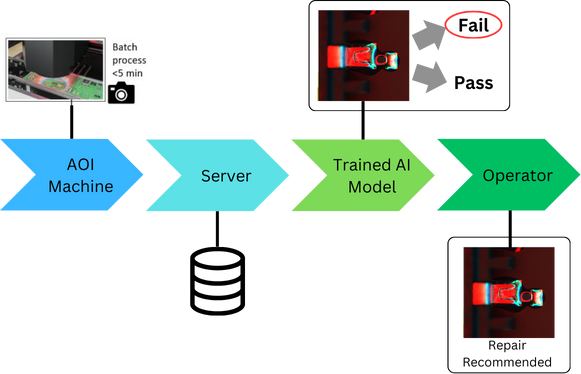
\includegraphics[width=1\linewidth]{Images/Solution_Pipeline.png}
    \caption{Solution Pipeline}
    \label{fig:solution pipeline}
\end{figure}

\subsection{Current Solution at Siemens}
\label{subsec:current solution at siemens}

Before presenting the problem statement, first we give an overview of current supervised solution which is implemented in Siemens AG.

\subsection{Thesis Objective}

Write thesis objective here

\subsection{Thesis Outline}
This thesis comprises of three main chapters: Theoretical Background, Methodology, and Results \& Discussion.-   % Introduction 
\clearpage
\chapter{Theoretical Background}

\section{Related Works}

Image Classification has experienced tremendous development over the last few decades, propelled by the increase in computational capabilities, large amounts of available data, and the development of sophisticated algorithms. This section provides an overview of the major advancements in the field of Image Classification, especially for its applications in industrial environments, such as electronics manufacturing. We will also explore the increasing significance of anomaly detection, emphasizing the transition from conventional supervised learning approaches to modern unsupervised learning methods.

\subsection{Evolution of Image Classification Techniques}

Image Classification is a critical task in the field of \gls{cv}, with numerous applications ranging from medical diagnostics to autonomous driving. Early image classification algorithms mainly relied on manual feature extraction, which involves domain experts designing these features, which could be used to differentiate between classes of images. These features were subsequently inputted into traditional machine learning algorithms like \glspl{svm} or \gls{k-nn} for classification \cite{LeCun2015}. Nevertheless, these techniques were limited by their dependence on handcrafted features, which could not effectively reflect intricate changes observed in real-world scenarios.

Subsequently, the introduction of \glspl{cnn} was a significant milestone in this field. They have introduced the concept of feature learning, whereby the network learns to extract relevant features from the raw image data by using numerous layers of convolutional filters \cite{NIPS2012_c399862d}. This groundbreaking study in \cite{NIPS2012_c399862d} on AlexNet architecture delivered exceptional results on the ImageNet dataset for image classification. This success triggered various research into network architectures that are deeper and more complex, such as VGGNet \cite{simonyan2015deepconvolutionalnetworkslargescale}, GoogLeNet \cite{7298594}, and ResNet \cite{he2016deep}.

Among these, the work on the introduction of ResNet by \cite{he2016deep} was highly significant as it addressed the issues of vanishing gradients that tormented earlier deep networks \cite{simonyan2015deepconvolutionalnetworkslargescale} \cite{7298594}. ResNet made it possible to train much deeper networks by incorporating residual connections, resulting in substantial improvement in accuracy over various image classification benchmarks. Thus, \glspl{cnn} were firmly established as the leading approach for tasks like image classification.

\subsection{Applications of Image Classification in Industrial Settings}

In the industrial sector, special attention is given to image classification applications in quality control processes, particularly in the context of automated visual inspection. Traditionally, the visual inspection process was carried out manually, where we had to rely on the experience of quality inspectors to ensure product quality. As a result of the varying levels of expertise among inspectors and the limitations of human abilities, this approach exhibits low efficiency, low accuracy, and inadequate real-time performance on a large-scale manufacturing process \cite{Gong_2020}.

With the rise of \gls{dl}, automated visual inspection systems are developed using \glspl{cnn} for defect detection in real-time. One of the most notable models in industrial applications is \gls{yolo} which is used for real-time object detection and has gained popularity in tasks requiring rapid image processing. The design of \gls{yolo} enables it to perform object detection in a single iteration over the network, rendering it highly efficient in cases where speed is critical. For example, during the PCB manufacturing process, \gls{yolo} can rapidly identify solder joints that do not meet quality standards. This offers a significant decrease in inspection times as compared to traditional manual techniques \cite{redmon2016you}.

Although \gls{cnn}-based models such as \gls{yolo} have demonstrated their effectiveness in most industrial applications, they do have certain limitations. One of the major obstacle is the requirement for a large labeled dataset to properly train such models. In many industrial applications, such as PCB inspection, defects are rare, and gathering labeled instances in large enough quantities for training purposes may become prohibitively expensive. In such instances, the labeling process is typically very labor- and knowledge-intensive, resulting in high costs and time consumption\cite{FINK2020103678}.

\subsection{Anomaly Detection in Electronics Manufacturing}

Due to the lack of labeled data, supervised learning methods are not feasible in certain scenarios. As a result, there has been a growing interest in exploring unsupervised learning methods for anomaly detection. Anomaly detection is the process of identifying patterns in data that deviate from expected behavior. This makes it an suitable solution in industrial applications for identifying defects where normal instances are well represented but anomalies are rare and diverse \cite{10.1145/1541880.1541882}.

In electronics manufacturing, anomaly detection plays an important role for tasks like solder joint inspection. Traditional techniques are based on models like probabilistic and distance-based. These techniques, are effective when dealing with simpler anomaly patterns but often faces difficulties when dealing with complex and high-dimensional data, as explained by \cite{PIMENTEL2014215}. This article points to the limitation of these methods because they reply on predefined thresholds and basic data assumptions, that fails to generalize on wide variety of anomalies.

Further expanding on this foundation, recent advancements in \gls{dl} introduced more sophisticated methods, particularly by employing autoencoders\cite{bank2021autoencoders}. Neural networks, namely \glspl{vae}\cite{Kingma_2019}, provides substantial improvements in presenting complex data distributions. These autoencoders learns compression and reconstruction of inputs through training on normal operational data, thereby building a model of 'normality' that allows it to find those anomalous instances with higher reconstruction errors indicating a deviation from the normal\cite{bank2021autoencoders}. This approach improves the detection of complex patterns of defects to help maintain the integrity of products produced in the manufacturing processes. Other variants of autoencoders, such \gls{vae}, deep autoencoders, has been investigated for anomaly detection and has shown promising results \cite{Kingma_2019}.

Another increasingly popular method is the \glspl{gan}\cite{goodfellow2014generativeadversarialnetworks} for anomaly detection. \glspl{gan} is consisting of two networks, namely a generator and a discriminator, both are trained simultaneously. The generator tries to produce data that is indistinguishable from the real one, while a discriminator strives to differentiate between real and generated data. In the context of anomaly detection, the generator is trained to generate normal instances, while the discriminator learns to identify any deviations from this normal distribution as anomalies \cite{schlegl2017unsupervisedanomalydetectiongenerative}.

%\subsubsection{Gaps in Current Research}

%Although significant advancements have been made in image classification and anomaly detectionusing both supervised and unsupervised learning methods, there are still certain gaps in the current research. The most obvious obstacle is the effective integration of the two approaches that maximizes the advantages of each other. Although supervised models, such as \gls{yolo}\cite{redmon2016you}, succeed well with abundant labeled data, they struggle in applications where labels are limited or where anomalies have not been well-defined. While unsupervised models entail more flexibility and typically require less labeled data, many are incapable of pulling off the same level of precision achieved with supervision when it comes to fine-grained classification tasks \cite{9347460}.




%In recent years, the exponential growth in deep learning research has revolutionized the field of Computer Vision. Much of this change has been led by Convolutional Neural Networks (CNNs), making highly accurate image recognition tasks possible[1]. Since then, ResNet and EfficientNet have further moved this needle by resolving issues like vanishing gradients and model scaling optimization[2][3]. Moreover, Vision Transformers (ViTs) have provided a new perspective in image classification by using transformer architectures primarily tailored for natural language processing[4]. These innovations have extended the scope of various areas in which deep learning applications can be applied in different industries, enhancing the ability to analyze and interpret complex visual data.

%The application of image classification techniques in the electronics manufacturing industry has shown significant promise. Automated visual inspection systems utilizing CNNs can effectively identify and classify defects in various manufacturing processes, reducing the reliance on manual inspection and minimizing human error. For example, deep learning models have been successfully applied to detect defects in automotive parts, textile production, and food processing, demonstrating their versatility and effectiveness [5]. Moreover, the integration of these techniques has streamlined quality control processes, enabling faster and more accurate identification of defects, which is crucial for maintaining high standards of product quality and efficiency in production lines [6].

%Advances in anomaly detection, particularly through unsupervised learning, have also played a critical role in the manufacturing sector. Traditional methods often rely on labeled datasets, which can be time-consuming and costly to generate. Unsupervised anomaly detection techniques, such as autoencoders, variational autoencoders (VAEs), and generative adversarial networks (GANs), have alleviated this dependency by identifying deviations from normal patterns without the need for extensive labeling [7]. These methods have been applied to detect anomalies in a wide range of manufacturing contexts, from monitoring machinery health to ensuring the integrity of assembled products. By leveraging the inherent patterns in the data, unsupervised learning approaches have enabled more scalable and adaptable solutions for anomaly detection [8][9].

%The continuous evolution of these technologies underscores the transformative impact of deep learning on the manufacturing industry. By integrating advanced image classification and anomaly detection techniques, manufacturers can achieve more efficient and accurate inspection processes, ultimately leading to improved product quality and operational efficiency. This ongoing research and development highlight the potential for even greater advancements in the future, as deep learning models become more sophisticated and capable of addressing increasingly complex manufacturing challenges [10].

%References

%[1] Krizhevsky, Alex, Ilya Sutskever, and Geoffrey E. Hinton. "Imagenet classification with deep convolutional neural networks." Advances in neural information processing systems 25 (2012).
%[2] He, Kaiming, et al. "Deep residual learning for image recognition." Proceedings of the IEEE conference on computer vision and pattern recognition. 2016.
%[3] Tan, Mingxing, and Quoc V. Le. "EfficientNet: Rethinking model scaling for convolutional neural networks." International Conference on Machine Learning. PMLR, 2019.
%[4] Dosovitskiy, Alexey, et al. "An image is worth 16x16 words: Transformers for image recognition at scale." arXiv preprint arXiv:2010.11929 (2020).
%[5] Bhandarkar, Suchendra M., et al. "Deep learning based quality inspection in manufacturing." Procedia Manufacturing 26 (2018): 998-1006.
%[6] Zhang, Xiaolei, et al. "Deep learning-based quality inspection for manufacturing." IEEE Access 7 (2019): 61232-61245.
%[7] An, Jinwon, and Sungzoon Cho. "Variational autoencoder based anomaly detection using reconstruction probability." Special Lecture on IE 2.1 (2015).
%[8] Ruff, Lukas, et al. "Deep One-Class Classification." International Conference on Machine Learning. PMLR, 2018.
%[9] Kiran, B Ravi, Dilip Thomas, and Ranjith Parakkal. "An overview of deep learning based methods for unsupervised and semi-supervised anomaly detection in videos." Journal of Imaging 4.2 (2018): 36.
%[10] Bergmann, Paul, et al. "Uninformed students: Student-teacher anomaly detection with discriminative latent embeddings." Proceedings of the IEEE/CVF Conference on Computer Vision and Pattern Recognition. 2020.

%\subsection{Machine Learning}

%Machine Learning is a subdomain of Artificial Intelligence that encompasses various techniques able to automatically discover patterns in data and use those patterns to predict future data[1].

\section{Supervised Image Processing}
\label{sec:supervised}

Supervised image processing is a subset of \gls{ml} where a model is trained using labeled dataset. Labeled dataset means that each image in that dataset is tagged with its correct output label or category. With this approach, the model can learn to map inputs to specific outputs \cite{geeksforgeeks-sup-unsup}.

\subsection{Artificial Neural Networks (ANNs)}

\gls{ann} are computational processing systems that are inspired by how biological nervous systems such as the human brain functions. \gls{ann} mainly consists of numerous interconnected computational nodes, known as neurons, which are intertwined in a distributed manner to collectively learn from te input and optimize the final output \cite{oshea2015introductionconvolutionalneuralnetworks}.

\begin{figure}[ht!]
    \centering
    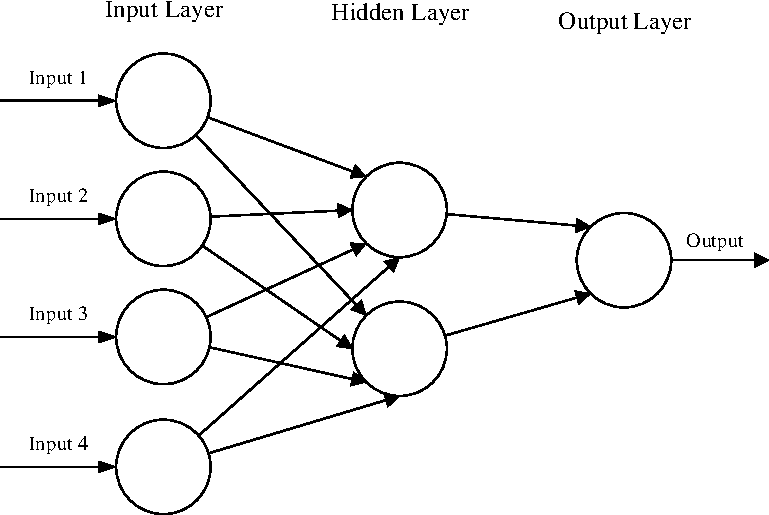
\includegraphics[width=1\linewidth]{Images/ann_architecture.pdf}
    \caption{\gls{ann} is a three-layer \gls{fnn} consisting of an input layer, a hidden layer, and an output layer \cite{oshea2015introductionconvolutionalneuralnetworks}.}
    \label{fig:ann architecture}
\end{figure}

The figure \ref{fig:ann architecture} shows the basic structure of a \gls{ann}. Input data will be loaded in the form of multidimensional vector into the input layer, then it will be distributed into the hidden layer. Then hidden layers will make decisions based on previous layer and evaluate how a stochastic change improves the final output, this process is know as learning. When multiple hidden layers are stacked next each other it is known as \gls{dl} \cite{oshea2015introductionconvolutionalneuralnetworks}.

\subsection{Convolutional Neural Networks (CNNs)}

\glspl{cnn}\cite{726791} is an extended version of \gls{ann} which is primarily used for feature extraction from a grid-like matrix dataset \cite{GeeksforGeeks2024}. \glspl{cnn} is similar to traditional \gls{ann} in terms of that they consists of neurons that self-optimize through learning. Each neuron will receive input and perform operations like scalar product followed by a non-linear function, which is the basis of many \gls{ann}. The only significant difference between \glspl{cnn} and traditional \gls{ann} is that \glspl{cnn} are mainly used on images in the field of pattern recognition. This enables the encoding of image-specific features into the architecture, making it more suitable for image-focused tasks while also reducing the parameters required for model configuration \cite{oshea2015introductionconvolutionalneuralnetworks}.

The term \glspl{cnn} indicates that the network uses a mathematical operation called \textbf{convolution}. \glspl{cnn} are neural networks that in the place of general matrix multiplication uses convolution in at least one of the layers \cite{Goodfellow-et-al-2016}.

\subsubsection*{\gls{cnn} Architecture :}

Basic \gls{cnn} architecture consists of three types of layers, they are \textbf{convolutional layers}, \textbf{pooling layers}, and \textbf{fully connected layers}. When these layers are stacked together, then a \gls{cnn} architecture is formed. Figure \ref{fig:cnn architecture} shows \gls{cnn} architecture for MNIST\cite{6296535} classification.


\begin{figure}[ht!]
    \centering
    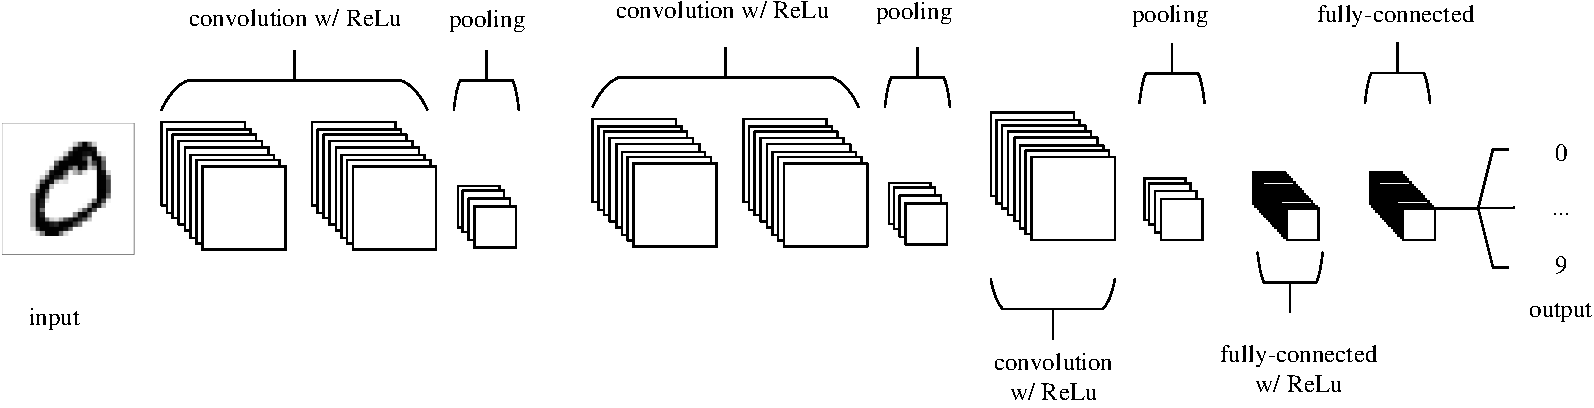
\includegraphics[width=1.1\linewidth]{Rohit_Master_Thesis//Images/cnn_architecture.pdf}
    \caption{A common \gls{cnn} architecture \cite{oshea2015introductionconvolutionalneuralnetworks}}
    \label{fig:cnn architecture}
\end{figure}

The functionality of \gls{cnn} architecture shown above can be broken down basically into four key areas.

1. Similar to other types of \gls{ann}, the input layer holds the images pixel values \cite{oshea2015introductionconvolutionalneuralnetworks}.

2. Convolutional layer will determine the output of neurons that are linked to local regions of input by calculating the scalar product of their weights and the corresponding input volume region. The \gls{relu} aims to apply an 'elementwise' activation function like sigmoid to the output generated by the preceding's layer's activation \cite{oshea2015introductionconvolutionalneuralnetworks}.

3. The pooling layer will perform downsampling along the spatial dimensions of the input, this further reduces the number of parameters in the activation \cite{oshea2015introductionconvolutionalneuralnetworks}.

4. The fully connected layers will then perform the same functions as that in a standard \gls{ann}, aiming to produce class scores from the activations, for classification purposes. To improve performance, it's also recommended to use \gls{relu} between these layers \cite{oshea2015introductionconvolutionalneuralnetworks}. 

By using this simple transformation technique, \glspl{cnn} can transform the original input layer by layer, by using convolutional and downsampling techniques producing class scores for classification and regression purposes \cite{oshea2015introductionconvolutionalneuralnetworks}. Lets look at the main components of the \gls{cnn} architecture in detail.

\subsubsection*{Convolutional Layer :}

Convolutional layer plays important role in the \glspl{cnn} functionality. The layers parameters concentrate on the use of learnable \textbf{kernels}. These kernels are the set of learnable parameters.

These kernels are usually small in spatial dimensions, however spreads entirely along the depth of the input. Upon the data entering a convolutional layer, it convolves each filter across the spatial dimensions of the input to generate a 2D activation map as shown in figure \ref{fig:convolutional layer} \cite{oshea2015introductionconvolutionalneuralnetworks}.

%\begin{figure}
%    \centering
%    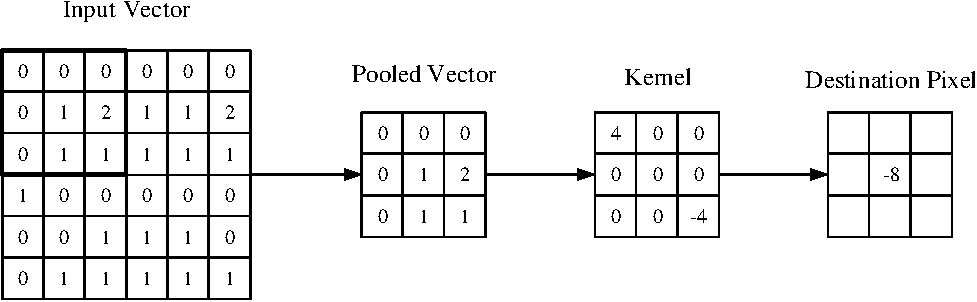
\includegraphics[width=1.1\linewidth]{Rohit_Master_Thesis//Images/conv_layer.pdf}
%    \caption{A visual representation of a covolutional layer. The centre element of the kernel is positioned over the input vector, from which then a weighted sum of itself and any nearby pixels is calculated and replaced \cite{oshea2015introductionconvolutionalneuralnetworks}.}
%    \label{fig:convolutional layer}
%\end{figure}

\begin{figure}[ht!]
    \centering
    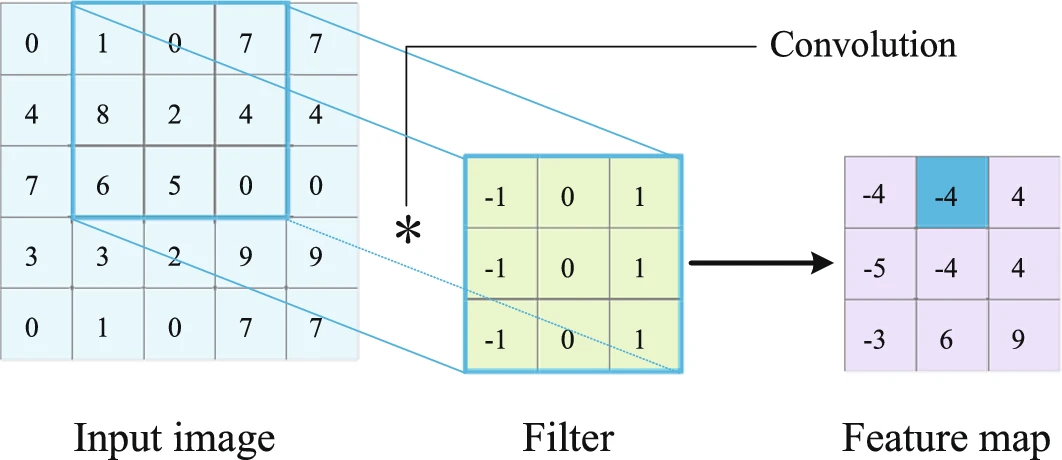
\includegraphics[width=1\linewidth]{Rohit_Master_Thesis//Images/conv_layer_v2.png}
    \caption{The convolution operation involves the sliding of a convolution kernel(filter) over the input vector, where the kernel is multiplied by the pixel value at the corresponding positions of the input, and summing them to produce a feature map \cite{Zhao2024}.}
    \label{fig:convolutional layer}
\end{figure}

As the kernel glides through the input, it calculates the scalar product for each value in that kernel. Through this the network will learn kernels that activates upon they detect a specific feature at a given spatial position of the input. These are commonly referred to as activations. Each kernel will have a corresponding activation map, which will be stacked along the depth dimension to form complete output volume from the convolutional layer \cite{oshea2015introductionconvolutionalneuralnetworks}.

To mitigate the problem of \gls{ann} where the models gets too big to train effectively due to the full-connected nature of standard \gls{ann} neurons, each neuron in a convolutional layer is connected only to a small region of the input, known as \textbf{receptive field}. The connectivity depth is almost always equal to the input depth \cite{oshea2015introductionconvolutionalneuralnetworks}. To understand this, lets consider an example, if the network receives an input image measuring $64\times64\times3$(representing an RGB image), with the receptive field being of the size $6\times6$, each neuron will have a total of 108 weights with in the convolutional layer($6\times6\times3$, with 3 representing the amount of connectivity across the depth of the volume). Whereas a standard neuron in other forms of \gls{ann} would have $12,288$ weights each \cite{oshea2015introductionconvolutionalneuralnetworks}.

By optimizing its output convolutional layers can also significantly reduce the complexity of the model. These are optimized by three hyperparameters: depth, stride, and setting zero-padding.

The \textbf{depth} of the output volume can be set manually using the number of neurons within the convolutional layer corresponding to the same region in the input. Although reducing this hyperparameter can significantly reduce the total number of neurons of the network, it can also significantly reduce the model's pattern recognition capabilities \cite{oshea2015introductionconvolutionalneuralnetworks}.


\textbf{Stride} is the number of rows and columns that the receptive field will move across the input's spatial dimension \cite{Zhao2024}. For example, with stride set to 1, then the significantly overlapping receptive field will produce very large activations, while a larger value of stride will reduce overlapping and produce an output of lower spatial dimensions \cite{oshea2015introductionconvolutionalneuralnetworks}.

\textbf{Zero-Padding} is a simple process of padding the border of the input with zeros, it's an effective way to enhance control of the dimentionality of the output volumes \cite{oshea2015introductionconvolutionalneuralnetworks}.

We can calculate the spatial dimensionality of convolutional layers output by using the following formula: 

\[
    \frac{(V - R) + 2Z}{S + 1}
\]

Here the V denotes the input volume size(height$\times$width$\times$depth), R denotes the receptive field size, Z denotes the zero-padding set, and S denotes the stride. If the result from the above formula is not a whole integer then the stride has been set incorrectly, and the neurons wont be able to fit across the given input \cite{oshea2015introductionconvolutionalneuralnetworks}.

Despite these optimizations, models can still be huge while using high dimensionality input like images. To further reduce the number of parameters significantly within the convolutional layer \textbf{parameter sharing} is used. It works on the assumption that if a feature from one spatial region is useful for computation, then its likely to be useful in another region as well \cite{oshea2015introductionconvolutionalneuralnetworks}.

\subsubsection*{Pooling layer :}

The pooling layers reduces the dimensionality of the feature representation, thus reducing the number of parameters and computational complexity of the model. Pooling layer operates on each activation map in the input, and reduces its dimensionality using the 'Max' function. Max-pooling layers is one of the most common types of pooling used in \glspl{cnn}. It selects the maximum activity value of all neurons for the representation for the particular region and extract the most essential feature from the input feature map \cite{Zhao2024}. A $2\times2$ kernels is applied with a stride of 2 across the spatial dimensions of the input reduces the activation map by $75\%$ of the original size, while preserving the depth volume of the feature map \cite{oshea2015introductionconvolutionalneuralnetworks}. 

Average pooling computes the arithmetic mean of all the elements within the region, resulting in the mean value of the local response from the extracted feature mapping \cite{Zhao2024}. The figure \ref{fig:max pooling} shows max pooling operation where the maximum value is used, and figure \ref{fig:average pooling} shows the average pooling operation, which performs the average operation to get the value.

\begin{figure}[H]
    \centering
    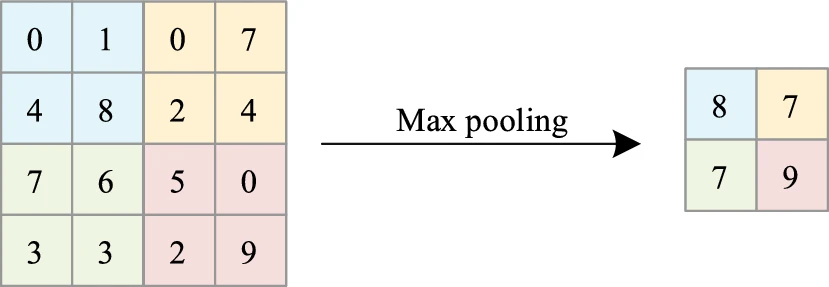
\includegraphics[width=1\linewidth]{Rohit_Master_Thesis//Images/max_pooling.png}
    \caption{Max pooling \cite{Zhao2024}}
    \label{fig:max pooling}
\end{figure}

\begin{figure}[H]
    \centering
    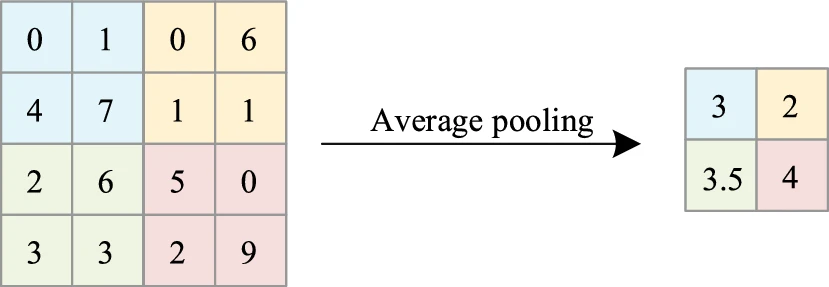
\includegraphics[width=1\linewidth]{Rohit_Master_Thesis//Images/average_pooling.png}
    \caption{Average pooling \cite{Zhao2024}}
    \label{fig:average pooling}
\end{figure}

\subsubsection*{Fully-Connected Layer :}

The fully-connected layer contains neurons which are directly connected to the neurons in the two neighboring layers, with no connections to any neurons within itself. It is similar to the way neurons are arranged in traditional \gls{ann} as can be seen in the figure \ref{fig:ann architecture} \cite{oshea2015introductionconvolutionalneuralnetworks}.

\subsubsection*{Activation Function :}

Activation functions plays a crucial role in neural networks, strengthening the network's representational and learning capabilities, by learning the abstract features through nonlinear transformation \cite{dubey2022activationfunctionsdeeplearning}. With the introduction of the activation functions, the neural network can approximate any nonlinear function, making it applicable to a wide range of nonlinear models \cite{Zhao2024}. Some of the activation functions common properties are:

1. It should add the nonlinear curvature in the optimization landscape to enhance training convergence of the network;

2. It shouldn't significantly increase the computational complexity of the model;

3. During training it shouldn't hamper the gradient flow;

4. It should preserve the data distribution and facilitate better network training \cite{dubey2022activationfunctionsdeeplearning}.

Here we will look at the most common and widely used activation functions, including Sigmoid, Tanh, Softmax, \gls{relu}, and Leaky \gls{relu}.

\textbf{1. Sigmoid Activation Function :}

The Sigmoid function, or the logistic function, ranges from 0 to 1. As can be seen from the figure \ref{fig:sigmoid tanh function curve}, sigmoid can be used to normalize the output, as well as probability-based predictions \cite{Zhao2024}. The following is the sigmoid functions mathematical formula :

\[ 
    f(x) = \frac{1}{1 + e^{-x}}
\]

Figure \ref{fig:sigmoid tanh function curve} shows that the sigmoid gradient is smooth, preventing output values from jumping. Nevertheless, there are many problems with using Sigmoid, like when the activation is near 0 or 1 the chances of vanishing gradient are high. There is also slow gradient descent's convergence due to non-zero-centered output. Finally, due to sigmoid functions exponential operation, the computation time of the model increases as well \cite{Zhao2024}.


\begin{figure}[!ht]
    \centering
    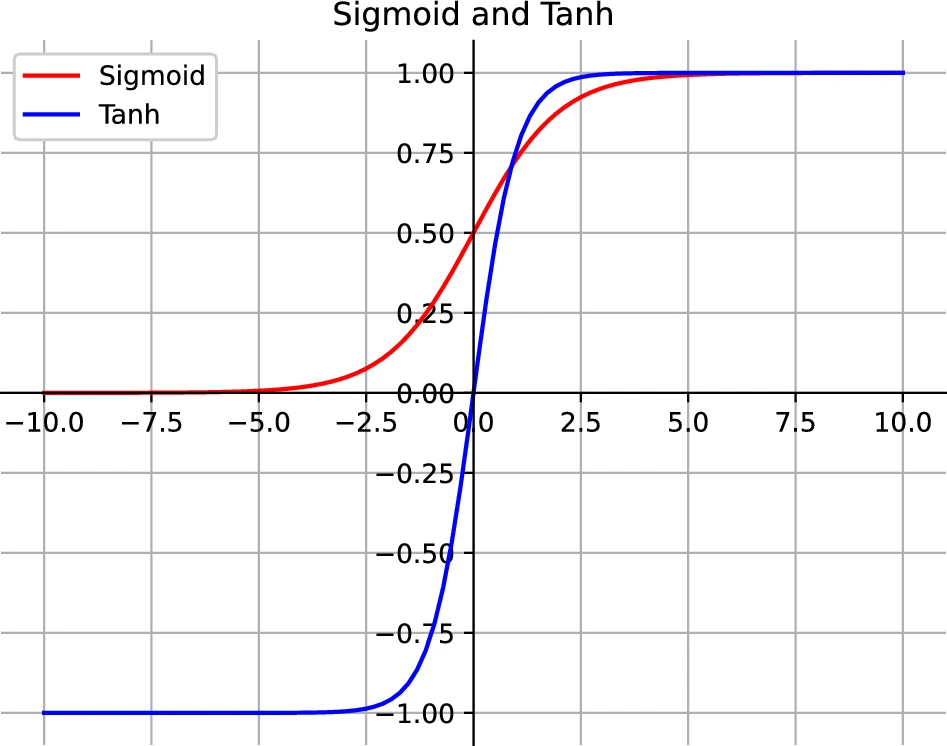
\includegraphics[width=1\linewidth]{Rohit_Master_Thesis//Images/sigmoid_tanh_af.png}
    \caption{Sigmoid and Tanh activation function curve \cite{Zhao2024}}
    \label{fig:sigmoid tanh function curve}
\end{figure}

\textbf{2. Tanh Activation Function :}

The hyperbolic tangent activation function(HTAF), or tanh, compresses the input vector in the range of -1 to 1, and also offers a zero-centered output. The below formula and the figure \ref{fig:sigmoid tanh function curve} shows the tanh curve and mathematical representation:

\[
    f(x) = \frac{2}{1 + e^{-2x}} - 1
\]

From the figure \ref{fig:sigmoid tanh function curve} we can see that tanh and sigmoid function are relatively similar S-shaped curves. Tanh and Sigmoid have the following relationship:

\[
    Tanh(x) = 2Sigmoid(2x) - 1
\]

In practice tanh is used more than sigmoid as it solves sigmoid function not centering the output to zero problem. However, like sigmoid, tanh also suffers from vanishing gradient problem for extreme input values \cite{Zhao2024}.

\textbf{3. Softmax Activation Function :}

Softmax activation function is used for multi-class classification problems. It compresses the input vectors into probabilities in the range of 0 to 1, all of which sum up to 1. In K classification task, the generated probabilities can be used to represent each category, with larger value indicating higher probability that it belongs to that particular category \cite{Zhao2024}. Figure \ref{fig:softmax function curve} shows the softmax function curve, and the below formula shows how softmax is formulated mathematically:

\[
    f(x) = \frac{e^{x_i}}{\sum_{j=1}^{k} e^{x_j}}
\]

\begin{figure}[H]
    \centering
    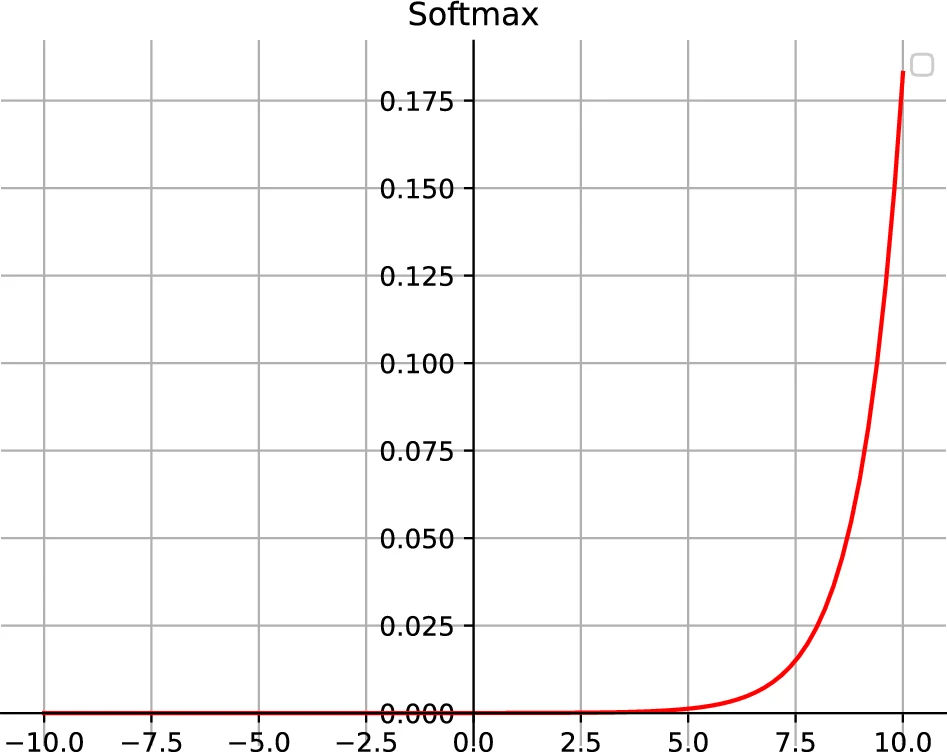
\includegraphics[width=1\textwidth]{Rohit_Master_Thesis//Images/softmax.png}
    \caption{Softmax activation function curve \cite{Zhao2024}}
    \label{fig:softmax function curve}
\end{figure}

When the softmax function encounters negative input value, the gradient becomes zero, therefore the weights for activation in that region will not update throughout backpropagation, resulting in a dead neuron that never activated \cite{Zhao2024}.

\textbf{4. ReLU Activation Function :}

ReLU, or Rectified Linear Unit is a segmented linear function, as shown in the figure \ref{fig:relu function curve}. It is a fast, simple activation function which is essentially a ramp function given by the following formula:

\[
    f(x) = max(0,x)
\]


\begin{figure}[H]
    \centering
    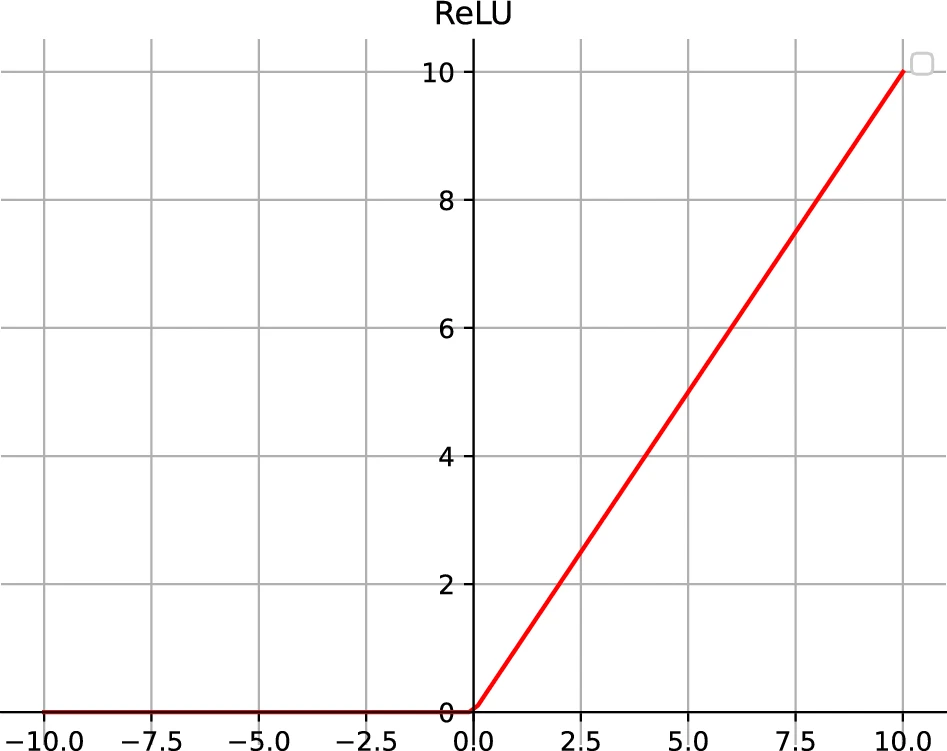
\includegraphics[width=1\linewidth]{Rohit_Master_Thesis//Images/relu_af.png}
    \caption{ReLU function curve \cite{Zhao2024}}
    \label{fig:relu function curve}
\end{figure}

When the input is positive, the derivative is 1, which improves the vanishing gradient problem and also speeds up the gradient descent convergence. Its also faster than sigmoid and tanh functions, due to ReLU function only has linear relationships. But this function suffers from dying ReLU problem, which is when the input is negative, the gradient will be exactly zero and the neurons will most likely die during training \cite{Zhao2024}.

\textbf{5. Leaky ReLU Activation Function :}

Leaky ReLU addresses the dying ReLU problem to some extent by introducing very small linear components for negative inputs to solve zero gradients assostiated with negatives, and extending the range of ReLU. Although Leaky ReLU has all the features of ReLU, in practice its not always the case that Leaky ReLU is better than ReLU \cite{Zhao2024}. Below is the mathematical formulation of Leaky ReLU and figure \ref{fig:leaky relu function curve} shows its function curve.

\[
f(x) =
\begin{cases} 
    x, & \text{if } x \geq 0 \\
    ax, & \text{if } x < 0 
\end{cases}
\]

\begin{figure}[H]
    \centering
    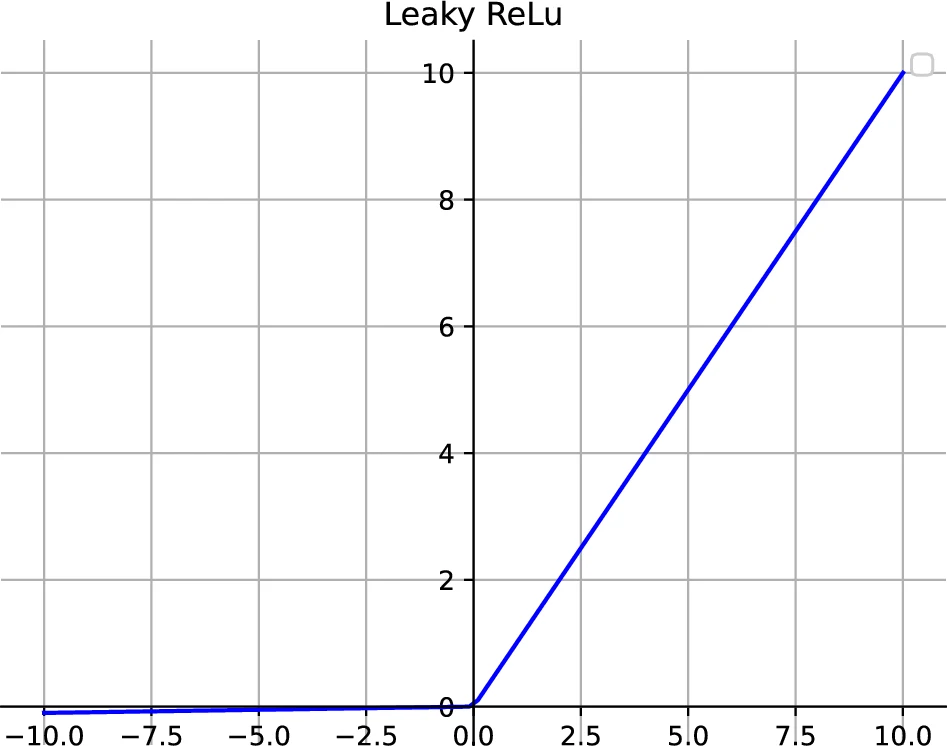
\includegraphics[width=1\linewidth]{Rohit_Master_Thesis//Images/leaky_relu_af.png}
    \caption{Leaky ReLU function curve \cite{Zhao2024}}
    \label{fig:leaky relu function curve}
\end{figure}

\subsection{ResNet}
\label{subsec:ResNet}

Deep Convolutional neural networks has led to numerous advancements in image classification. The depth of the network plays a crucial role in this achievement, but deeper networks still faces a critical problem of \textbf{degradation}. The degradation problem occurs when deeper neural networks starts to converge: with increasing network depth the accuracy gets saturated and then rapidly declines. This is caused by increase in number of layers which results in higher training error. To address this degradation problem a deep residual learning framework was proposed. In this framework, instead of relying on each stacked layer to directly match a specific underlying mapping, the layers are designed to fit a residual mapping \cite{he2016deep}.

\begin{figure}[ht!]
    \centering
    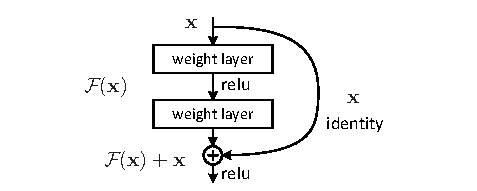
\includegraphics[width=1.2\linewidth]{Rohit_Master_Thesis//Images/residual_block.pdf}
    \caption{A residual block \cite{he2016deep}}
    \label{fig:residual block}
\end{figure}

\subsubsection*{Residual Learning :}

As mentioned above instead of expecting stacked layers to approximate mapping function H(x), where x denotes the inputs to the first of these stacked layer. The layers are explicitly let to approximate a residual function $F(x) := H(x) - x$. The original function then becomes $F(x) + x$. This makes the learning process much easier, although it's expected that both forms can asymptotically approximate the desired functions \cite{he2016deep}.

The above mentioned residual learning is applied to every few stacked layers. The structure of a residual block is shown in the figure \ref{fig:residual block}. The basic building block can be defined for this approach as:

$ y = F(x, \left\{ W_{i}\right\}) + x$.

Here x, and y represents the input and output vectors of the considered layers, The function $F(x, \left\{ W_{i}\right\})$  represents the residual mapping to be learned. The operation $F + x$ is performed by a \textbf{shortcut connection} also known as skip connection, and element-wise addition as shown in figure \ref{fig:residual block}. This shortcut connections doesn't introduce any extra parameters or computational complexity, except for the minor element-wise addition. This ensures a fair comparison between plain and residual networks  which have the same number of parameters, width, depth, and computational cost \cite{he2016deep}.

\subsubsection*{Network Architecture :}

\begin{figure}[H]
    \centering
    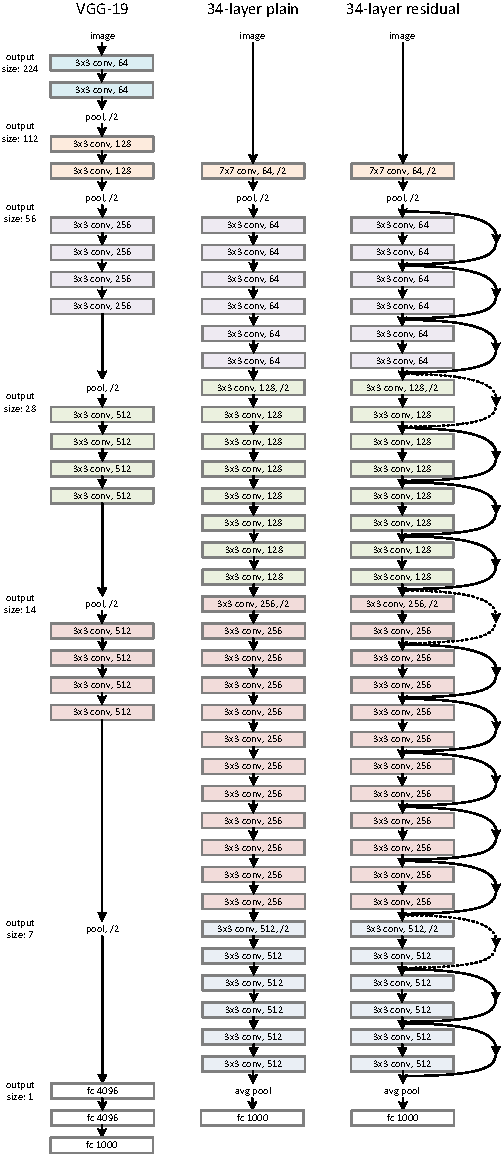
\includegraphics[width=0.6\textwidth]{Rohit_Master_Thesis//Images/resnet_arch.pdf}
    \caption{Network architecture example: Left: VGG-19 model serves as a reference. Middle: a plain network consisting of 34 parameter layers. Right: a residual network with 34 parameter layers \cite{he2016deep}.}
    \label{fig:resnet architecture}
\end{figure}

As can be seen in the figure \ref{fig:resnet architecture} two models are described. The plain baseline network(figure \ref{fig:resnet architecture}, middle) draws inspiration from the philosophy of VGG nets\cite{simonyan2015deepconvolutionalnetworkslargescale} (Figure \ref{fig:resnet architecture}, left), which mostly uses $3\times3$ filters. It maintains the time complexity per layer by doubling the number of filters when feature map size is halved. Downsampling is performed by convolutional layer with stride 2, the network ends with global average pooling layer followed by a 1000-way fully connected layer with softmax \cite{he2016deep}.

Based on the plain network, short connections are added which transforms the network into its counterpart residual version. Identity shortcuts are used for matching input-output dimensions(solid line shortcuts in figure \ref{fig:resnet architecture}). For when dimensions increases(dotted line shortcuts in figure \ref{fig:resnet architecture}), either the shortcut performs identity mapping, with zero-padding, or projection shortcuts($1\times1$ convolutions) are used \cite{he2016deep}.

\subsubsection*{Performance :}

The 18-layer and 34-layer \gls{resnet} shows that the deeper 34-layer \gls{resnet} performs better than the 18-layer \gls{resnet} by 2.8\%. Also the 34-layer \gls{resnet} demonstrates a considerable reduction in training error and shows good generalization to the validation data. This shows that the degradation problem is well tackled in this setting leading to accuracy gains from increased depth. Compared to the plain network(figure \ref{fig:resnet architecture}, middle), the 34-layer \gls{resnet} reduced the top-1 error by $3.5\%$, this verifies the efficacy of residual learning on very deep networks. It was also observed that 18-layer plain networks are more accurate, but the 18-layer \gls{resnet} converges faster \cite{he2016deep}.

\subsubsection*{Deeper Bottleneck Architectures :}

To scale the networks to 50, 101, and 152 layers, a bottleneck design is used, where the building blocks are modified as bottleneck layers, in which the residual function is stacked with 3 layers($1\times1$, $3\times3$, $1\times1$ convolutions). The $1\times1$ are responsible for dimensions reduction filled by restoration, which creates a bottleneck in the $3\times3$ layer with smaller input and output dimensions \cite{he2016deep}.

\textbf{50-layer \gls{resnet}:} In this architecture each 2-layer block in a 34-layer network is replaced with a 3-layered bottleneck block, which results in a 50-layer \gls{resnet} \cite{he2016deep}.

\textbf{101-layer \& 152-layer \glspl{resnet}:} 3-layer blocks are used for the construction of 101-layer and 152-layer \glspl{resnet}. Even when the depth is increased a lot the 152-layer \gls{resnet} still has lower complexity than VGG-16/19 networks \cite{he2016deep}.

The 50/101/152-layer \glspl{resnet} show significantly higher accuracy compared to the 34-layer versions. No degradation problem is observed, due to which high accuracy can be achieved \cite{he2016deep}.

\subsection{Vision Transformer}

Transformers introduced by \cite{vaswani2017attention} has become the go to model in \gls{nlp} related tasks. Transformer's computational efficiency and scalability allows for exceptional model training with over 100B parameters. However, when it comes to \gls{cv}, convolutional architectures like ResNet\cite{he2016deep} are still dominant. Therefore inspired by the success of transformers in \gls{nlp}, standard transformer was directly applied to images, with minimal modifications. For this images were split into patches, then the transformer was given the linear embeddings of these patches as input. These images patches are treated the same way as token(words) as in \gls{nlp} tasks, and the training is carried in supervised fashion \cite{dosovitskiy2020image}.

\subsubsection*{Architecture :}

An overview of the architecture of the model is shown in the figure \ref{fig:vit architecture}. The standard transformer takes 1D sequence of token embeddings as input.To process 2D images, firstly the image is reshaped into flattened 2D patches, these is called the patch embeddings \cite{dosovitskiy2020image}. 

\begin{figure}[ht!]
    \centering
    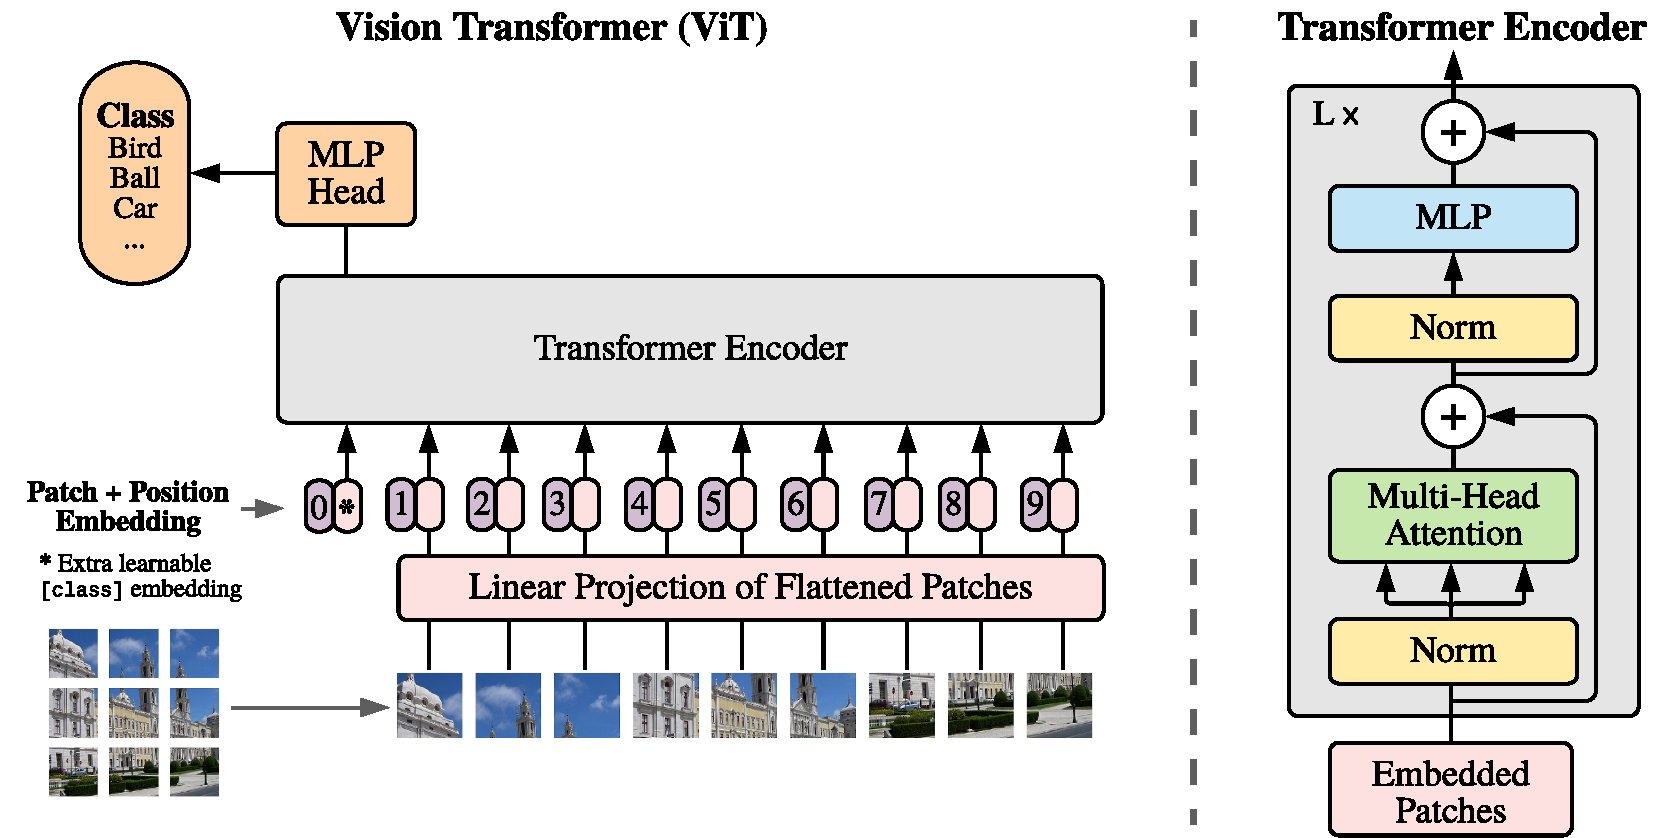
\includegraphics[width=1\linewidth]{Rohit_Master_Thesis//Images/vit_architecture.pdf}
    \caption{This is the proposed \gls{vit} architecture. Here an image is split into patches of fixed size, each of them is then linearly embedded, with that positional embedding is added, and then the resulting sequence is given as input to a standard transformer encoder. To perform classification, a "classification token" is added to the sequence \cite{dosovitskiy2020image}.}
    \label{fig:vit architecture}
\end{figure}

Similar to BERT's [class] token, a learnable classification token is prepended to the sequence of the patch embeddings. Its output from the transformer encoder is used as image representation for classification. During both training and fine-tuning, a classification head is attached to this output, which consists of a \gls{mlp} with one hidden layer during pre-training and a single linear layer at fine-tuning time. Positional embeddings are also added to the patch embeddings for retaining the positional information. The transformer encoder, as seen at the right side of the figure \ref{fig:vit architecture}, has alternating layers of \gls{msa} and \gls{mlp} blocks. Each block also includes \gls{ln}, and residual connections, these are applied before each block and after each block respectively. The \gls{mlp} consists of two layers with a GELU activation function. These layers processes the sequence of patch embeddings and the [class] token \cite{dosovitskiy2020image}.

\subsection{Data-efficient image Transformers (DeiT)}

\gls{deit} was introduced in the paper \cite{pmlr-v139-touvron21a}, which unlike \gls{vit}\cite{dosovitskiy2020image} doesn't need large-scale training, and uses only Imagenet as training set, and also need fewer computational resources. \gls{deit} introduced a token-based distillation strategy to distill information into the model \cite{pmlr-v139-touvron21a}.

\subsubsection*{Distillation strategy :}

For a teacher model a strong image classifier is used, it can be either a \gls{cnn} or a mixture of classifiers. One of the key innovation in \gls{deit} is the introduction of "distillation token". This procedure is shown in the figure \ref{fig:deit distillation token}, this distillation token is used similar to the class token which is added to the initial embeddings. It interacts with other tokens using the self-attention. The distillation token embedding is output by the network after the last layer, and it is optimized by using the distillation component of the loss. This distillation embedding helps the model to learn from the output of the teacher, which remains complimentary to the class embedding \cite{pmlr-v139-touvron21a}.

\begin{figure}[ht!]
    \centering
    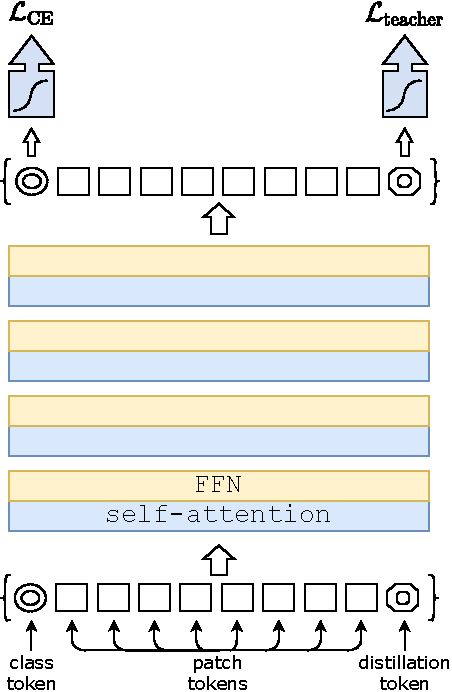
\includegraphics[width=0.5\linewidth]{Rohit_Master_Thesis//Images/deit_distillation_token.pdf}
    \caption{\gls{deit} distillation procedure\cite{pmlr-v139-touvron21a}.}
    \label{fig:deit distillation token}
\end{figure}

\subsection{Class-Attention in Image Transformers (CaiT)}

\gls{cait} is vision transformer type, it makes two main modifications to the original \gls{vit} architecture. Firstly, a new layer scaling method termed as LayerScale is used, which adds a learnable diagonal matrix at the output of each residual block. This matrix is initialized close to 0, which improves the training dynamics. Secondly, class-attention layers are also introduced. This creates an architecture in which the transformer layers which involves self-attentiom between the patches are separated from the class-attention layers, which are devoted to extract the content of the processed patches into a single vector, so it can be linear classifiers input \cite{touvron2021going}. 

\subsubsection*{Architecture :}

The \gls{cait} consists of two processing stages as can be seen in the figure \ref{fig:cait architecture}.

\paragraph{Self-Attention Stage :} In this stage, the CLS class token is inserted later in the transformer. This resolves the inconsistency of the first layers of the transformer, which are then entirely used for performing self-attention between patches only \cite{touvron2021going}. 

\begin{figure}
    \centering
    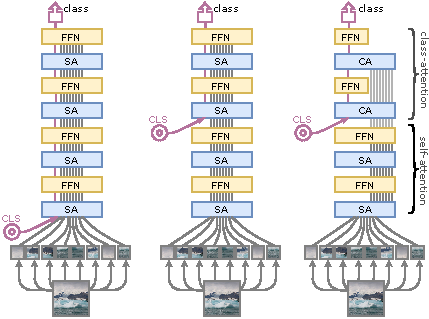
\includegraphics[width=0.75\linewidth]{Rohit_Master_Thesis//Images/cait_architecture.pdf}
    \caption{In this figure, the original \gls{vit} is on the left, here the CLS token is inserted with patch embeddings. This is counterproductive, as the same weights are used for two different purposes. In the middle architecture, the author shows that inserting the CLS token later on improves performance. And further in the \gls{cait} architecture(right), the patch embeddings are frozen when inserting CLS tocken to save computational resources. So the last part of the network, usually the last 2 layers are fully focused on summarizing the information to will be given as an input to the linear classifier \cite{touvron2021going}.}
    \label{fig:cait architecture}
\end{figure}

\paragraph{Class-Attention Stage :} It is a set of layers which compiles the patch embeddings into a class embedding CLS that is then given to a linear classifier. Here only the class embeddings are updated. But the main difference is that, within \gls{cait} architecture, the information is not copied from class embedding to the patch embeddings during the forward pass.

\subsection{You Only Look Once (YOLO)}
\label{subsec:yolo}

The human visual system operates with amazing speed and accuracy, which helps us perform complex tasks like driving with minimal conscious thought. Similarly, fast and accurate algorithms for object detection could facilitate computers to drive a car without the need of specialized sensors, assistive devices to provide real-time scene information to human users, this could pave the way the way for better responsive robotic systems. The object detection algorithms before \gls{yolo} used classifiers and repurposed them to detect objects by evaluating it across different locations and scale it in a test image. These methods are quite slow and complex to optimize \cite{redmon2016you}.

\gls{yolo} approaches the object detection by treating it as a single regression problem, directly mapping image pixels to bounding box coordinates and class probabilities. That means, you only look once \gls{yolo} at an image to predict and present what the object is and what its location. As shown in the figure \ref{fig:yolo system}, a single \gls{cnn} can predict multiple bounding boxes and at the same time their class probabilities. It's trained on full images and focuses on optimizing detection performance directly \cite{redmon2016you}.

\begin{figure}[H]
    \centering
    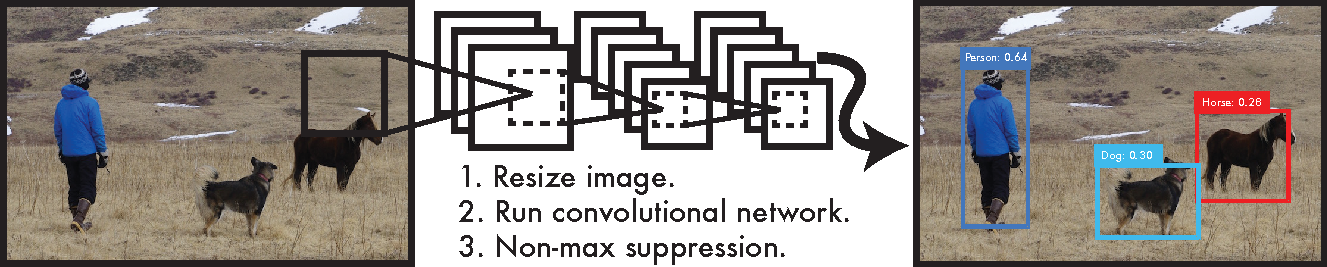
\includegraphics[width=1\linewidth]{Rohit_Master_Thesis//Images/yolo_system.pdf}
    \caption{\gls{yolo} Detection System: \gls{yolo} makes the image processing very simple. It first resizes the image, followed by running a single \gls{cnn} on image, and then finally giving thresholding value to the detections based on model's confidence \cite{redmon2016you}.}
    \label{fig:yolo system}
\end{figure}


\subsubsection*{ How \gls{yolo} works :}

As stated before \gls{yolo} unifies the separate components of object detection into a single neural network. This network uses features from the complete image for the prediction of all bounding boxes across all classes at the same time. \gls{yolo} enables training from start to finish and achieves real-time speeds, all while ensuring a high level of average precision. \gls{yolo} divides the input image into an $S\times S$ grid. Each grid cell is responsible for detecting an object whose center falls into that grid cell. Every grid cell predicts bounding boxes and its confidence scores. This score reflects models confidence in the box containing an object, as well as how accurate the predicted box is. If object is detected then the confidence score should be equal to \gls{iou} between the ground truth and the predicted box, else if no object is detected then the confidence score should be zero. At the test time the conditional class probabilities and the box confidence predictions are multiplied to get the final detection as shown in the figure \ref{fig:yolo model} \cite{redmon2016you}.

\begin{figure}[H]
    \centering
    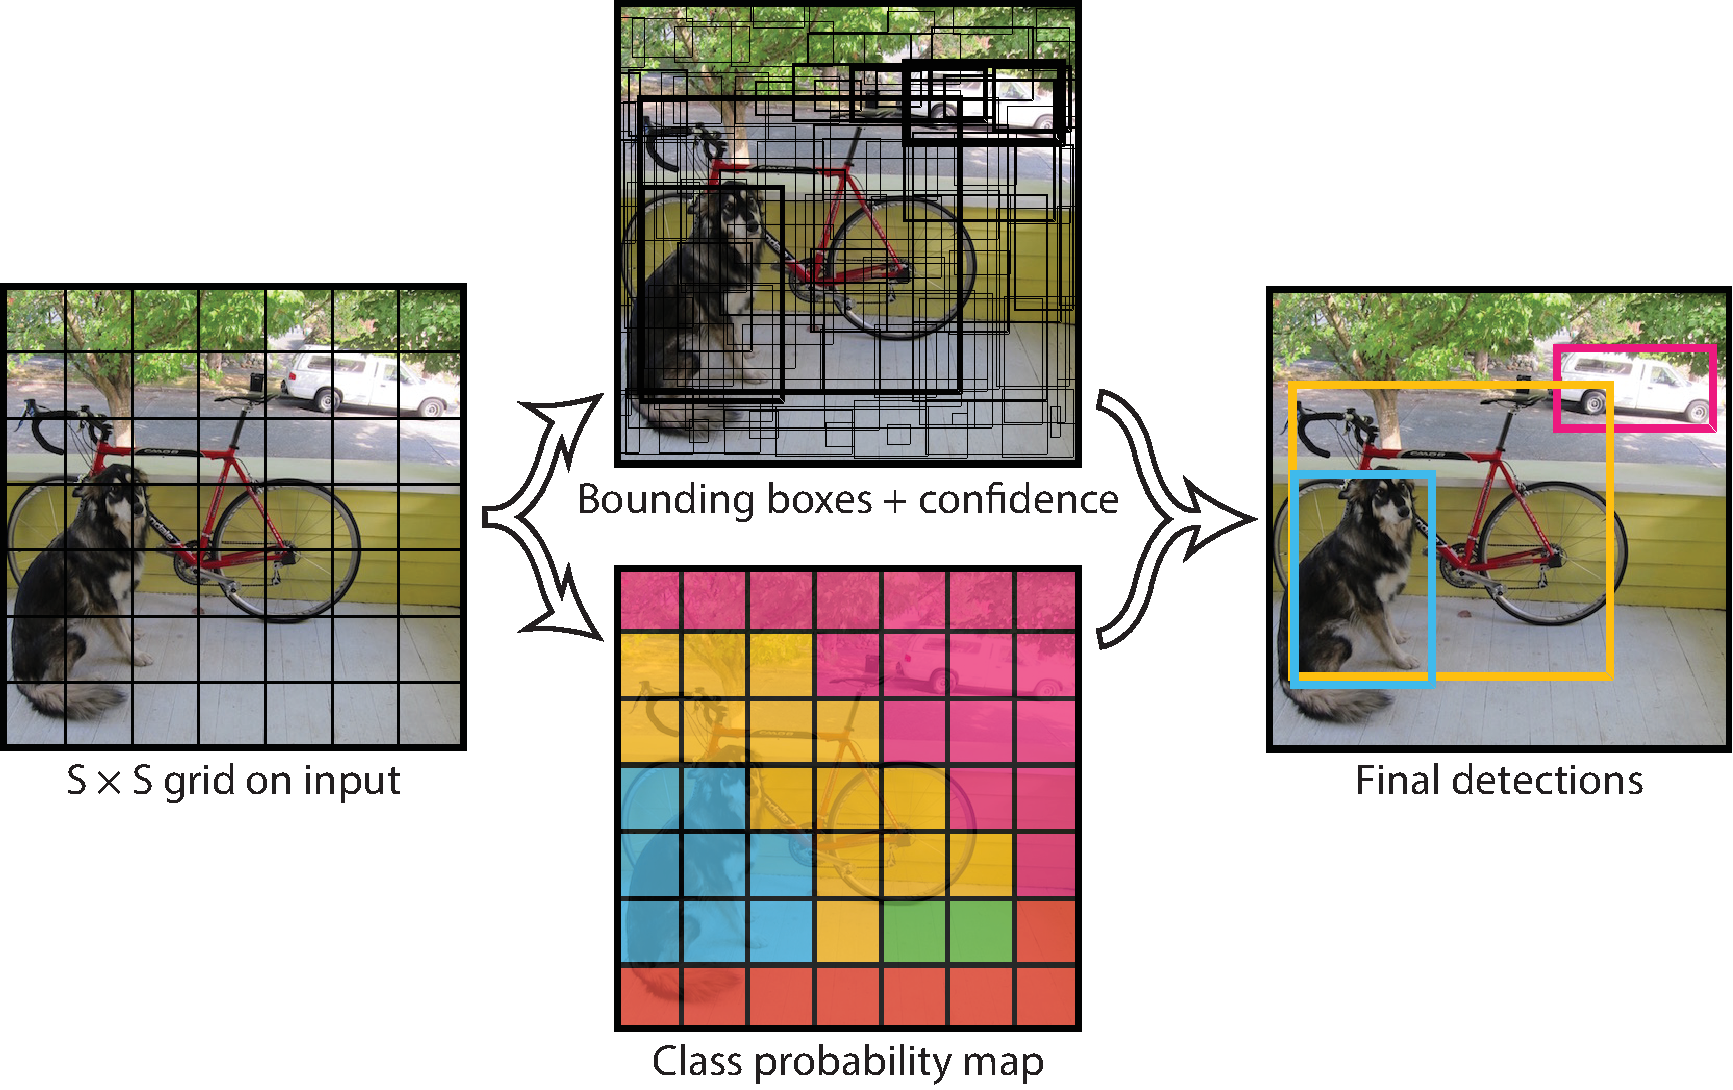
\includegraphics[width=1\linewidth]{Rohit_Master_Thesis//Images/yolo_model.pdf}
    \caption{This figure shows the working of \gls{yolo} model \cite{redmon2016you}.}
    \label{fig:yolo model}
\end{figure}

\subsubsection*{Limitations of \gls{yolo}v1 :} 

\gls{yolo} imposes significant spatial constraints on predictions of bounding box by allowing each grid cell to predict only one class and two bounding boxes. This reduces the model's ability to predict multiple nearby objects, like small objects that can appear in a group like flocks of birds \cite{redmon2016you}.

\gls{yolo} struggles when it comes to generalizing objects in new or unsual aspect ratios or configurations. Lastly, \gls{yolo}'s loss function doesn't differentiate between small and large bounding boxes. A small error in large box doesn't have much impact, but a small error in small box affects the \gls{iou}. The main cause of this problem is the \gls{yolo}'s incorrect localization \cite{redmon2016you}.

\subsection*{\gls{yolo}'s versions: }

\textbf{\gls{yolo}v2}\cite{redmon2017yolo9000}, also known as YOLO9000. It integrated several existing techniques of that time. The entire object detection architecture was converted into a full convolutional network which helps achieve high accuracy and speed. Later the high-resolution and low-resolution features are combined, and an anchor-based prediction method was adopted. Due to it's simple input and output  formats, \gls{yolo}v2 remains one of the mainly used object detection methods in maintenance and development of various industrial settings, particularly on low-end devices which has verly limited computing capabilities \cite{wang2024yolov1}.

\textbf{\gls{yolo}v3}\cite{redmon2018yolov3}, integrated advanced technology of then existing object detection and made the necessary optimizations to one-stage object detectors. \gls{yolo}v3 has architecture which combines \gls{fpn}, allowing for simultaneous predictions across multiple scales. \gls{yolo}v3 made notable changes to the label assignment task. There are two changes in the \gls{yolo}v3, the first change involves assigning a ground truth to a single anchor, and the second change involves transitioning from soft label to hard label for \gls{iou}-aware objectness. \gls{yolo}v3 is still the most popular version of \gls{yolo} series \cite{wang2024yolov1}.

\textbf{Scaled-\gls{yolo}v4} \cite{wang2021scaled}, can be used for edge and clound computing both. Due to the efforts of the DarkNet and PyTorch \gls{yolo}v3 communities, scaled-\gls{yolo}v4 is able to forgo the pre-training steps necessary with ImageNet and instead directly use a train-from-scratch method to achieve high-quality object detection outcomes. Scaled-\gls{yolo}v4 has introduced CSPNet into \gls{pan}, which significantly improves the speed, number of parameters, accuracy, and number of calculations. Scaled-\gls{yolo}v4 also introduced model scaling methods for different edge devices and offer three types of models: P5, P6, and P7. During training, it also used decoder and label assignment strategy introduced in the initial version of \gls{yolo}v5 \cite{wang2024yolov1}.

There are now many more such \gls{yolo} versions with incremental updates such as \gls{yolo}v5 \cite{yolov5}, \gls{yolo}v8 \cite{Ultralytics2024} which is used in the current solution at Siemens as mentioned in section \ref{subsec:current solution at siemens} and latest being \gls{yolo}v10 \cite{Ultralytics2024v10}.

\section{Unsupervised Image Processing}

Unsupervised image processing is also part of \gls{ml}, but unlike the supervised learning we saw in section \ref{sec:supervised}, it doesn't required any labeled data. Instead, it focuses on clustering similar data points, discovering patterns and relationships, or detecting anomalies without explicitly telling it where the defect is \cite{geeksforgeeks-sup-unsup}. This approach is beneficial when labeled data is scarce or expensive to obtain.

Below we will discuss and understand the unsupervised models we used in our experiments.

%\subsection{Anomaly Detection in Unsupervised Learning}

\subsection{PatchCore}
\label{subsec:patchcore}

PatchCore is a state-of-the-art approach developed for efficient detection of anomalies in industrial settings, especially in cases when there is a lack of defective samples or they are undefined. This approach has been specifically tailored to tackle the challenges of the cold-start problem in which models are exclusively trained on non-defective(nominal) images. PatchCore excels by utilizing a memory bank of nominal patch-features, together with techniques like locally aware patch features, and coreset subsampling which are explained below \cite{roth2022totalrecallindustrialanomaly}. Figure \ref{fig:patchcore architecture} shows the overview of the PatchCore model.

\begin{figure}[ht!]
    \centering
    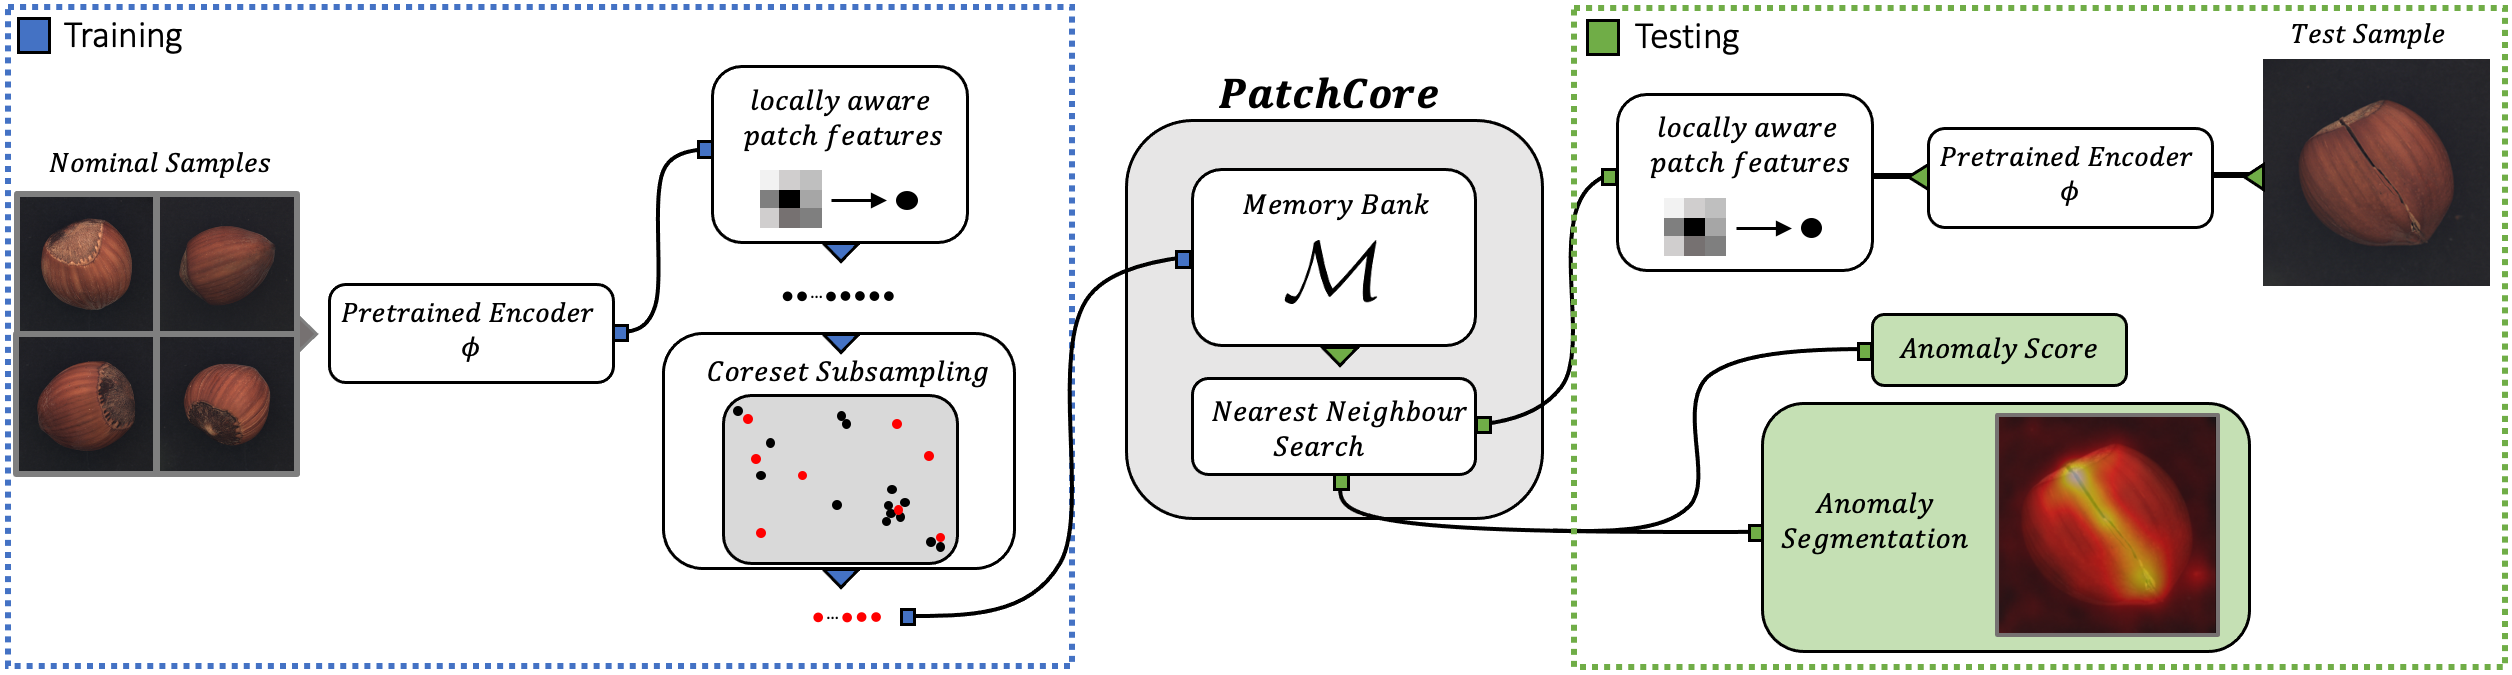
\includegraphics[width=1.1\textwidth]{Rohit_Master_Thesis//Images/patchcore_architecture_figure.png}
    \caption{Overview of PatchCore: The nominal samples are decomposed into a memory bank consisting of neighborhood-aware patch-level features. To minimize redundancy and the time required for inference, this memory bank is downsampled using greedy coreset subsampling. During the testing phase, images are classified as anomalies if there is atleast one patch is anomalous, and pixel-level anomaly segmentation is generated by assigning a score to each patch-feature \cite{roth2022totalrecallindustrialanomaly}.}
    \label{fig:patchcore architecture}
\end{figure}

\subsubsection*{Locally Aware Patch Features :} 
The key advancement of PatchCore is the utilization of locally aware patch-features. Contrary to traditional approaches that utlizes global image features, PatchCore targets local patches of the image. It extracts the mid-level features that captures the contextual and spacial relationships within these patches. By maintaining the local awareness, the model is able to preserve important details that might get lost when replying on the generalized global features \cite{roth2022totalrecallindustrialanomaly}.

The locally aware features are derived from the intermediate layers of a pre-trained \gls{cnn}, namely WideResNet-50 \cite{zagoruyko2017wideresidualnetworks}. The focus on mid-level features lets PatchCore avoid the pitfalls of over-generalization and ImageNet class bias inherent, which are common problems when relying on deeper, high-level features. The outcome is a more nuanced and contextually rich representation of the nominal data, which is essential for identifying subtle anomalies that could otherwise go unnoticed \cite{roth2022totalrecallindustrialanomaly}.

\subsubsection*{Memory Bank and Coreset Subsampling :}

PatchCores memory bank is build using these locally aware patch-features, serving as a repository of nominal patch-features, which are then used to compare against test images. however, in real-time industrial applications, a task of handling a large memory bank can be computationally expensive. In order to mitigate this issue, PatchCore uses coreset subsampling, a method that reduces the memory bank size by selecting the most representative features without compromising the model's performance \cite{roth2022totalrecallindustrialanomaly}.

Coreset subsampling employs a greedy selection algorithm, which ensures that the patches retained in the memory bank are the ones that most accurately represent the overall distribution of the nominal data. The decrease in memory bank size is essential for achieving faster inference times, also making PatchCore both accurate and highly efficient \cite{roth2022totalrecallindustrialanomaly}.

\subsubsection*{Anomaly Detection and Localization :}

During testing, PatchCore does a comparison between the patch features of a test image and the features stored in the memory bank. The Euclidean distance metric is used to compare each patch in the test image with the nearest patch in the memory bank. If any patch shows a significant deviation from the stored nominal patches, the image is flagged as anomalous. The anomaly score which serves as a robust measure for anomaly detection, is determined by calculating the maximum distance observed across all patches \cite{roth2022totalrecallindustrialanomaly}.

For the purpose of localization of anomalies, PatchCore extends this approach by creating a detailed segmentation map. A score is assigned to each patch in the test image depending on its proximity to the nearest nominal patch. These scores are subsequently mapped back to the original image, resulting in a localization map that precisely highlights the areas where the anomalies occur \cite{roth2022totalrecallindustrialanomaly}. This functionality is especially essential in industrial settings, where the ability to not only detect anomalies but also accurately determine their exact positions for quality control and remediation.

\subsubsection*{Performance and Applications :}

PatchCore has been rigorously tested across multiple benchmark datasets, such as MVTec AD dataset \cite{8954181}, where it delivered exceptional performance, achieving an \gls{auroc} of up to 99.6\%. This result marks a significant improvement over existing methods, effectively reducing detection error rates by half. Due to its ability to maintain high accuracy with minimal training data, PatchCore is especially well-suited for industrial settings where it can be difficult to gather large number of defective samples \cite{roth2022totalrecallindustrialanomaly}.

\subsection{Deep Feature Modeling (DFM)}
\label{subsec:dfm}

\gls{dfm} is an efficient method for anomaly detection, by utilizing \gls{dl} to extract feature representations and to model the distribution of normal data. This method excels in situations where the anomalies are rare and not well-defined, making it highly valuable for a range of industrial applications \cite{ahuja2019probabilisticmodelingdeepfeatures}.

The key concept of \gls{dfm} involves utilizing \gls{dnn} high-dimensional features from normal data, and subsequently modelling the distribution of these features. The assumption is that the anomalies will significantly deviate from the learned distribution, hence facilitating accurate detection. \gls{dfm} leverages the ability of \gls{dl} to automatically learn complex feature representations from raw data, in contrast to traditional methods that reply on manually crafted features \cite{ahuja2019probabilisticmodelingdeepfeatures}.

\gls{dfm} is based on the notion that the normal data can be well represented in a lower dimensional feature space, while the anomalies stands out as outliers in this space. By modeling the distribution of normal data features, \gls{dfm} can accurately identify points that deviates from the norm as anomalies \cite{ahuja2019probabilisticmodelingdeepfeatures}.

\subsubsection*{Feature Extraction and Representation :}

In \gls{dfm}, a \gls{dnn} most often a \gls{cnn} is used to extract features from the input data. These features are usually extracted from the intermediate layers of the network, which capture varying levels of abstraction, ranging from low-level edges and textures to more complex semantic information. The models performance can be greatly influenced by the choice of network architecture and the specific layer from which features are extracted \cite{8954181}.

These features are then utilized to create a feature representation space. In this space, it is expected that the normal data points will cluster together, whereas anomalies should appear distant from these clusters. To enhance visualization and anomaly detection\cite{ahuja2019probabilisticmodelingdeepfeatures}, the dimensionality of this feature space is often reduced using methods like \gls{pca}\cite{Bishop2006} or \gls{t-sne}\cite{JMLR:v9:vandermaaten08a}.

\subsubsection*{Density Estimation and Anomaly Scoring :}

\gls{dfm} uses density estimation methods to model the distribution of normal data after constructing the feature representation space during training process. Two commonly used methods for this purpose are \gls{gmm} or \gls{kde}, which are used to estimate the probability density function of normal data. The idea here is that the areas in the feature space that have a high density of normal data, whereas regions with a low concentration indicates possible anomalies \cite{ahuja2019probabilisticmodelingdeepfeatures}.

A likelihood-based anomaly score is assigned to each new data point based on its deviation from the modeled distribution. Anomalies are identified by flagging points that has a low likelihood under the modeled distribution. This method is highly effective because it doesn't require labeled data for anomalies, making it well-suited for unsupervised learning situations where only normal data is accessible during training \cite{ahuja2019probabilisticmodelingdeepfeatures}.

\subsubsection*{Anomaly Detection and Evaluation :}

During the testing phase, the trained model is given new data points to extract their feature representations. Which are then evaluated against the density model to calculate an anomaly score. Again, anomalies are identified as points for which the model assigns low likelihood \cite{ahuja2019probabilisticmodelingdeepfeatures}.

\gls{dfm} has been extensively tested on several benchmark datasets, proving its effectiveness in detecting anomalies across various domains. The evaluation of the model's performance is conducted using metrics such as the \gls{auroc}, \gls{aupr}, and accuracy. \gls{dfm} demonstrated competitive results with \gls{auroc} score of about 98\%, outperforming traditional methods for anomaly detection \cite{ahuja2019probabilisticmodelingdeepfeatures}. 

\subsection{EfficientAD}
\label{subsec:efficientad}

EfficientAD is an effective anomaly detection model for real-world computer vision application with a focus on computational efficiency and a lightweight feature extractor that can process an image in under a millisecond using a modern GPU. EfficientAD employs a \gls{s-t} approach to detect anomalous features. It establishes new standards for detecting and localizing the anomalies, coupled with its low error rate, this makes EffienctAD economical option for real-world applications \cite{batzner2024efficientadaccuratevisualanomaly}.

\subsubsection*{Core Concept :}

EffientAD sets new benchmarks for both the accuracy of anomaly detection and the speed of inference. In order to detect anomalous features, a \gls{s-t} approach is used, where the student network is trained to predict features computed by pre-trained teacher network on normal training images. EffienctAD introduces training loss that prevents the student network from imitating the teacher network beyond the normal images. This loss enables to use the efficient network architecture for both the student and the teacher, while improving the anomaly detection \cite{batzner2024efficientadaccuratevisualanomaly}. The components of EfficientAD can be divided into three main components:

1. Efficient \gls{pdn},

2. Lightweight Student-Teacher model,

3. Autoencoder for Logical Anomaly Detection,

\subsubsection*{Efficient Patch Description Network (PDN) :}

\begin{figure}[ht!]
    \centering
    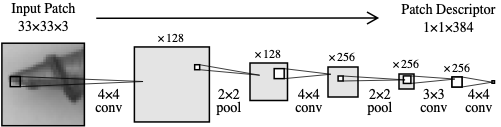
\includegraphics[width=1.1\linewidth]{Rohit_Master_Thesis//Images/pdn.png}
    \caption{\gls{pdn} architecture for EfficientAD. All features can be obtained in a single forward pass using it on an image in a fully convolutional manner \cite{batzner2024efficientadaccuratevisualanomaly}.}
    \label{fig:pdn architecture}
\end{figure}

Recent anomaly detection methods often employs deep pretrained networks for feature extraction. EffienctAD employs a feature extractor network of drastically reduced depth. This festure extractor is referred to as \gls{pdn}, its architecture as shown in figure \ref{fig:pdn architecture} contains only four convolutional layers. The receptive field of each output neuron is $33\times33$ pixels, which makes \gls{pdn} possible to generate all feature vectors in a single forward pass for images of different sizes \cite{batzner2024efficientadaccuratevisualanomaly}.

To overcome the large feature maps size, high computational costs and memory requirement problems, \gls{pdn} performs early stage downsampling by strided average-pooling layers after the first and second convolutional layers as shown in figure \ref{fig:pdn architecture}. To generate expressive features, \gls{pdn} is trained by distilling a deep pretrained classification network into it. \gls{pdn} trained in images from ImageNet by reducing the mean squared difference between its output and the features extracted from the pretrained network. Besides higher efficiency, this has another benefit that the features generated by \gls{pdn} only depends on local pixels. avoiding long-range dependencies in other methods. This ensures that an anomaly detected in one area of the image can't activate anomalous feature vectors in other distant areas, which can compromise the localization of anomalies \cite{batzner2024efficientadaccuratevisualanomaly}.

\subsubsection*{Lightweight Student-Teacher model :}

For anomalous feature vectors detection, EfficientAD uses a \gls{s-t} approach, with teacher being the \gls{pdn}. The student network uses the teachers architecture as well to maintain low overall latency. EfficientAD model introduces a training loss  which substantially improves the anomaly detection without affecting the test time computational requirements. The goal is to provide the student with enough data so that it can mimic the teacher on normal images, while avoiding generalization on anomalous images. Therefore the student's loss is restricted to the most relevant parts of an image i.e. the patches where the student mimics the teacher the least.A hard feature loss is proposed, which primarily uses the output elements with the highest loss for the purpose of backpropagation \cite{batzner2024efficientadaccuratevisualanomaly}.

Apart form hard feature loss, EfficientAD adds a loss penalty during training that further hinders the student's ability from imitating the teacher on images that are not included in the normal training images. The teacher network is either pretrained on image classification dataset, or is a distilled version of a pretrained network, but student is only trained on the applications normal images. To hinder the student's ability to generalize its imitation of the teacher to out-of-distribution images, a penalty in terms of using images from the teacher's pretraining during the training of student is proposed \cite{batzner2024efficientadaccuratevisualanomaly}.

\subsubsection*{Autoencoder for Logical Anomaly Detection :}

For learning logical anomalies of the training images and detecting any violations of these constraints, EfficientAD uses autoencoder on training images. Figure \ref{fig:EfficientAD pipeline} illustrates the anomaly detection pipeline for EfficientAD. It consists of \gls{s-t} pair and an autoencoder. The autoencoder is trained to predict teacher's output. A standard convolutional autoencoder is used, that consists of strided convolutions in the encoder and bilinear upsampling in the decoder \cite{batzner2024efficientadaccuratevisualanomaly}.

Usually for both the logical anomalies as well as normal images, the autoencoder fails to generate accurate latent code needed for reconstruction of the image in the teacher's feature space as can be seen in the figure \ref{fig:EfficientAD pipeline}. By using the difference the teacher's output and the autoencoder's reconstruction as an anomaly map might cause false-positive detections. To avoid this, student's output channels are doubled, and is trained to predict the output of the autoencoder in addition to the output of the teacher \cite{batzner2024efficientadaccuratevisualanomaly}.

\begin{figure}[ht!]
    \centering
    \includegraphics[width=1.1\linewidth]{Rohit_Master_Thesis/Images/efficientAD_pipeline.pdf}
    \caption{EfficientAD pipeline}
    \label{fig:EfficientAD pipeline}
\end{figure}

The student learns the systematic reconstruction errors of the autoencoder on normal images, but it doesn't learn the reconstruction errors for anomalies as they are not part of the training set. This makes the difference between the student's and the autoencoder's output suitable for computing the anomaly map, which is calculated as squared difference between the two outputs and then averaging across all channels. EfficientAD produces two anomaly maps, the one generated by autoencoder-student pair is called global anomaly map and the one generated by \gls{s-t} pair is called local anomaly map as seen in the figure \ref{fig:EfficientAD pipeline}. Then these two maps are normalized to similar scale and then averaged to generate the combined anomaly map, and its maximum value is used as image-level anomaly score \cite{batzner2024efficientadaccuratevisualanomaly}.

\subsubsection*{Performance :}

EfficientAD achieves an impressive image-level \gls{auroc} score of $99.8\%$ on MVTec AD dataset\cite{8954181} with early stopping enabled. For the overall anomaly detection performance, EfficientAD achieves very strong image-level detection and pixel-level localization performance with a highest score of $98.1$ for VisA\cite{zou2022spotthedifferenceselfsupervisedpretraininganomaly} dataset. The computational cost of EfficientAD was measured using the metrics latency and throughput, with the EfficientAD showing latency of $2.2ms$ and throughput of 614 $img/s$ \cite{batzner2024efficientadaccuratevisualanomaly}.

\subsection{FastFlow}
\label{subsec:fastflow}

Most existing representation-based moethods uses a deep convolutional neural network to extract normal image features and are then characterized this distribution through non-parametric distribution estimation methods. But these methods fails to map features effectively to a tractable base distribution and ignore the relationship between the local and global features which are essential for anomaly detection. Therefore, FastFlow is proposed to mitigate these problems. FastFlow is an unsupervised anomaly detection and localization model which is built with 2D normalization flows as its probability distribution estimator. Experimental findings shows that FastFlow outperforms previous state-of-the-art methods in terms of both accuracy and inference efficiency. It achieves 99.4\% AUC in anomaly detection \cite{yu2021fastflowunsupervisedanomalydetection}.

\subsubsection*{Core Concept :}

Earlier unsupervised approaches used non-parametric methods while recents ones started using normalization flow to model the distribution of features for normal images. However these one-dimensional normalization flow models  requires the flattening of the two-dimensional input feature into a one-dimensional vector to estimate the distribution which destroys the positional relationship of 2D image and limits the ability of flow model. These models also used sliding window approach to extract features from a large number image patches and detect anomalies for each patch, this led to high inference complexity. Therefore to address the above problems FastFlow which extends the normalizing flow to two-dimensional space by using fully connected neural networks as the subnet which can maintain the relative position of the space, and supports end-to-end inference of the whole image. This improves the anomaly detection performances and gives the detection and localization results at once for the whole image to improve inference efficiency \cite{yu2021fastflowunsupervisedanomalydetection}.

\begin{figure}[ht!]
    \centering
    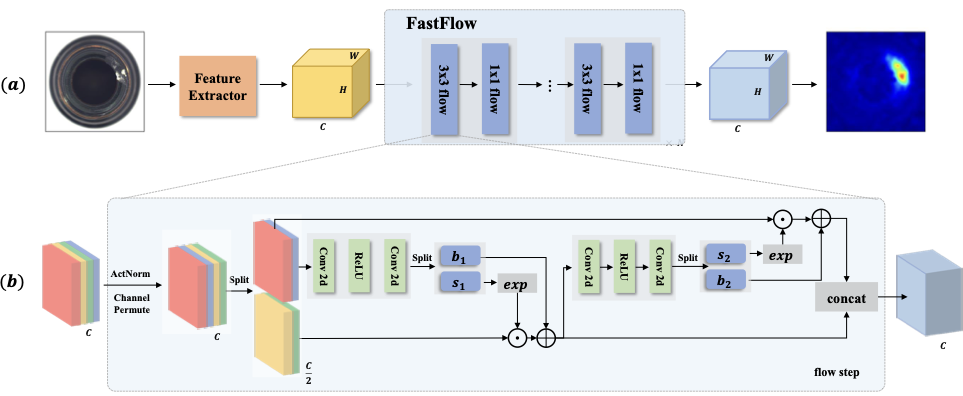
\includegraphics[width=1.1\linewidth]{Rohit_Master_Thesis//Images/fastflow_pipeline.png}
    \caption{FastFlow pipeline\cite{yu2021fastflowunsupervisedanomalydetection}}
    \label{fig:fastflow pipeline}
\end{figure}

Figure \ref{fig:fastflow pipeline} shows the FastFlow pipeline, in which first the visual features are extracted using the feature extractor and then passed as an input to the FastFlow module for probability density estimation. During training FastFlow is trained using normal images to convert the normal distribution into a standard normal distribution in 2D manner. For inferencing, anomaly score is assigned  to each location on the two-dimensional feature based on its probability values \cite{yu2021fastflowunsupervisedanomalydetection}.

The FastFlow pipeline consists of two main components, they are:

1. Feature Extractor,

2. 2D Normalization Flow

\subsubsection*{Feature Extractor :}

First step in the whole pipeline is to extract representative features from input image using either ResNet as explained in section \ref{subsec:ResNet} or \gls{vit}. In \glspl{vit} as feature extractor, features from only one layer are extracted because of its capability to capture the relationship between local patches and global features. In case of ResNet, features are taken from directly the last layer in the first three blocks, and then these features are inputted into three corresponding FastFlow model \cite{yu2021fastflowunsupervisedanomalydetection}. 

\subsubsection*{2D Normalization Flow :}

The 2D flow function is used to project the image features into the hidden variable using a bijective invertible mapping. At the time of inference, the features of anomalous images should be out of distribution and therefore will have lower likelihoods than normal images. This likelihood can be use as the anomaly score. Secifically, the sum of 2D probabilities of each channel is done to obtain the final probability map, and then its upsampled to the input image resolution using bilinear interpolation. In order to convert the original normalization flow into a 2D format, an alternate $3\times3$ and $1\times1$ convolutional layers are used in the default subnet as shown in the figure\ref{fig:fastflow pipeline} to retain the spatial information in the flow model and the loIn the feature extraction stage, the features are extracted using \gls{dnn} as the backbone, such as ResNet[mention reference], which was pre-trained on ImageNet\cite{5206848} dataset \cite{10208786}., CIFAR-10\cite{krizhevsky2009learning}, BTAD\cite{Mishra_2021} datasets. For MVTec AD dataset, the FastFlow model was compared with many state-of-the-art models with two metrics image-level \gls{auc} and pixel-level \gls{auc}. FastFlow demonstrates exceptional performance in anomaly detection, achieving an 99.4 image-level \gls{auc}, and 98.5 pixel-level \gls{auc}, surpassing all the other models. In case of CIFAR-10 dataset, FastFlow achieves an \gls{auc} 66.7 which is the best performing model when compared with others. For the BTAD dataset, FastFlow again surpasses all the compared models and achieves a pixel-level \gls{auc} of 97.0 \cite{yu2021fastflowunsupervisedanomalydetection}.

\subsection{Deep Feature Kernel Density Estimation (DFKDE)}
\label{subsec:dfkde}

\gls{dfkde} is a fast one-class anomaly detection model. It consists of two stages:

1. Feature extraction stage,

2. Anomaly detection stage,

In the feature extraction stage, the features are extracted using \gls{dnn} as the backbone, such as ResNet[mention reference], which was pre-trained on ImageNet\cite{5206848} dataset \cite{10208786}. The penultimate layer which is the average pooling layer of the backbone is used to obtain a semantic feature vector of a fixed length of 2048 \cite{Anomalib2024}.

In the anomaly detection stage, once the features are extracted, then these features undergoes dimensionality reduction using \gls{pca}\cite{IBM2023} to get the first 16 principal components. \gls{pca} is among the simple and most straightforward ways of doing dimensionality reduction. Its a technique that reduces high-dimensional data into a lower-dimensional representation by using the dependencies between variables, without loosing too much information \cite{Shalizi2012}. After the features are reduced using \gls{pca}, then on these reduced features Gaussian \gls{kde} is applied. The main idea behind \gls{kde} is that the training datasets will follows some random distribution, and this distribution can be modelled by employing \gls{kde} \cite{10208786}.

During inference, if a lower probability density is observed below the threshold determined by the training dataset, this indicates the existence of an anomaly compared the data distribution learned from the training data \cite{10208786}. The \gls{dfkde} gives competitive results on MVTec AD\cite{8954181}, for the metric \gls{auroc} \gls{dfkde} gives highest of 96.5 score \cite{Anomalib2024}.

\textbf{see if I want to write about densenet, DeiT, CaiT architectures in the theory section.}

   % (\chapter{})
\clearpage
\chapter{Methods}

This section provides an outline of the actual experimental procedures and processes carried out to conduct the research study. It includes datasets, the process of training and testing the model, and metrics used to evaluate the method's performance.

\section{Dataset}
The dataset provided by Siemens consists of images of Solder joints on a \gls{pcb}. It has a total of 6014 images, each of $512 \times $512 dimensions, divided into \gls{fc} and \gls{ng}. The \gls{fc} class contains images without defects, while the \gls{ng} class contains images with a variety of defects. The images are of two types, one is colored image as shown in middle of figure\ref{fig:dataset-FC}, and other is heat image which are the red ones in figure\ref{fig:dataset-FC}. This variation of images makes it suitable for evaluating variety of images a model can be used for. The dataset is split into training and testing sets using an 80-20 split. A separate set of 160 images is also reserved for testing, finding accuracy and visualizing classification and segmentation results.

\begin{figure}[ht!]
    \centering  
    \begin{minipage}{0.32\textwidth}
        \centering
        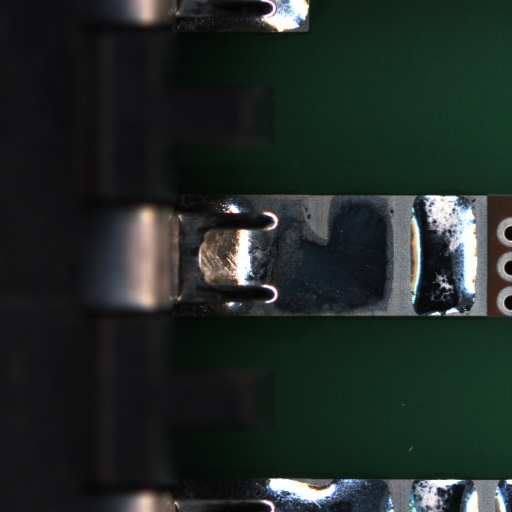
\includegraphics[width=\textwidth]{Images/Val_NG_BF2003043437_151_7_816_816_Color_origin.jpg} % Add your image file name here
        %\caption{An example of a defective piece of leather.}
    \end{minipage}
    \begin{minipage}{0.32\textwidth}
        \centering
        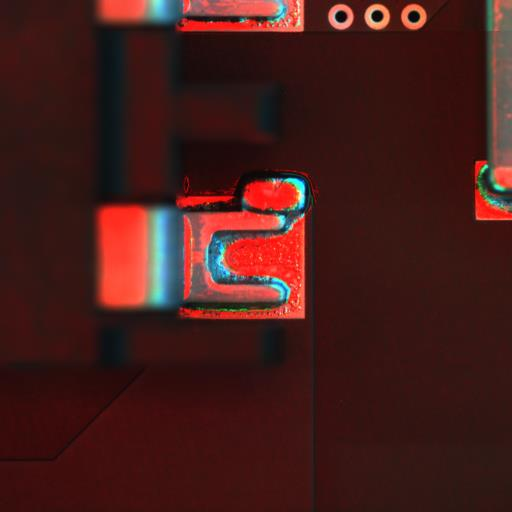
\includegraphics[width=\textwidth]{Images/Val_NG_BF2003033542_223_32_471_471_Multi_origin.jpg} % Add your image file name here
        %\caption{An example of a defective grid.}
    \end{minipage}\hfill
    \caption{Examples of defective solder joints in the dataset.}
    \label{fig:dataset-NG}
\end{figure}

\begin{figure}[ht!]
    \centering
    \begin{minipage}{0.32\textwidth}
        \centering
        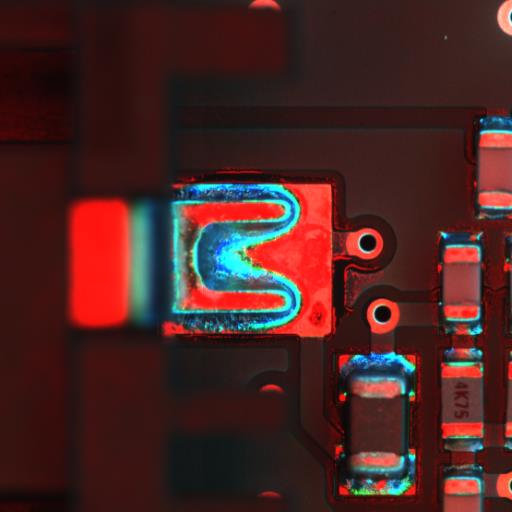
\includegraphics[width=\textwidth]{Images/Val_FC_heat_BF2003054784_4796_144_2042_2042_Multi.jpg} % Add your image file name here
        %\caption{An example of a defective tile.}
    \end{minipage}   
    \begin{minipage}{0.32\textwidth}
        \centering
        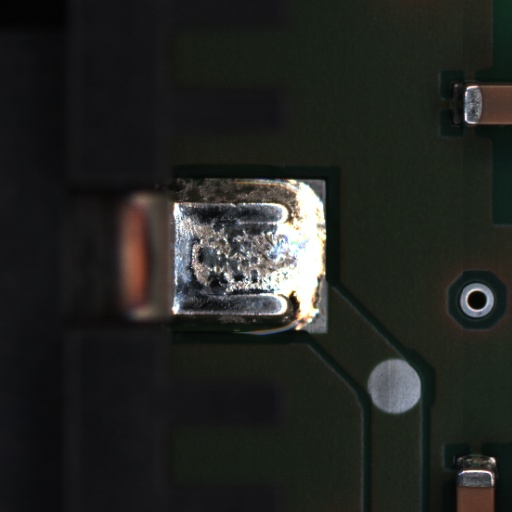
\includegraphics[width=\textwidth]{Images/train_FC_BF2003015014_1174_42_2038_2038_Color.jpg} % Add your image file name here
        %\caption{An example of a defective piece of leather.}
    \end{minipage}\hfill
    \caption{Examples of defect-free solder joints in the dataset.}
    \label{fig:dataset-FC}
\end{figure}

As can be seen in the figure \ref{fig:dataset-NG}, and figure \ref{fig:dataset-FC} finding a defect without expertise can be challenging and time-consuming.

The table~\ref{tab:dataset-distribution} provides a detailed breakdown of the dataset distribution across subsets:

\begin{table}[ht!]
    \centering
    \begin{tabular}{|l|c|c|c|}
        \hline
        \textbf{Dataset} & \textbf{FC (No Defects)} & \textbf{NG (Defective)} & \textbf{Total} \\
        \hline
        Training & 2,971 & 1,712 & 4,683 \\
        \hline
        Testing & 743 & 428 & 1,171 \\
        \hline
        Custom Test & 80 & 80 & 160 \\
        \hline
    \end{tabular}
    \caption{Distribution of Images in the Dataset}
    \label{tab:dataset-distribution}
\end{table}

\section{Experiment}

Experiments were carried out using models mentioned in the [Theory section]. All the models belongs to Anomaly detection and are part of a deep learning library which has a collection of state-of-the-art anomaly detection algorithms call Anomalib. There are multiple steps taken in this experiment and they will be explained below.

\subsection{Data Loading}

To load and preprocess our dataset, we use Anomalib dataloader by importing \textbf{Folder} from \textbf{Data} class which is specifically designed for handling our custom dataset, allowing for efficient data management and preprocessing. We create a Folder datamodule and configure several parameters as described below.

\textbf{Name :} It is designated as the dataset configuration identifier, reflecting the specific dataset used for the particular experiment.

\textbf{Root Directory :} It points to the directory containing the organized dataset folders.

\textbf{Normal \& Abnormal Directories :} Models mostly requires anomalous free images for training which in our case is \gls{fc}, and anomalous images for testing(not used while training) which is \gls{ng}. So those are provided in these two fields.

\textbf{Normal Split Ratio :} The datamodule employs a 0.2 split ratio for validation of normal images, which ensures a sufficient number of samples for model tuning and validation.

\textbf{Image Size :} All images are resized to $256 \times 256$ pixels during preprocessing, balancing the need for detailed feature representation with computational efficiency.

\textbf{Batch Size :} Both training and evaluation processes uses different batch sizes for different models explained in [chapter 2] to optimize \gls{gpu} memory usage while maintaining effective gradient updates.

\textbf{Task Type :} There are two types of tasks available, one is Classification and other one is Segmentation. For this thesis for all the model we have set the parameter to "CLASSIFICATION" and it directs the model to perform binary classification between the \gls{fc} and \gls{ng} categories.

\textbf{Number of Workers :} Based on the \gls{gpu} and the model being used the number of workers varied between 0 to 8 for helping the computational resources to parallelize data loading.


%\subsubsection{Model Loading}

Model loading is carried out by importing Here each model is configured with a specific backbone, which serves as a feature extraction component. 

\subsection{Model Training or Inferencing}
\label{subsec:Model Training}

The training takes place in two steps here, first is loading the model, second is the training part, which are explained below.

\textbf{Model Loading :} Firstly model of our choice is imported, the models used in this thesis are explained in [3nd section]. Each model is initialized with a specific backbone, such as '\gls{resnet}18', '\gls{resnet}50', 'Wide\gls{resnet}50' etc. These backbones are critical for feature extraction. The selection of backbone and the specific layers used for feature extraction are the key factors that influence the model's ability to detect anomalies.

\textbf{Model Training or Inferencing :} Once the model is loaded, next steps involves training or inferencing using the \textbf{Engine} class from Anomalib. Depending on the model we need to either train the model or just perform inferencing(extracting the features). The engine is configured to manage the complete process, ensuring that the model is trained effectively and can accurately infer from the data provided.

The key components of training/inferencing configuration are:

\textbf{Thresholding :} Threshold value is used to determine the anomalous label for the calculated anomaly scores. There are two types of thresholding methods available, one is '\textbf{ManualThreshold}' where we have to set our own threshold value, this is beneficial in situations where there is a lack of appropriate representative validation data\cite{9897283}. Second one which we have used is '\textbf{F1AdaptiveThreshold}'. The algorithm optimizes the value of threshold to determine the optimal f1\_score and saves the calculated value of the adaptive threshold.\cite{Anomalib2024}

\textbf{Task Type :} The task is usually set to '\textbf{CLASSIFICATION}', which directs the model to categorize images into predefined classes (ex., normal, and anomalous). Depending on the requirements, task can also be configured to '\textbf{SEGMENTATION}' for pin point where the defect is there in the image.

\textbf{Image Metrics :} The model's performance is evaluated by '\textbf{\gls{auroc}}' and '\textbf{F1Score}'. They are standard metrics used for assessing classification accuracy and balance between precision and recall. These metrics will be explained in detail in section \ref{subsec:Evaluation Metrics}.

\textbf{Accelerator :} Depending on the available resources, the engine can run on a \textbf{'\gls{gpu}'}, \textbf{'\gls{cpu}'}, \textbf{'\gls{tpu}'}, \textbf{'\gls{ipu}'}, also there is an \textbf{'auto'} which chooses the appropriate resource automatically based on the availability.

\textbf{Devices :} This configuration allows for us to provide the engine the available number of devices(ex., \glspl{cpu}, \glspl{gpu}) to use during training and inference. The \textbf{'auto'} option sets the optimal devices automatically for the engine.

\textbf{Validation Frequency :} This option is used for validating the model after every epoch \textbf{'check\_val\_every\_n\_epoch=1'}, ensuring that the performance metrices are tracked throughout the training process.

\textbf{Max Epochs :} Depending on the model we are using it can either required to be trained or do inferencing on. When the model is performing inferencing at that time the \textbf{'max\_epochs'} parameter is always set to \textbf{1}. And for the models requiring training can be adjusted depending on the complexity of the model.%might need to add more info.

\textbf{Validation Check Interval :} The parameter \textbf{'val\_chedck\_interval'} sets when the validation checks are performed, in our case its set to \textbf{1.0} meaning the validation checks are performed after every epoch.

After providing these training configuration to the engine class, then we can call the \textbf{fit} function to start with the training or inferencing. Here we provide the model and the datamodule components. Here the \textbf{Normal} directory is used which is the anomaly free images. After the training/inferencing is finished, the next step is to perform testing which is explained in below section.

\subsection{Testing}

After the training/inferencing is finished, we can move ahead to next critical step i.e. to evaluate the model's performance. For this the \textbf{test} function from the engine class is used, and similar to fit function we again need to pass the model and the datamodule components. Here the \textbf{Abnormal} directory is used which has the anomalous images. 

After the testing is finished, its results are displayed which have two of the metrics mentioned in section \ref{subsec:Evaluation Metrics} \gls{auroc} and F1-Score.

\subsection{Model Exporting}
\label{subsec:Model Exporting}

Exporting a trained model is a very important task, as then the model can be deployed in real-world applications. This involves converting the trained model into a format optimized for efficient inference on various hardwares, like \glspl{cpu}, \glspl{gpu} etc. Thus the model can be incorporated into production environments, operating at scale by processing new data and identifying anomalies in real-time.

The Anomalib library lets us convert the models into formats like OpenVINO, ONNX etc. We are exporting our models into OpenVINO format. OpenVINO is a open-source software toolkit used to optimize and deploy \gls{dl} models. It minimizes resource requirements and effectively deploy on various platforms like cloud. OpenVINO\textsuperscript{TM} enables inference on several hardware platforms, including \glspl{cpu}, \glspl{gpu}.\cite{openvino2024}

The export process is initialized by setting the desired export format via the \textbf{'ExportType'} variable. The trained model and the destination where the model should be exported are then passed to the \textbf{'Export'} function present in the engine class, which is responsible for the conversion. In the specified export location, three files are save there:

\textbf{1. 'metadata.json'} which stores the threshold value as mentioned in the section \ref{subsec:Model Training} based on which the classification can be done.

\textbf{2. 'model.bin'} its a binary file that contains the weights and biases of the model.

\textbf{3. 'model.xml'} this file stores the models architecture. It contains the structure of neural network, including layers, the connections between them etc.

\section{Inference}
\label{subsec:Inference}

In the inference phase the model is utilized to make predictions on new and unseen data. This section documents the approaches for achieving inference using a trained model, mainly focusing on two tasks: \textbf{'Image Classification'} and \textbf{'Image Segmentation'}. Both the tasks are crucial in assessing the effectiveness of the model in detecting and localizing anomalies in solder joints on \glspl{pcb}.

Firstly the trained model is loaded using the \textbf{'OpenVINOInferencer'} or \textbf{'TorchInferencer'} class which can enable efficient inference on \glspl{cpu} or \glspl{gpu} respectively. Here we will be using OpenVINOInferencer, by providing the model and metadata paths of the trained model as explained in the section \ref{subsec:Model Exporting}. Once we are done with creating the \textbf{'Inferencer'} object, then we can move on to performing image classification and segmentation as described below.

\subsection{Image Classification}
\label{subsec:Image Classification}

Image Classification is an important task within \gls{cv} because it helps in identifying and recognizing the object present in an image. It involves labelling input images based on the likelihood of it being anomalous or not \cite{FANG2020100980}.

As mentioned in section \ref{subsec:Inference}, after creating the inference object then we pass the input image to its \textbf{'predict'} function, which calculates the predicted label and the anomalous score. The predicted results are then visualized using \textbf{'ImageVisualizer'} class, its configured for \textbf{CLASSIFICATION} mode, so it overlays the classification results on the input image, making it simpler to analyze the results.

\begin{figure}[ht!]
    \centering
    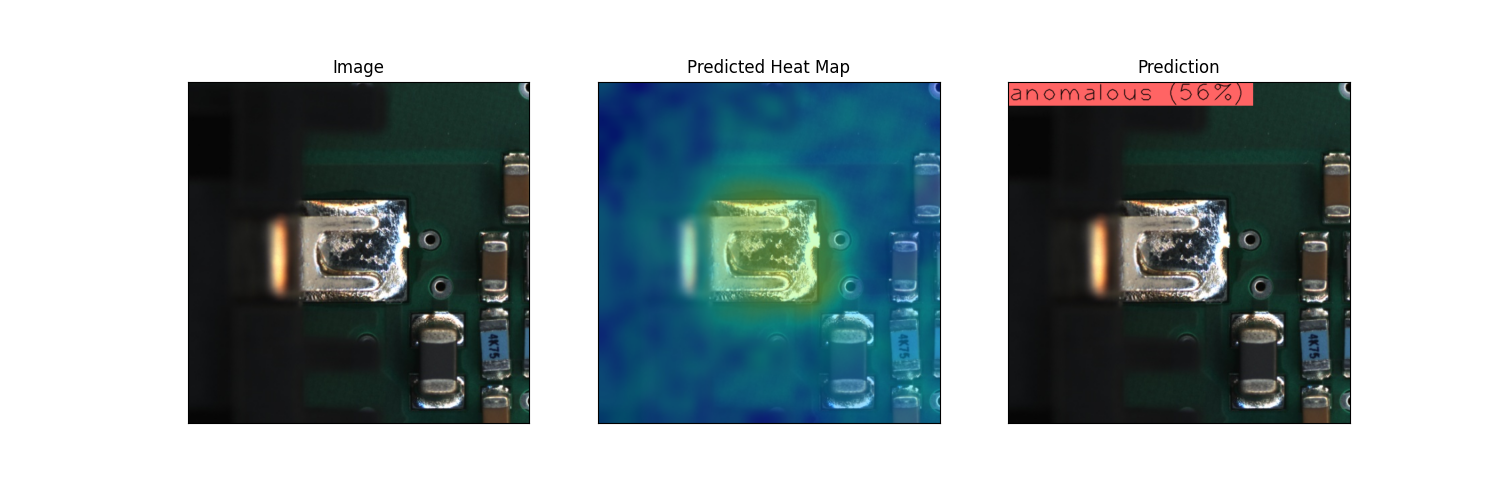
\includegraphics[width=1\linewidth]{Images/anomalous_image_classification.jpg}
    \caption{Image Classification on NG image}
    \label{fig:Image classification on NG image}
\end{figure}

The figure \ref{fig:Image classification on NG image} shows the result of image classification, where it gives three images as an output, one is the input image, second one shows the predicted heat map which shows where could be the possible anomaly, and the third gives the prediction label and the score.

\subsection{Image Segmentation}
%\subsubsection{Metrics Calculation}

Image segmentation is a method of analyzing images at the pixel level. It involves utilizing multiple techniques to label each pixel as part of a particular class or instance\cite{IBM2024}. So using image segmentation we can we can point where the model has predicted the anomaly to be as shown in the figure \ref{fig:Image Segmentation on NG image}.

\begin{figure}[ht!]
    \centering
    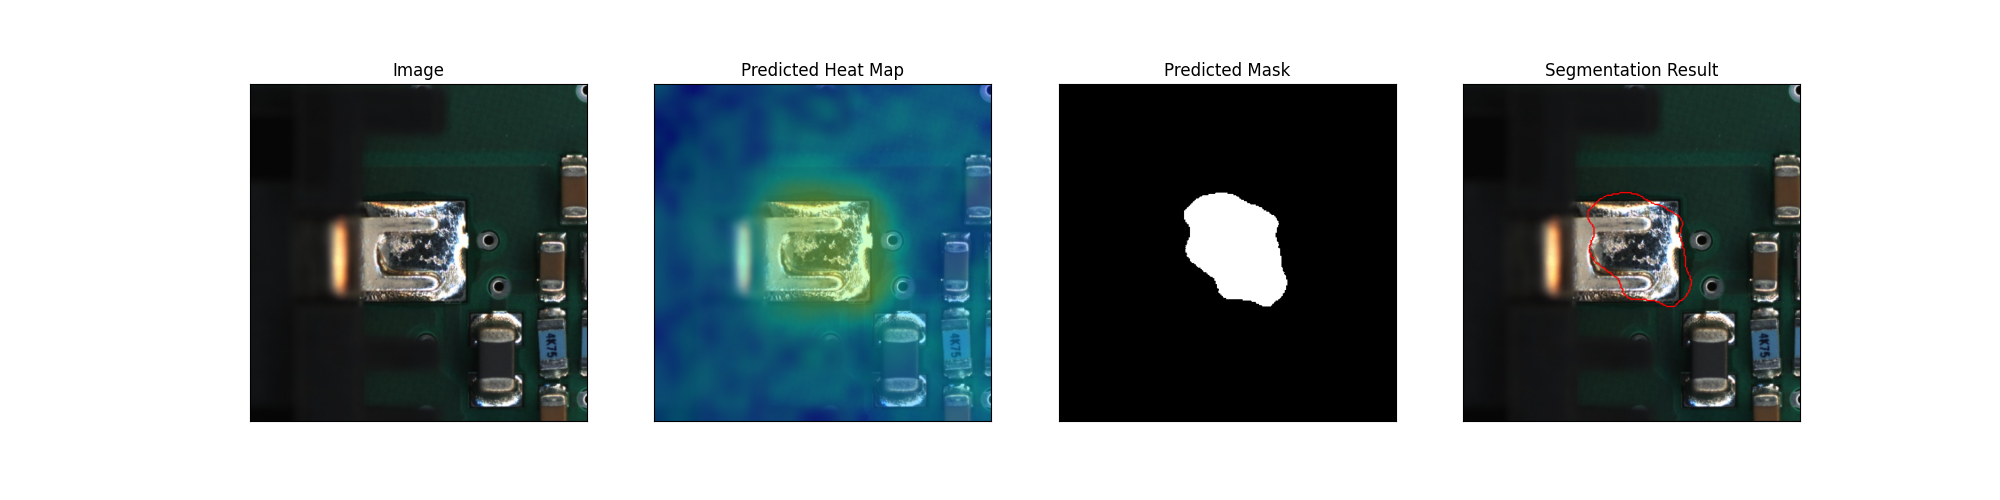
\includegraphics[width=1\linewidth]{Images/anomalous_image_segmentation.jpg}
    \caption{Image Segmentation on NG image}
    \label{fig:Image Segmentation on NG image}
\end{figure}

\section{Evaluation Metrics}
\label{subsec:Evaluation Metrics}

Evaluation metrics play a crucial role in assessing the performance of a machine learning model. These metrics aid in quantifying the model's ability to differentiate between anomalous and normal images, offering valuable insights into the model's effectiveness and areas that can be improved. This section outlines the primary evaluation metrics utilized in this thesis: AUROC, Accuracy, Recall, Precision, F1-Score, and Confusion Matrix.

\subsection*{Area Under the Receiver-Operating Curve (AUROC)}
\label{subsec:AUROC}

The \gls{auroc} measures the ability of a classification model to differentiate across different classes. It has been particularly useful in measuring trade-offs of the \gls{tpr} (sensitivity) versus the \gls{fpr} (1-specificity) across different threshold settings. A higher \gls{auroc} value indicates better model performance, with a value of 1 representing a perfect model and a value of 0.5 indicating a model that performs no better than random chance\cite{FAWCETT2006861}. For quality control applications, this is extremely important because, missing an anomaly can possibly have severe consequences for a manufacturing process. %Write how its calculated in anomalib if possible

\subsection*{Accuracy}
\label{subsec:Accuracy}

Accuracy is the rate of correct predictions made by the model. It is often assessed by using an unseen dataset that was never utilized throughout the learning process, like the custom test set mentioned in the table \ref{tab:dataset-distribution}.\cite{Kohavi1998}. It is expressed as: 

\begin{equation}
    \text{Accuracy} = \frac{\text{\gls{tp}} + \text{\gls{tn}}}{\text{\gls{tp}} + \text{\gls{tn}} + \text{\gls{fp}} + \text{\gls{fn}}} \quad \text{\cite{Walker2024}}
    \label{eq:accuracy}
\end{equation}

where \gls{tp}, \gls{tn}, \gls{fp}, and \gls{fn} are True Positives, True Negatives, False Positives, and False Negatives, respectively. It gives an overall view of the performance of the model.

\subsection*{Recall}
\label{subsec:Recall}

Recall, also known as sensitivity, refers to the ratio of accurately predicted positive cases to the total number of actual positive cases \cite{powers2020evaluationprecisionrecallfmeasure}. It is expressed as:

\begin{equation}
    \text{Recall} = \frac{\text{\gls{tp}}}{\gls{tp} + \gls{fn}} \quad \text{\cite{powers2020evaluationprecisionrecallfmeasure}}
    \label{eq:recall}
\end{equation}

A higher Recall value means that the model is good in detecting most anomalies, but it doesn't take into account the number of \gls{fp}.

\subsection*{Precision}
\label{subsec:Precision}

Precision, also known as confidence, refers to the proportion of accurately predicted positive cases that are actually correct \cite{powers2020evaluationprecisionrecallfmeasure}. It is expressed as:

\begin{equation}
    \text{Precision} = \frac{\text{\gls{tp}}}{\gls{tp} + \gls{fp}} \quad \text{\cite{powers2020evaluationprecisionrecallfmeasure}}
    \label{eq:precision}
\end{equation}

This metric is very important where the cost of false positives is high, because it indicates how well the model can prevent incorrectly labelling normal cases as anomalies. 

\subsection*{F1-Score}
\label{subsec:F1-Score}

The F1-score is a metric that achieves a balance between precision and recall. The calculation involves taking the harmonic mean of precision and recall. The F1-score is a valuable metric for achieving a trade-off between high precision and recall. It effectively penalizes extreme negative values of either component \cite{Walker2024}. It is expressed as:

\begin{equation}
\text{F1-Score} = 2 \times \frac{\text{Precision} \times \text{Recall}}{\text{Precision} + \text{Recall}} \quad \text{\cite{Walker2024}}
\end{equation}

It makes this metric valuable since it evaluates the ability of a model to detect anomalies(Recall) and  its precision identifying true positives without an excessive number of false positive. 

\subsection*{Confusion Matrix}
\label{subsec:Confusion Matrix}

Confusion Matrix is a matrix which simply shows the predicted and the actual classifications made by the model \cite{Kohavi1998}. It is basically a table containing the \gls{tp}, \gls{tn}, \gls{fp}, and \gls{fn} values. Subsequently, a Confusion Matrix can help to explain what kinds of errors a model makes so that improvements can be made specifically within the same area.

\begin{figure}[ht!]
    \centering
    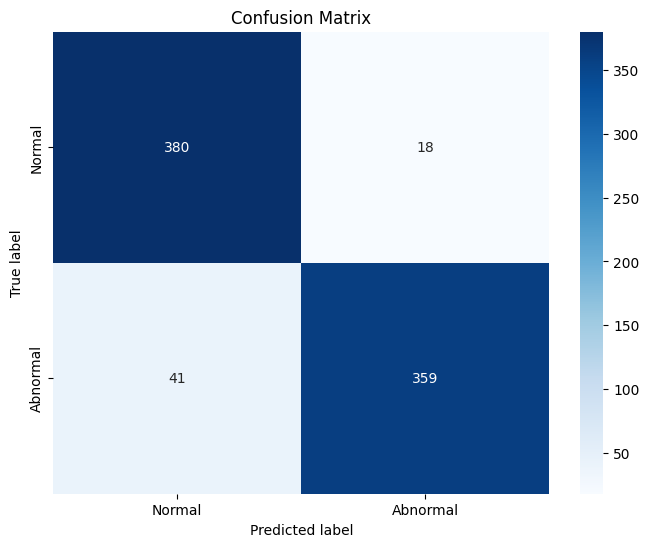
\includegraphics[width=1\linewidth]{Images/confusion matrix.png}
    \caption{Example of Confusion Matrix}
    \label{fig:confusion matrix}
\end{figure}

The figure \ref{fig:confusion matrix} shows a confusion matrix from one of our model. Here the \gls{tp} is the top-left corner dark blue cell, \gls{tn} is the bottom-right dark blue cell, \gls{fp} is the bottom-left light blue cell, and \gls{fn} is the upper-right light blue cell.



\clearpage
\chapter{Results}

This section presents the detailed findings and results of our experiments using various unsupervised anomaly detection models for the task of identifying faulty solder joints in \gls{pcb}. The models which we have evaluated here are PatchCore(section \ref{subsec:patchcore}), \gls{dfm}(section \ref{subsec:dfm}), \gls{dfkde}(section \ref{subsec:dfkde}), EfficientAD(section \ref{subsec:efficientad}), FastFlow(section \ref{subsec:fastflow}), which uses different hyperparameters, feature extraction backbones and its layers. We aim to study the effectiveness of these models in comparison to the current baseline models used by Siemens \gls{yolo}(section \ref{subsec:yolo}) while also the factors affecting their performances.

\section{Overall Performance of Models}

The table \ref{tab:overall model accuracy} and the bar chart \ref{fig:bar chart models accruacy} represent each model's overall accuracy performance, giving an initial overview of how these models compare in terms of how they classify anomalies correctly.

\begin{table}[ht!]
    \centering
    \begin{tabular}{|l|l|}
        \hline
        \textbf{Model} & \textbf{Accuracy} \\ \hline
        \textbf{Yolov8-L} & \textbf{95\%} \\ \hline
        \textbf{Yolov8-M} & \textbf{93.75\%} \\ \hline
        \textbf{PatchCore} & \textbf{91.25\%} \\ \hline
        Deep Feature Modeling(DFM) & 72.85\% \\ \hline
        Deep Feature Kernel Density Estimation(DFKDE) & 70.71\% \\ \hline
        FastFlow & 66.87\% \\ \hline
        EfficientAD & 60\% \\ \hline
    \end{tabular}
    \caption{Overall comparison of different models accuracy}
    \label{tab:overall model accuracy}
\end{table}

The chart \ref{fig:bar chart models accruacy} provides a graphical representation of the same data of each model's accuracy, where we can clearly visualize the performance of different models. As can be seen in table \ref{tab:overall model accuracy} and bar chart \ref{fig:bar chart models accruacy} the baseline model \gls{yolo}v8-L achieves the highest accuracy of 95\%, while \textbf{the best performing unsupervised model is PatchCore closely following with an accuracy of 91.25\%, with only a 2.5\% difference in the accuracy of baseline model \gls{yolo}v8-M}. Other models, such as \gls{dfm}, \gls{dfkde}, FastFlow, and EfficientAD, show moderate performance. Here, none of the unsupervised anomaly detection models could overtake the supervised baseline model. One of the reasons for this is that the baseline model was trained in a supervised fashion, where it had access to all the labels of the image dataset. Whereas the anomaly detection models were not given any labels for the images, and while training, only anomaly free data was used, it had to figure out on its own which images were anomalous and which images were normal.

\begin{figure}[ht!]
    \centering
    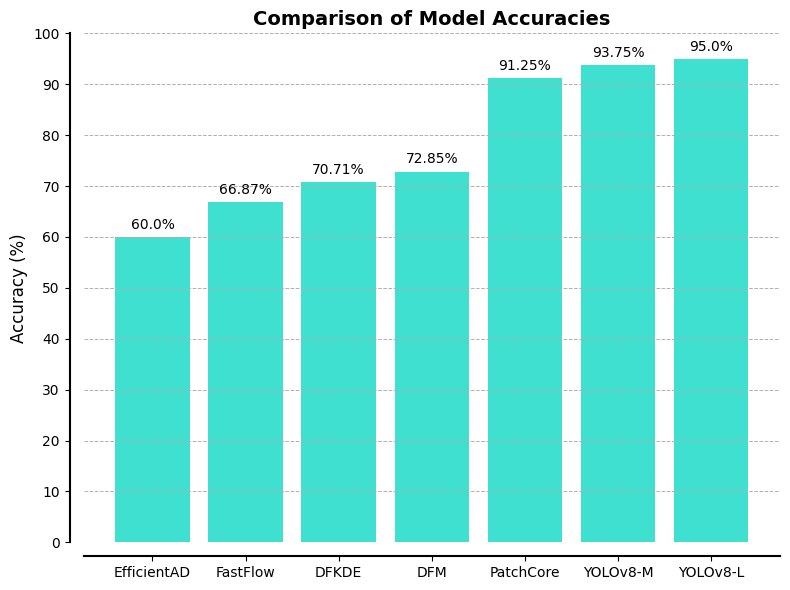
\includegraphics[width=1.1\linewidth]{Rohit_Master_Thesis//Images/bar_chart_model_acc.png}
    \caption{Bar chart representation of the different models accuracy like \gls{yolo}(baseline), our approach including PatchCore, \gls{dfm}, \gls{dfkde}, FastFlow, and EfficientAD.}
    \label{fig:bar chart models accruacy}
\end{figure}

\section{Model-wise breakdown of results}

\subsection*{PatchCore}

\begin{figure}[H]
    \centering
    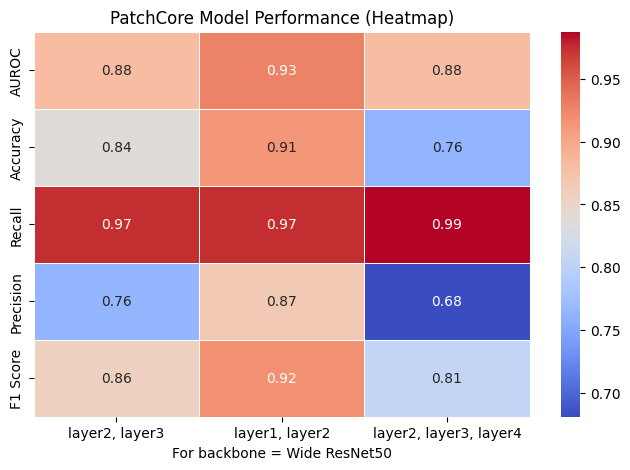
\includegraphics[width=1\linewidth]{Rohit_Master_Thesis//Images/patchcore heatmap.png}
    \caption{PatchCore heatmap for the experiment where backbone "Wide Resnet50" and different layers were used.}
    \label{fig:patchcore heatmap}
\end{figure}

\iffalse
\begin{figure}[ht!]
    \centering  
    % First image
    \begin{minipage}{0.6\textwidth}
        \centering
        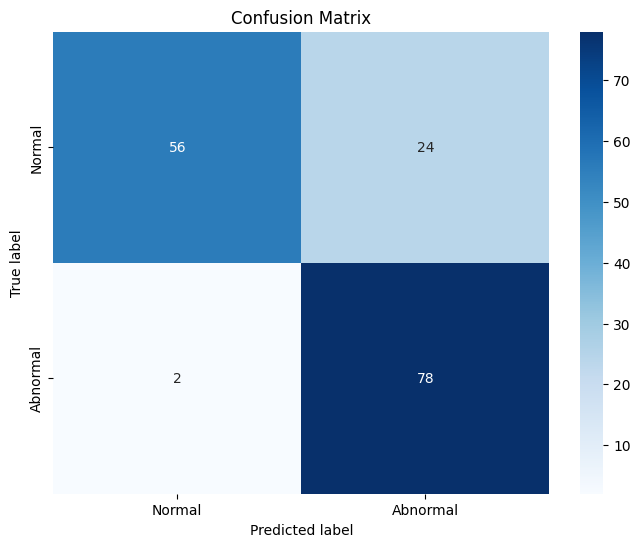
\includegraphics[width=\textwidth]{Rohit_Master_Thesis//Images/patchcore_config1_confusion_matrix.jpg} % Add your image file name here
        \caption{Configuration 1}
    \end{minipage}
    
    \vspace{0.5cm} % Adds vertical space between images
    
    % Second image
    \begin{minipage}{0.6\textwidth}
        \centering
        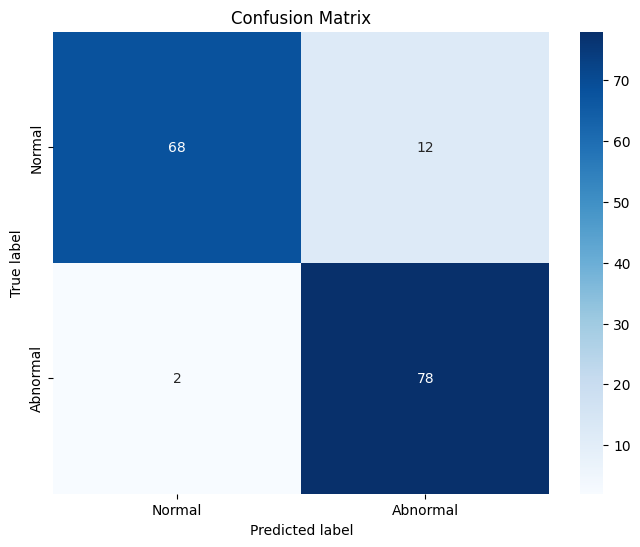
\includegraphics[width=\textwidth]{Rohit_Master_Thesis//Images/patchcore_config2_confusion_matrix.jpg} % Add your image file name here
        \caption{Configuration 2}
    \end{minipage}
    
    \vspace{0.5cm} % Adds vertical space between images
    
    % Third image
    \begin{minipage}{0.6\textwidth}
        \centering
        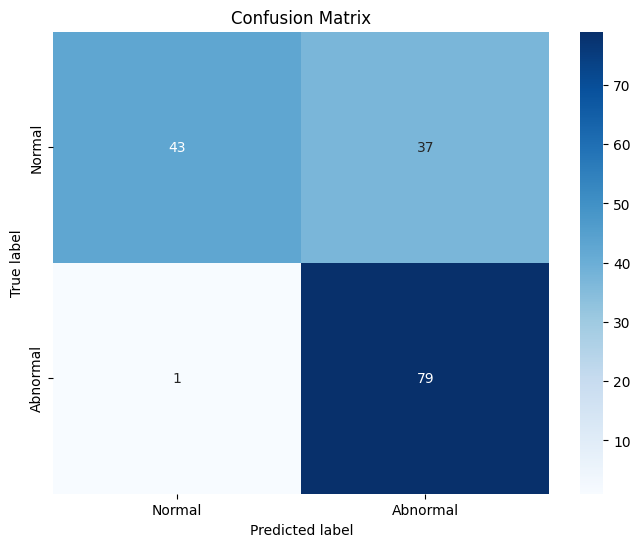
\includegraphics[width=\textwidth]{Rohit_Master_Thesis//Images/patchcore_config3_confusion_matrix.jpg} % Add your image file name here
        \caption{Configuration 3}
    \end{minipage}
    
    \caption{Comparison of Confusion Matrices for Different Configurations.}
    \label{fig:dataset-NG}
\end{figure}
\fi

For this experiment, we employed PatchCore with \texttt{wide\_resnet50\_2} backbone as feature extraction for performing anomaly detection. Firstly, the model extracts feature representations from specific layers of the backbone and then compares the patch-level features of test images with those stored in a memory bank built from normal data. PatchCore uses \gls{k-nn} retrieval for detecting deviations from nominal behavior by calculating the anomaly score based on the distance between patches from the test image and their closest counterparts in the memory bank. This allows PatchCore to perform well when the labeled data is not abundantly available. This model is explained in more detail in \ref{subsec:patchcore}.

For the first configuration, we have used backbone \texttt{wide\_resnet50\_2} with layer2 and layer3 as shown in the heatmap \ref{fig:patchcore heatmap}. This configuration achieves an \gls{auroc} score of 0.8816 and an overall accuracy of 83.75\%. The F1-score was relatively strong at 0.8571, suggesting that the model maintained a balance between precision and recall. The model had a precision of 0.7647, suggesting that sometimes the model classified normal data as anomalous, which resulted in moderate occurrence of false positives, as can be confirmed by the confusion matrix \ref{fig:patchcore config1 confusion matrix}. Whereas the high recall value of 0.975 indicates that the model was highly accurate in detecting almost all the anomalies as anomalies, with some false negatives, as can be seen in the figure \ref{fig:patchcore config1 confusion matrix}.

\begin{figure}[ht!]
    \centering
    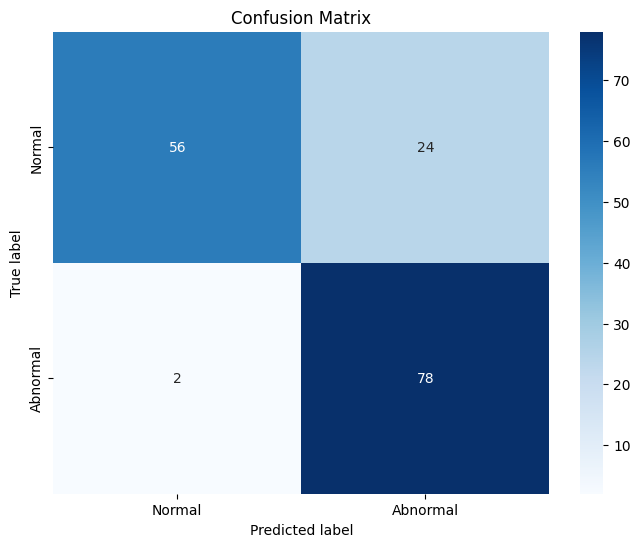
\includegraphics[width=1\linewidth]{Rohit_Master_Thesis//Images/patchcore_config1_confusion_matrix.jpg}
    \caption{Confusion matrix for the first configuration where backbone "Wide Resnet50" and layers "2, 3" were used.}
    \label{fig:patchcore config1 confusion matrix}
\end{figure}

The second configuration resulted in the best overall performance across all metrics, where the feature extraction was carried out by layer1 and layer2 of the same backbone \texttt{wide\_resnet50\_2}. This configuration resulted in a high \gls{auroc} score of 0.9271, with a significant increase in accuracy of 91.25\% as shown in the heatmap \ref{fig:patchcore heatmap}. We also saw improvement in F1-score by about 6.6\% from the previous configuration, reaching 0.9176, indicating an even better balance between precision and recall. The precision improved to 0.8667, indicating a reduction in false positives as seen in the confusion matrix \ref{fig:patchcore config2 confusion matrix} where the false positives were reduced by 50\% from the first configuration. While the recall remained high but the same as the first configuration at 0.975, meaning the model continued to detect almost all anomalies, as shown in the figure \ref{fig:patchcore config2 confusion matrix}. The improved performance of this configuration can be due to the use of features from the combination of layer 1 and layer 2, which incorporates the combination of both low-level and mid-level features. Low-level features might allow the model to detect fine-grained details, while layer 2 might provide the more complex structures needed to detect anomalies. These features can provide a richer, more detailed representation of normal data, making the detection of anomalies without overfitting normal data easier.

\begin{figure}[ht!]
    \centering
    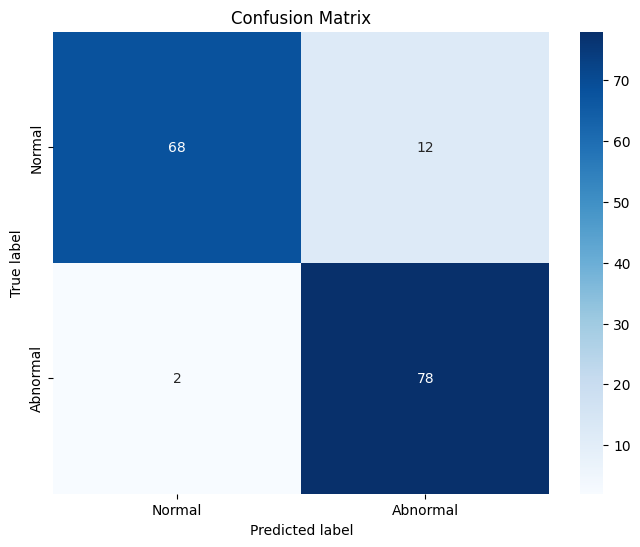
\includegraphics[width=1\linewidth]{Rohit_Master_Thesis//Images/patchcore_config2_confusion_matrix.jpg}
    \caption{Confusion matrix for the second configuration where backbone "Wide Resnet50" and layers "1, 2" were used.}
    \label{fig:patchcore config2 confusion matrix}
\end{figure}

In the third configuration, layer 2, layer 3, and layer 4 were used for the backbone \texttt{wide\_resnet50\_2}, it resulted in a lower \gls{auroc}score of 0.8807 which is almost equal to the \gls{auroc} score for first configuration, and the accuracy we got is 76.25\% which is the lowest of all the configuration. The F1-score also decreased slightly to 0.8061 due to a drop in precision value to 0.6810. This lower precision indicates that the model produced a higher number of false positives, i.e., more normal images were classified as anomalous, as can be seen in confusion matrix \ref{fig:patchcore config3 confusion matrix} where out of 80 normal images, 37 were classified as anomalous. However, the recall was the highest at 0.9875, which means that the model was still able to detect almost all of the anomalies, as seen in the figure \ref{fig:patchcore config3 confusion matrix} out of 80, 79 were correctly classified as anomalous with only one being misclassified as normal. The inclusion of deeper layers, like layer 4, probably introduced more abstract features, which may have been less effective for the detection of fine-grained anomalies, resulting in the reduction of overall performance. This configuration highlights the importance of extraction of features from appropriate layers for ensuring balance between detecting true anomalies and avoiding excessive false positives.

\begin{figure}[ht!]
    \centering
    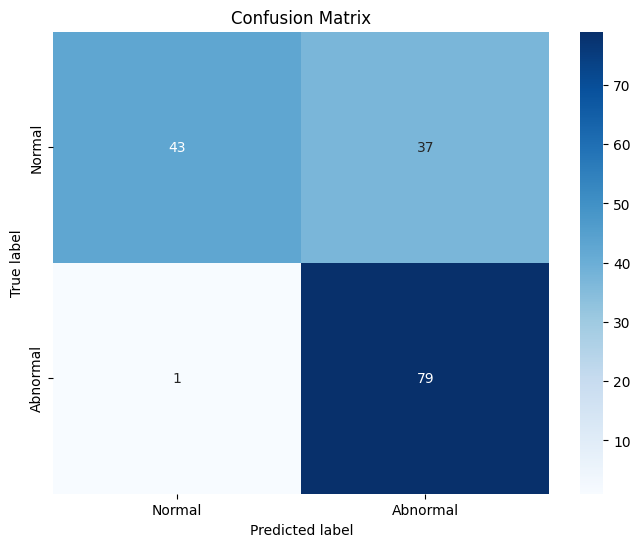
\includegraphics[width=1\linewidth]{Rohit_Master_Thesis//Images/patchcore_config3_confusion_matrix.jpg}
    \caption{Confusion matrix for the third configuration where backbone "Wide Resnet50" and layers "2, 3, 4" were used.}
    \label{fig:patchcore config3 confusion matrix}
\end{figure}

Now let's look at how the best performing configuration of PatchCore image classification results. When performing image classification, three images are generated one is the original image which we provided to perform classification on, then the predicted heat map generated by the model is shown, and finally the predicted label for the image and its score is given, as shown in the figure \ref{fig:IC-results-patchcore}. When the image is predicted as normal, then no heat map is generated.

\begin{figure}[ht!]
    \centering  
    \begin{minipage}{1\textwidth}
        \centering
        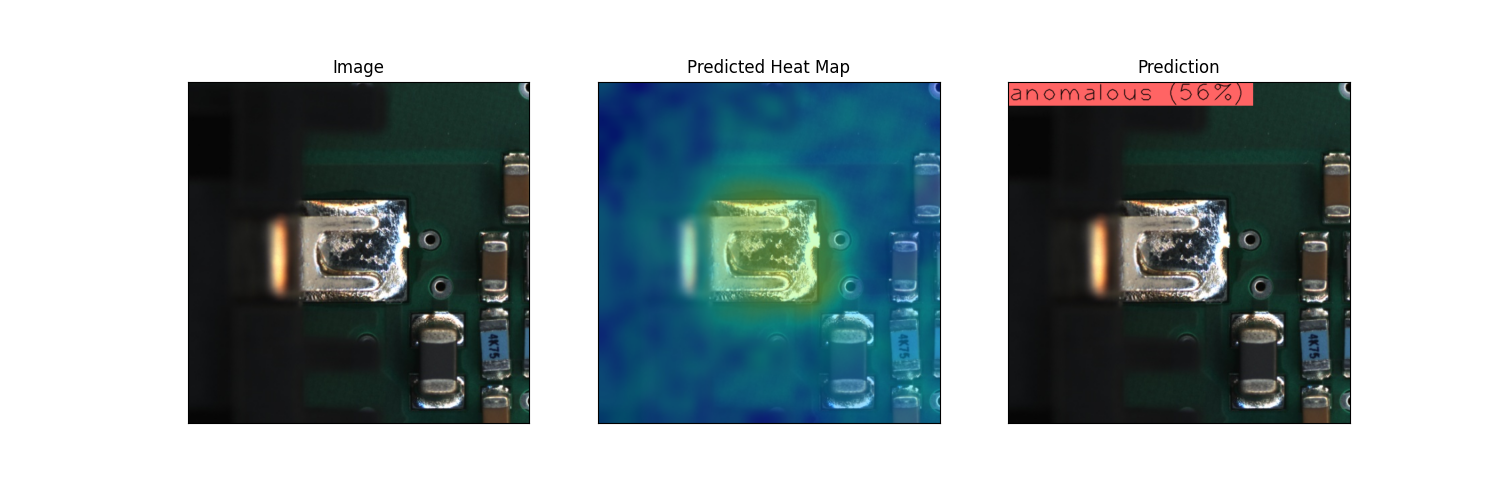
\includegraphics[width=1\textwidth]{Rohit_Master_Thesis//Images/IC_NG.png} % Add your image file name here
        %\caption{Caption for the first image.}
    \end{minipage}
    
    %\vspace{5pt} % Adjust the space between images

    \begin{minipage}{1\textwidth}
        \centering
        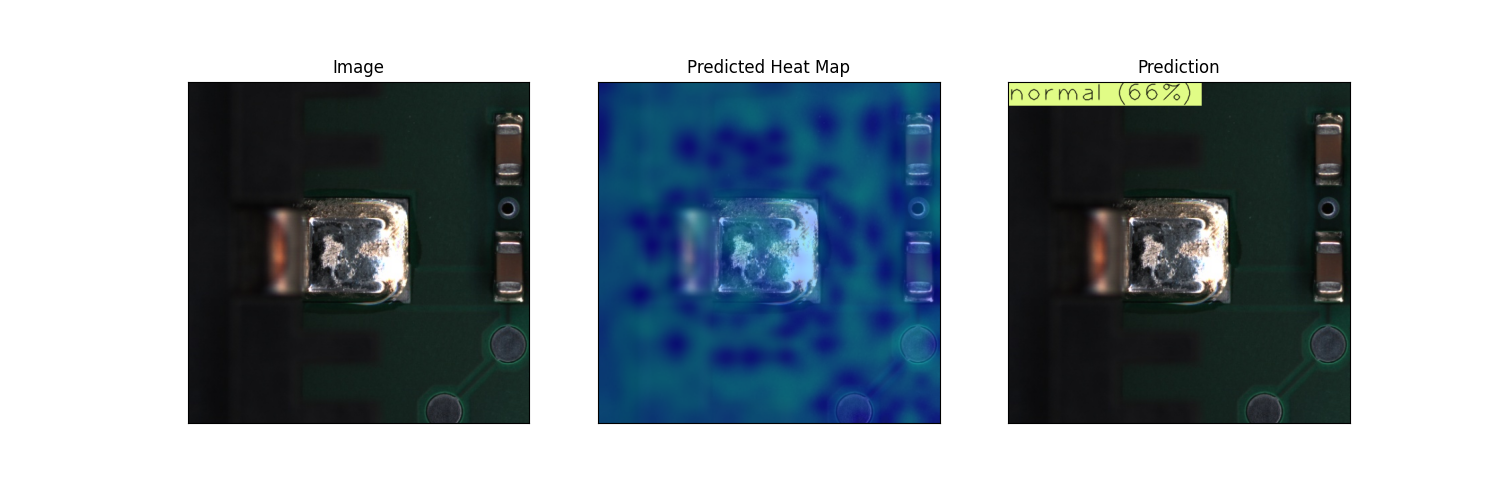
\includegraphics[width=1\textwidth]{Rohit_Master_Thesis//Images/IC_FC.png} % Add your image file name here
        %\caption{Caption for the second image.}
    \end{minipage}
    
    %\vspace{10pt} % Adjust the space between images

    \begin{minipage}{1\textwidth}
        \centering
        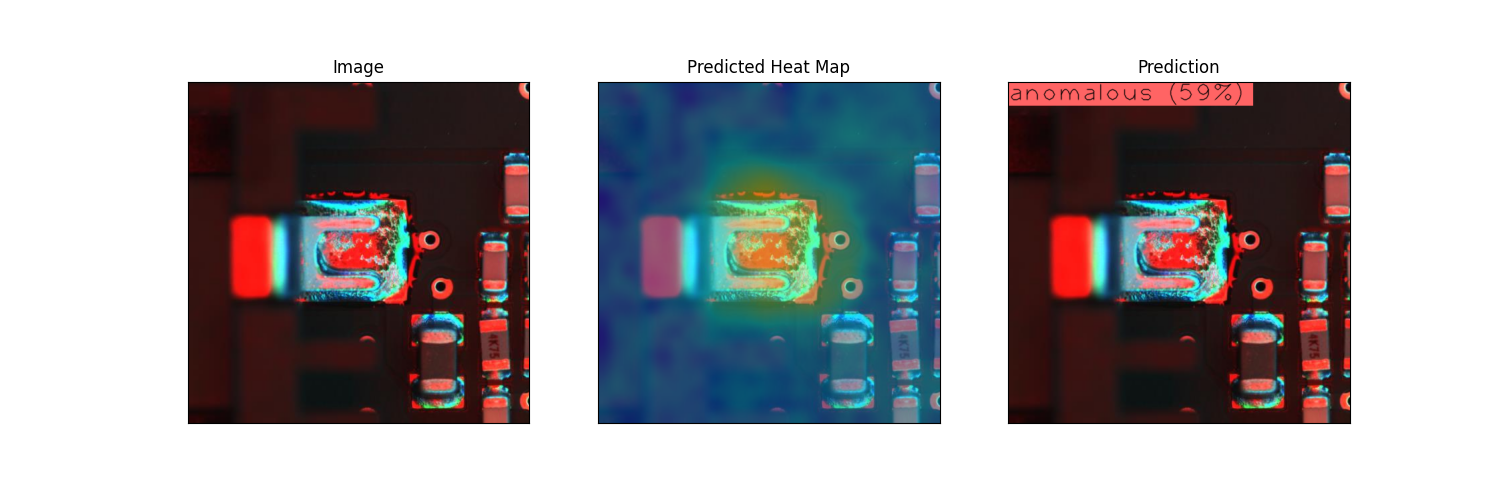
\includegraphics[width=1\textwidth]{Rohit_Master_Thesis//Images/IC_NG2.png} % Add your image file name here
        %\caption{Caption for the third image.}
    \end{minipage}
    
    \caption{Results of image classification using second configuration(best performing) for PatchCore model.}
    \label{fig:IC-results-patchcore}
\end{figure}

Lastly, we also performed Image Segmentation using the best performing configuration of PatchCore model, an example of its results can be seen in the figure \ref{fig:IS-results-patchcore}. For the image segmentation, four images are generated in total. The first two are similar to the image classification results, but as the task here is segmentation, when the image is predicted as anomalous, it also generates a predicted mask of where the anomaly is, as shown in the last image of the top of the figure \ref{fig:IS-results-patchcore} marked with a red line. And when there is no anomaly detected it is just blank.

\begin{figure}[ht!]
    \centering  
    \begin{minipage}{1\textwidth}
        \centering
        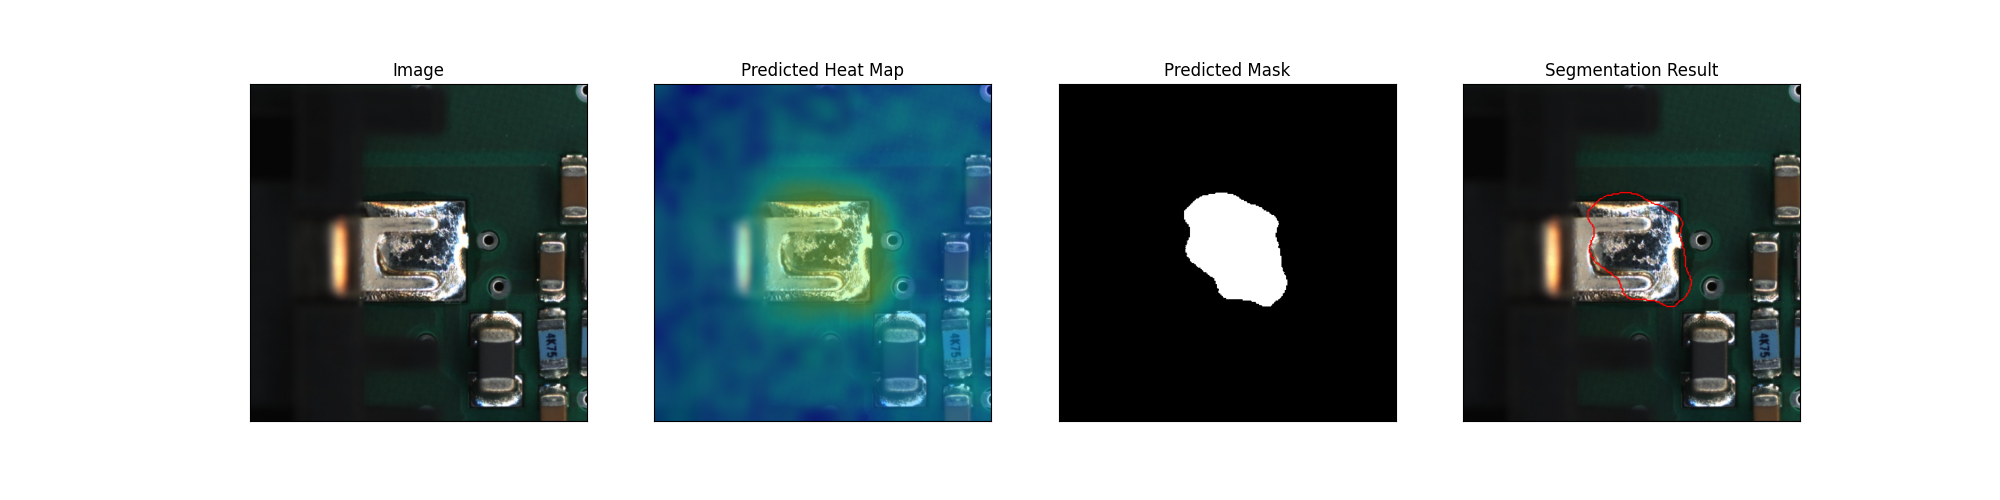
\includegraphics[width=1\textwidth]{Rohit_Master_Thesis//Images/IS_NG1.png} % Add your image file name here
        %\caption{Caption for the first image.}
    \end{minipage}
    
    %\vspace{5pt} % Adjust the space between images

    \begin{minipage}{1\textwidth}
        \centering
        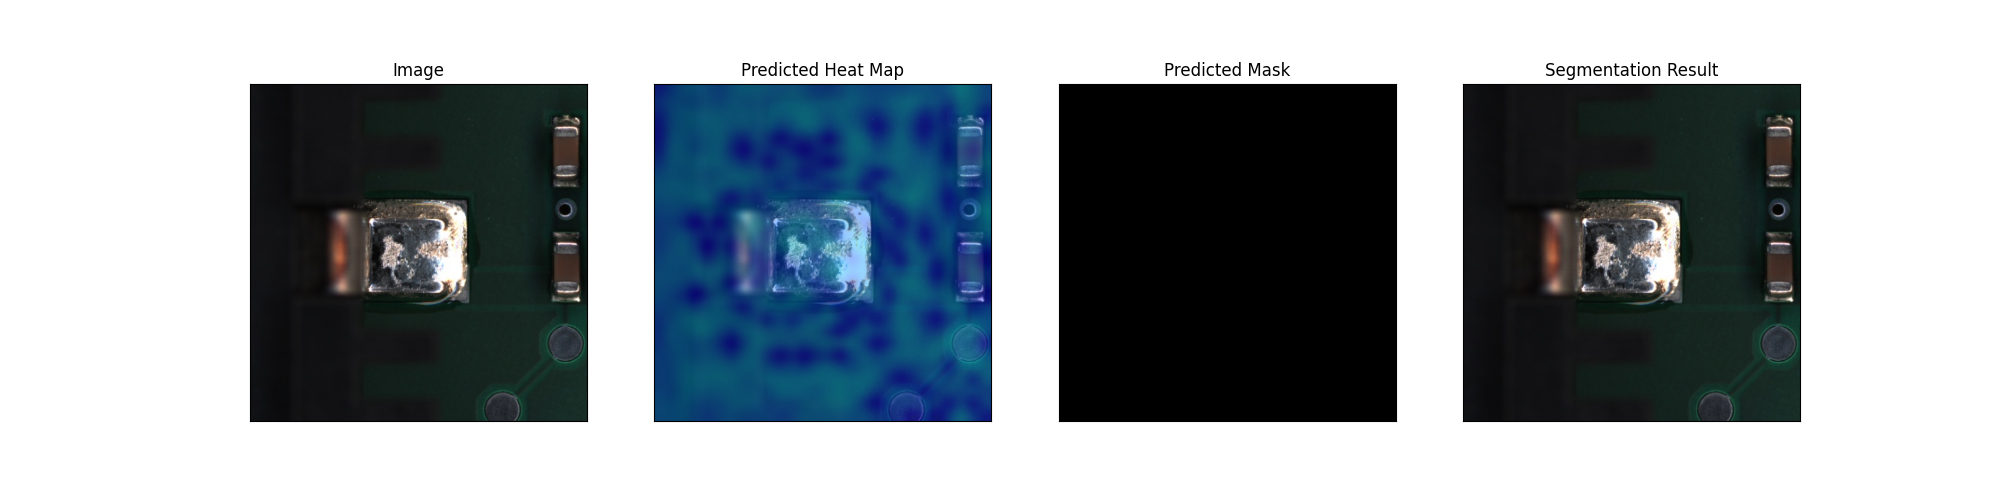
\includegraphics[width=1\textwidth]{Rohit_Master_Thesis//Images/IS_FC.png} % Add your image file name here
        %\caption{Caption for the second image.}
    \end{minipage}
    
    \caption{Results of image segmentation using second configuration(best performing) for PatchCore model.}
    \label{fig:IS-results-patchcore}
\end{figure}

Both the image classification and segmentation results, helps us visualize how the model is performing in real world where we can see what is the predicted label and the anomaly score given for that image, with that also if the image is anomalous, with the help of the model we can pinpoint where the anomaly must be.

\subsection*{\gls{yolo}}

Two different model sizes of \gls{yolo}v8 \cite{Ultralytics2024} were evaluated for this experiment: \gls{yolo}v8-M(medium) and \gls{yolo}v8-L(large). Both the models were trained for 200 epochs on the training dataset.

The \textbf{\gls{yolo}v8-L} model, which is larger and more complex, reached an accuracy of 95\% after 200 epochs. The model's high accuracy could be due to its increase in the depth and number of parameters, which allows it to capture more detailed and complex patterns in the dataset. Also it being a supervised model, having access to all the labels while training helps it to learn better and fit the model well to the data.

\begin{figure}[ht!]
    \centering
    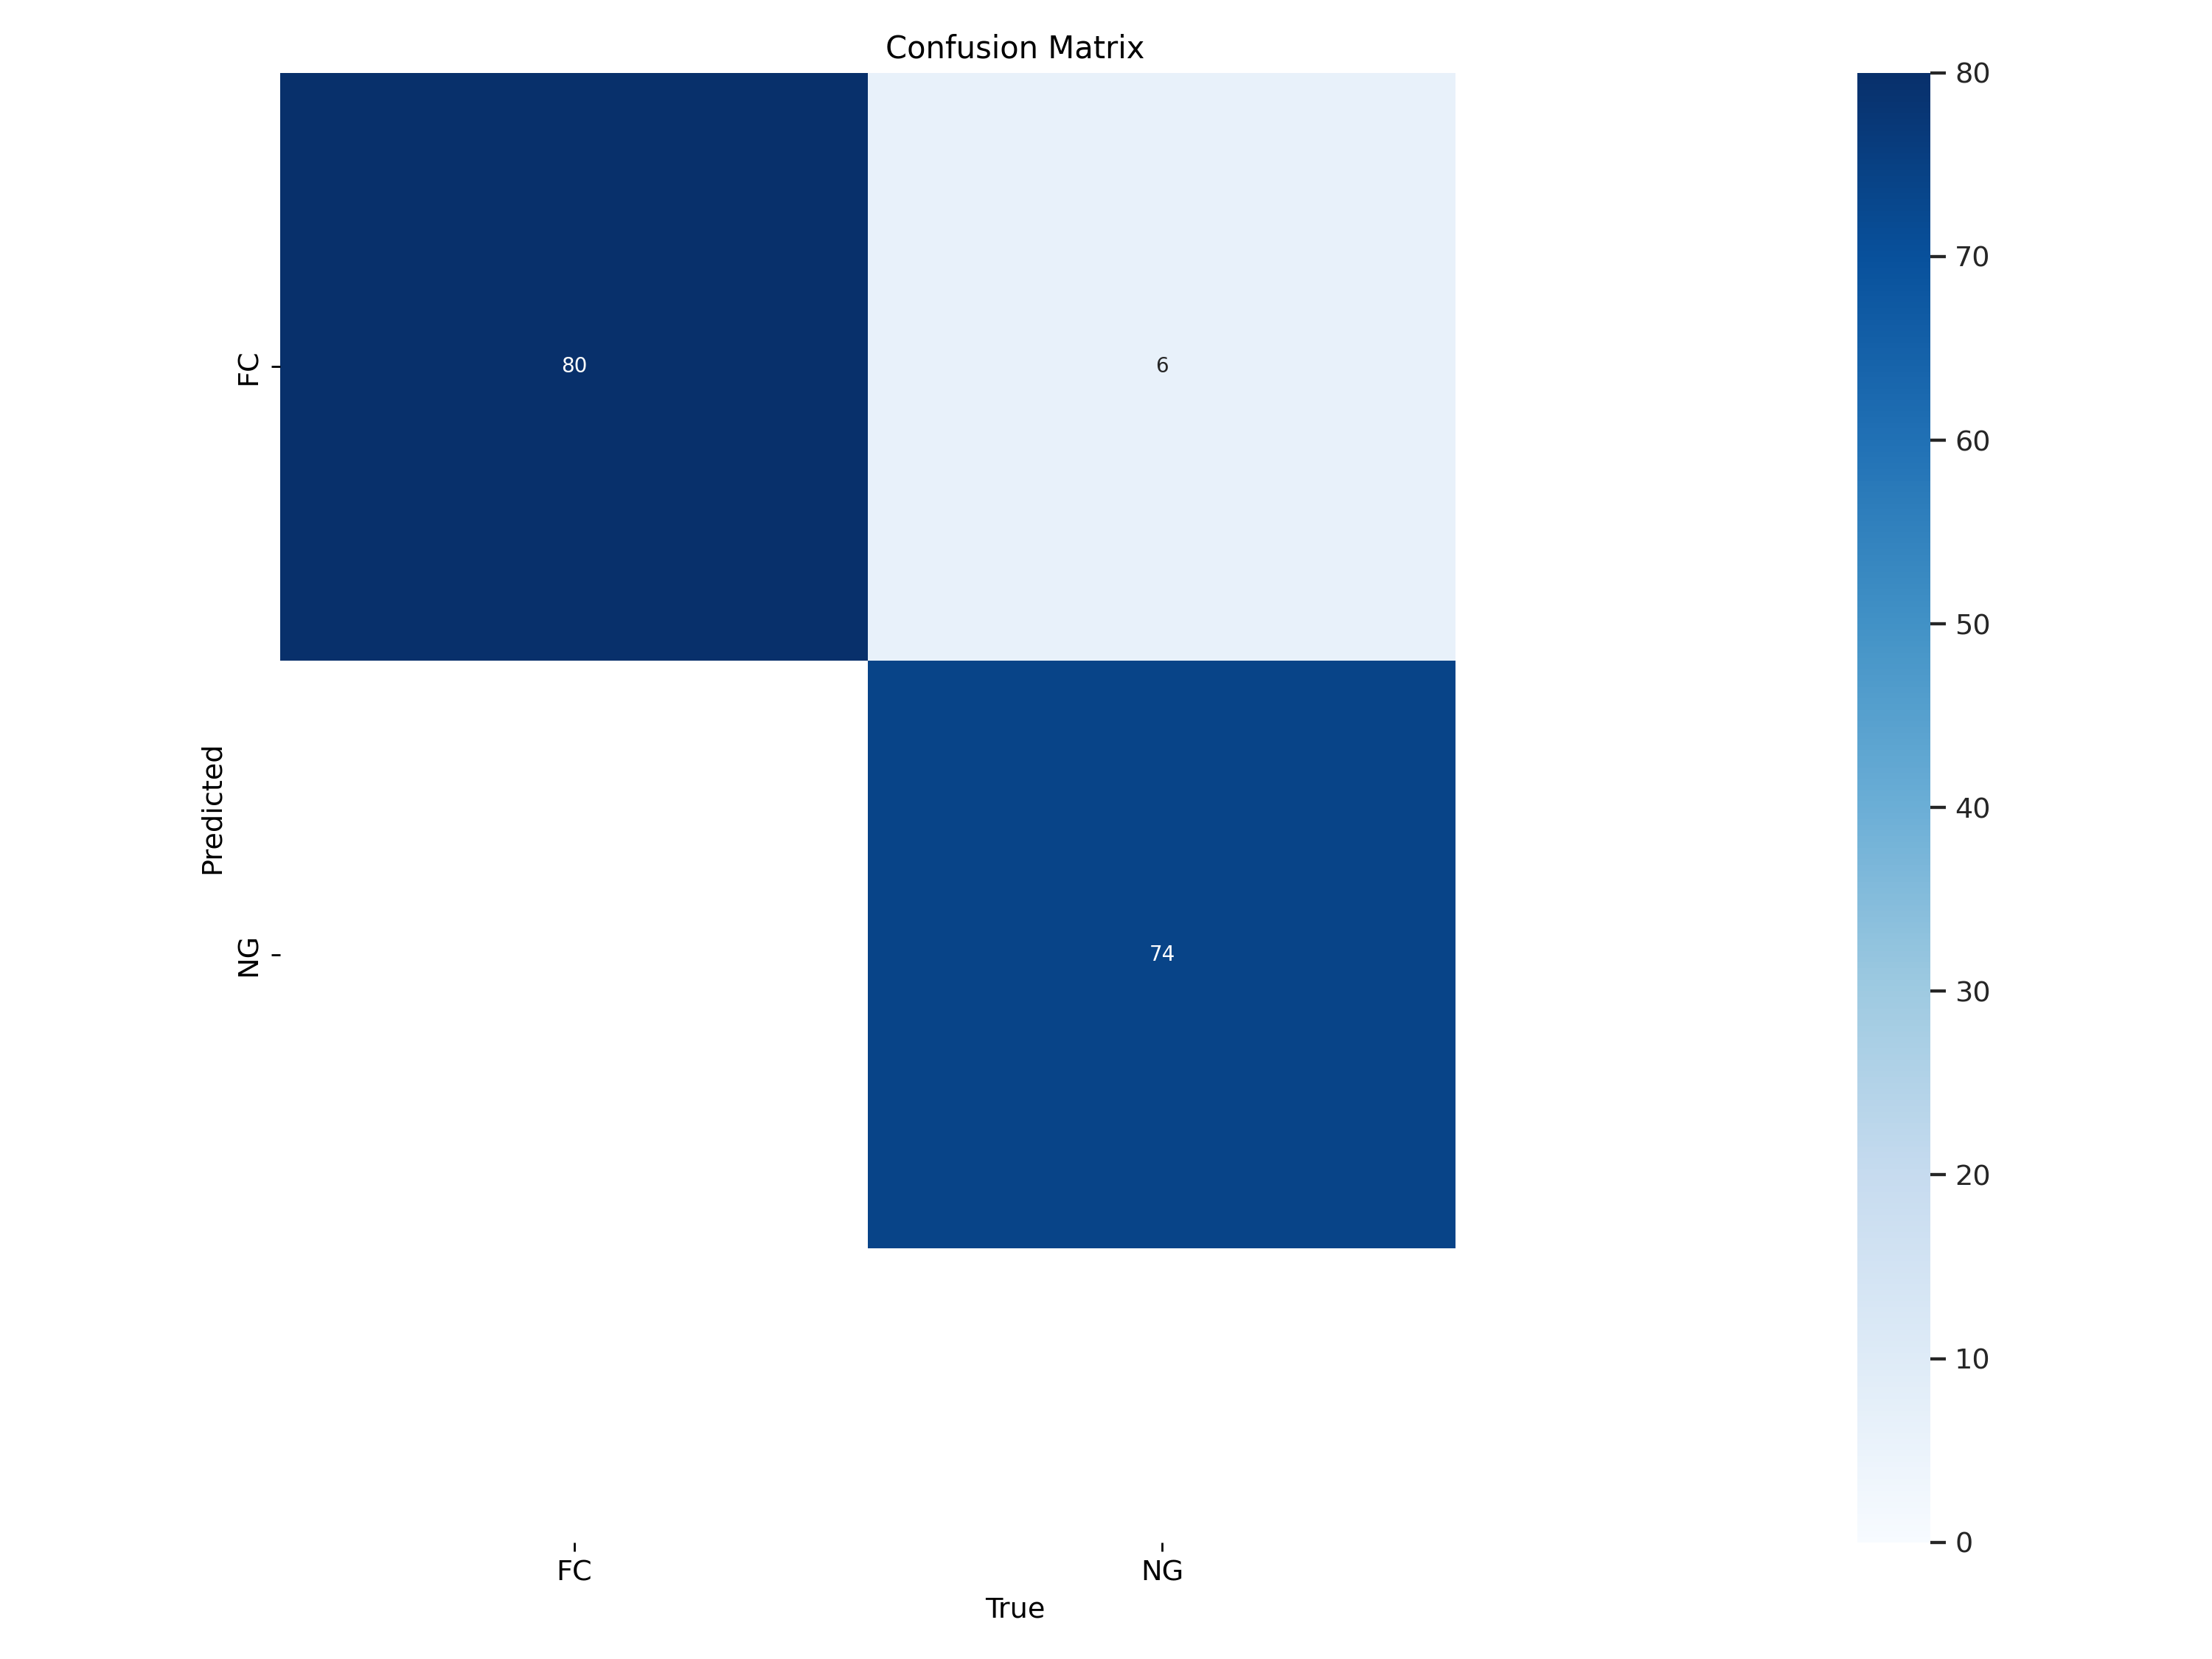
\includegraphics[width=1.3\linewidth]{Rohit_Master_Thesis//Images/yolov8l_confusion_matrix.png}
    \caption{Confusion matrix for the baseline model \gls{yolo}v8-L, its accuracy is 95\%}
    \label{fig:yolov8l confusion matrix}
\end{figure}

The confusion matrix, as shown in figure \ref{fig:yolov8l confusion matrix}, provides a more detailed look into how well the model performs in the classification task. We can see that the model was able to correctly classify all the normal(FC) images as normal. While only 6 were false positives, i.e., anomalous(NG) images were classified as normal images, the rest of the 74 were correctly classified as NG, i.e., True Negatives. These values are consistent with the precision, recall, and F1-score results as shown in table \ref{tab:yolov8_performance}. The precision of 1.0 highlights the model's reliability in predicting normal(FC) instances, as it did not make any incorrect predictions for that class. The recall of 0.925, while still quite good, indicates that the model misclassified a small number of anomalous(NG) as normal(FC). With the impressive F1-score of 0.9615, shows the models well-rounded performance.

\begin{table}[ht!]
    \centering
    \begin{tabular}{|c|c|c|c|c|}
        \hline
        \textbf{Model} & \textbf{Accuracy} & \textbf{Precision} & \textbf{Recall} & \textbf{F1-score} \\ \hline
        \textbf{YOLOv8-M} & 93.75\% & 0.9867 & 0.925 & 0.9547 \\ \hline
        \textbf{YOLOv8-L} & 95\% & 1.0 & 0.925 & 0.9615 \\ \hline
    \end{tabular}
    \caption{Comparison of YOLOv8-M and YOLOv8-L Model Performance}
    \label{tab:yolov8_performance}
\end{table}

%Probably for discussion section(remember to paraphrase)
%Explanation of Results
%The performance of YOLOv8-L is in line with its design as a larger, more powerful model. The depth and complexity of the YOLOv8-L architecture allow it to capture a wide variety of patterns and features in the data, leading to its high precision and recall. The non-maximum suppression (NMS) technique used in YOLOv8 helps further refine the predictions by ensuring that overlapping bounding boxes are filtered, resulting in more accurate object classification. Additionally, YOLOv8-L's anchor-free detection mechanism improves its ability to generalize across objects of various sizes, contributing to its robustness in detecting NG and FC items.

The \textbf{\gls{yolo}v8-M} model, which is smaller and more lightweight when compared to \gls{yolo}v8-L, reaches an accuracy of 93.75\%. This is slightly lower than its bigger model, as seen from the table \ref{tab:yolov8_performance}, but its overall performance was still quite impressive.

\begin{figure}[ht!]
    \centering
    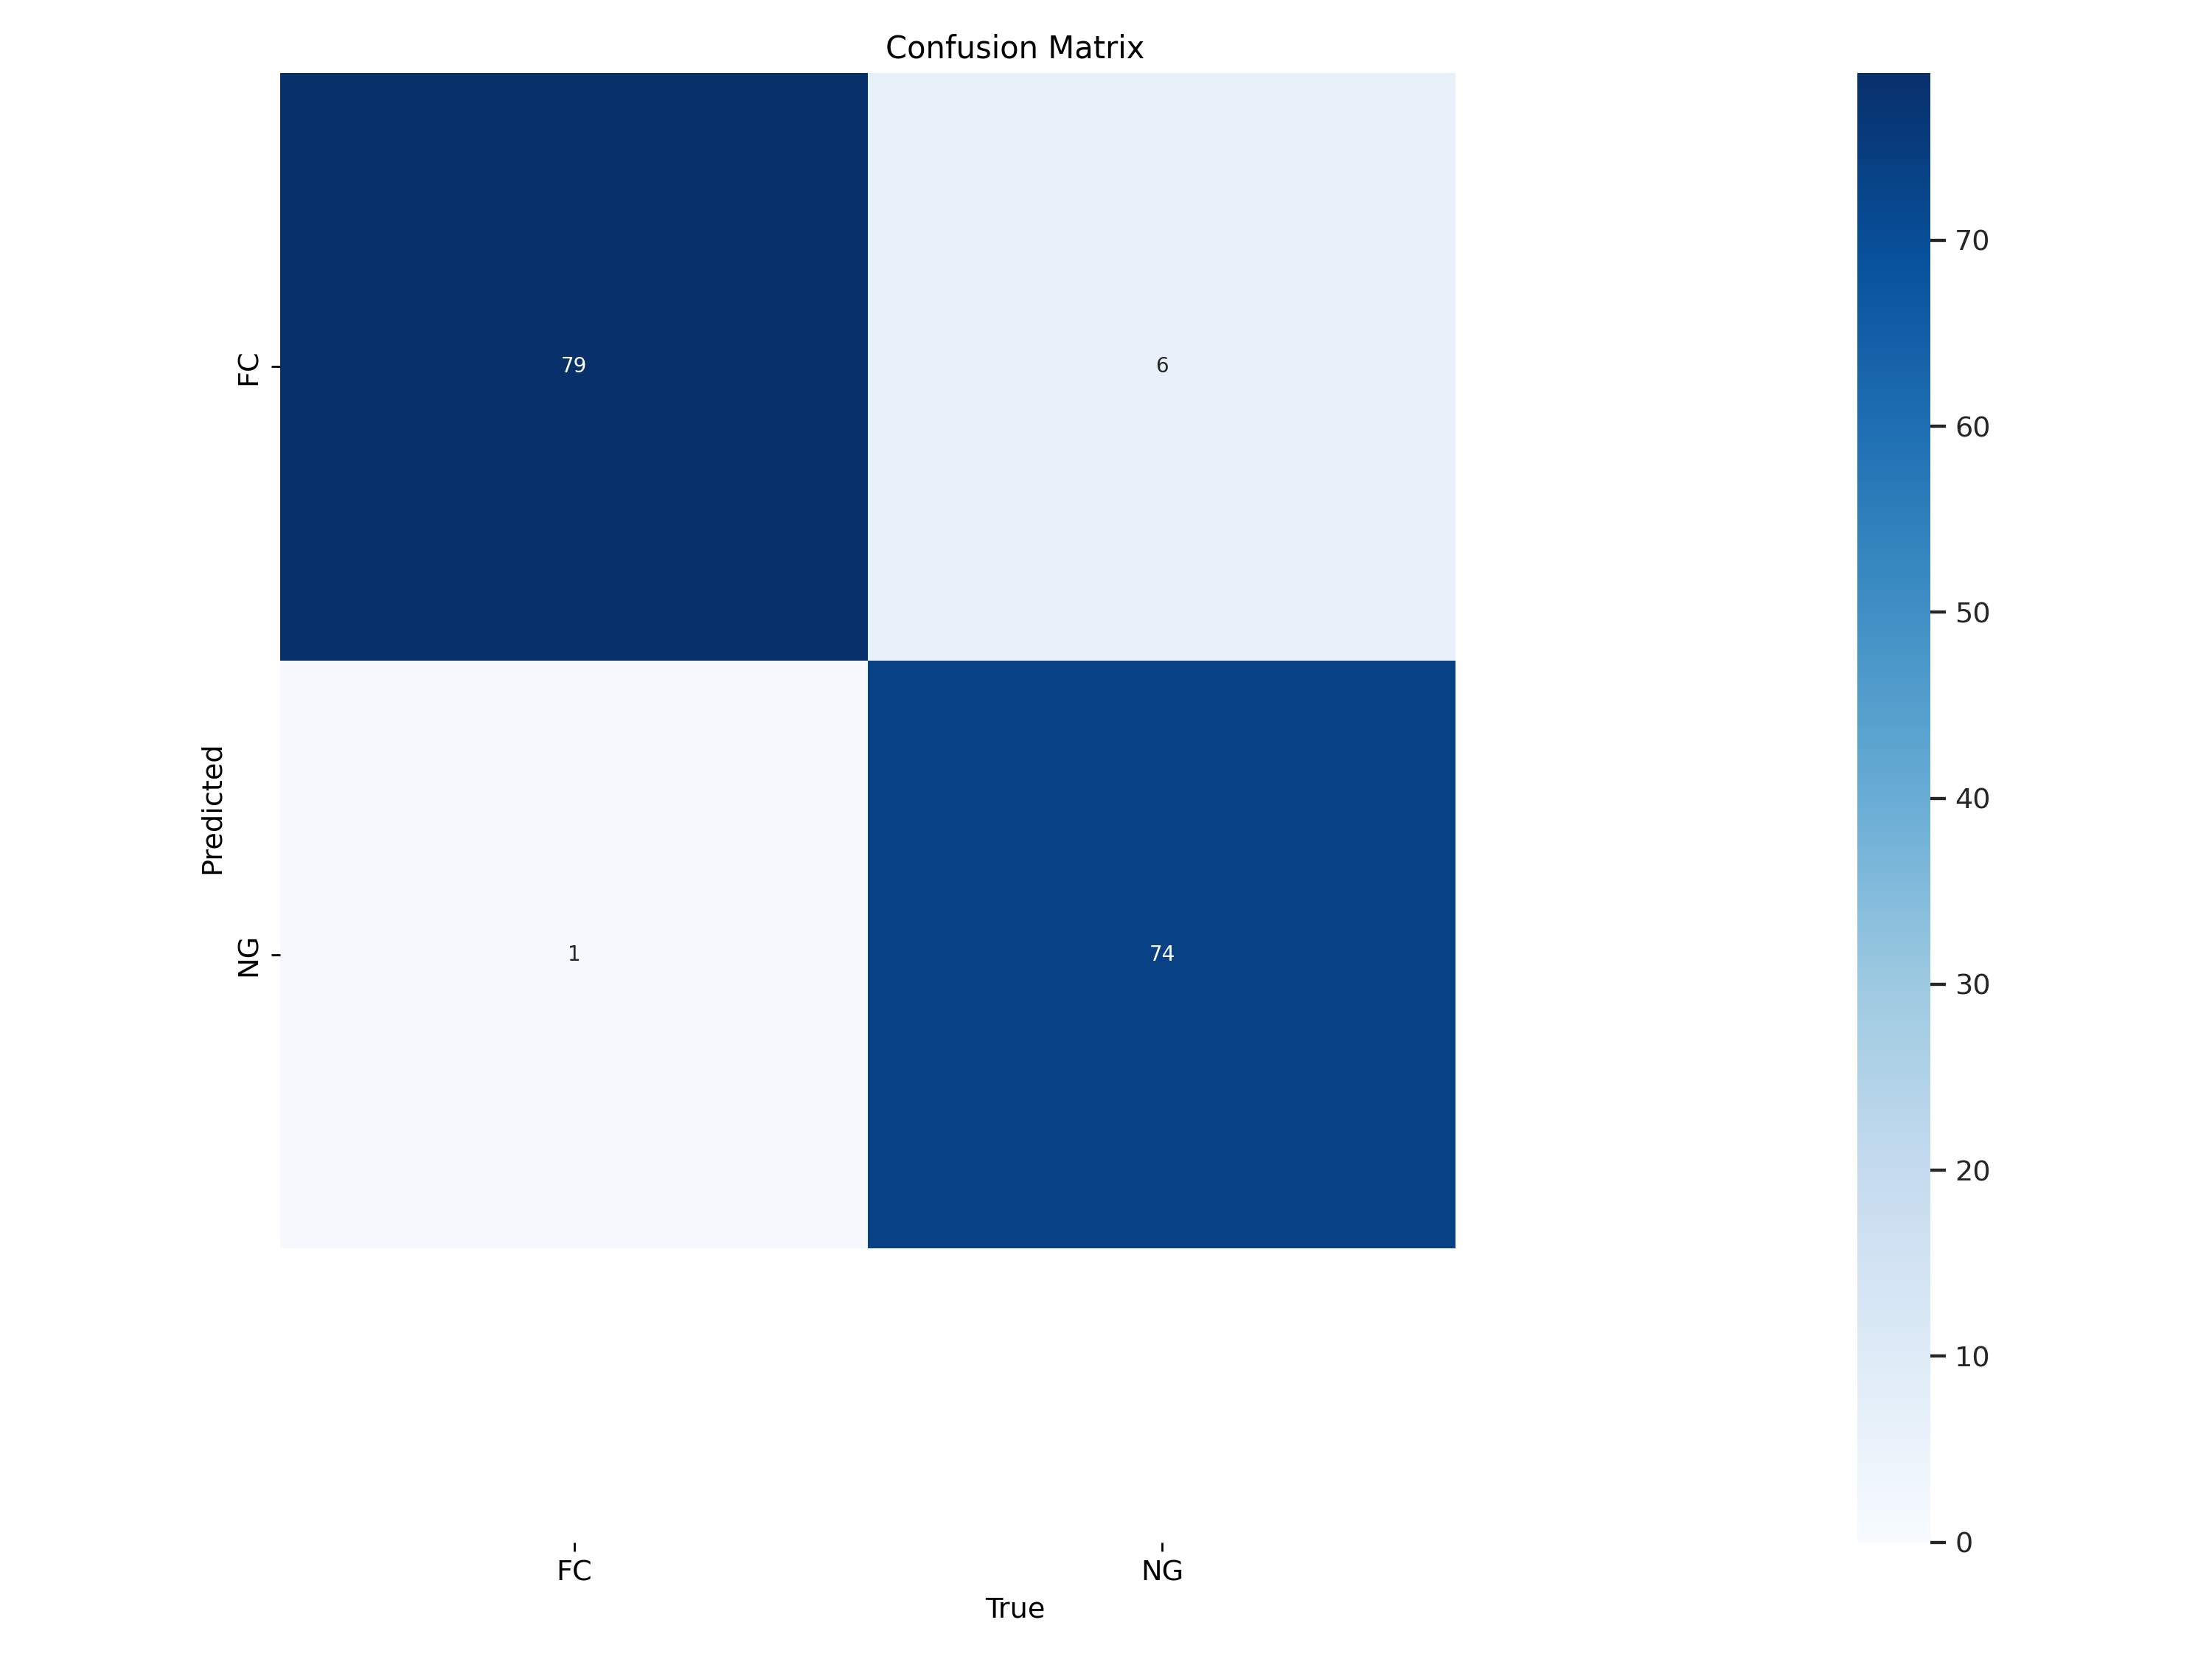
\includegraphics[width=1.3\linewidth]{Rohit_Master_Thesis//Images/yolov8m_confusion_matrix.png}
    \caption{Confusion matrix for the baseline model \gls{yolo}v8-M, its accuracy is 93.75\%}
    \label{fig:yolov8m confusion matrix}
\end{figure}

The confusion matrix in figure \ref{fig:yolov8m confusion matrix} shows almost similar results to that of \gls{yolo}v8-L. With 79 True positives and 74 true negatives, while only making 6 false positives and 1 false negative prediction, apart from the 1 misclassified normal image as anomalous, the results are similar to that of \gls{yolo}v8-L. This indicates that the performance of the \gls{yolo}v8-M, though highly accurate, still falls just short of \gls{yolo}v8-L's performance due to its smaller capacity for learning complex patterns. As can be seen from the table \ref{tab:yolov8_performance}, the model achieved a precision of 0.9867, meaning that almost all of the predictions of normal(FC) images were correct. The recall for both the \gls{yolo}v8-L and \gls{yolo}v8-M matches and is equal to 0.925, indicating that both models successfully detected the same number of FC cases. The F1-score of the model was 0.9547, which is slightly lower than \gls{yolo}v8-L due to the slight decrease in the precision. While the model was highly accurate, it did produce a small number of false positives, in this case, 6 anomalous(NG) images were misclassified as normal(FC), which reduced its precision slightly.

%See if you need to include loss and accuracy curve for both the models of YOLO

%Probably for discussion section(remember to paraphrase)
%Explanation of Results

%YOLOv8-M strikes a balance between computational efficiency and accuracy. The model achieves 93.75\% accuracy, which is competitive given its smaller architecture compared to YOLOv8-L. The slightly lower performance is expected due to YOLOv8-M’s reduced depth and number of parameters, which limits its ability to capture as many intricate patterns in the data as YOLOv8-L. However, YOLOv8-M’s simpler structure makes it faster and more computationally efficient, making it suitable for tasks where real-time performance and resource limitations are important.

%Model Comparison and Insights
%YOLOv8-L outperforms YOLOv8-M by achieving 95\% accuracy, compared to YOLOv8-M’s 93.75\%. This difference in performance can be attributed to the larger number of layers and parameters in YOLOv8-L, which allows it to capture more detailed features from the dataset. YOLOv8-L’s larger architecture is particularly beneficial for classification tasks that involve complex patterns or subtle differences between classes, making it a better choice for applications where accuracy is critical.

%However, YOLOv8-M offers significant advantages in terms of speed and computational efficiency. Despite having fewer layers, YOLOv8-M achieves strong results, making it a good option for scenarios where real-time inference is necessary or where computational resources are limited. The slight trade-off in accuracy is reasonable given the gains in efficiency, making YOLOv8-M ideal for environments where fast processing is prioritized over achieving the highest possible accuracy.

\subsection*{\gls{dfm}}

In this section, we will look into the results obtained from various experiments using \gls{dfm}. \gls{dfm} is explained in the section \ref{subsec:dfm}, and in our experiments, we evaluated \gls{dfm} performance using various backbones, their layers, and pooling techniques to explore the robustness and accuracy of the model. Below the results are divided based on the backbone used. 

\subsubsection*{ResNet50}

Here, we used ResNet50's layer4 for feature extraction along with \gls{nll} as the scoring type. This gave us the \gls{auroc} score of 0.6309 and F1-score of 0.6689, with an overall accuracy of 50.7\%, which is not very good, as can be seen from the table \ref{tab:dfm resnet results}, it is basically doing random guessing. The low F1-score suggests that while the model was good at detecting anomalies, it struggled with precision because of the high number of false positives. These findings suggest that using features extracted from higher layers, like layer 4, may have led the model to focus on more abstract, high-level features that are less effective at determining anomalies from normal samples.

\begin{table}[ht!]
    \centering
    \begin{tabular}{|l|c|c|c|c|c|}
        \hline
        \textbf{Model} & \textbf{Accuracy (\%)} & \textbf{\gls{auroc}} &\textbf{Precision} & \textbf{Recall} & \textbf{F1-score} \\ \hline
        ResNet50 & 50.71\% & 0.6309 & 0.5036 & 1.0 & 0.6699 \\ \hline
        Wide-ResNet50-2 (layer2, nll) & 60\% & 0.6382 & 0.5556 & 1.0 & 0.7143 \\ \hline
        Wide-ResNet50-2 (layer2, fre) & 62.12\% & 0.5795 & 0.5681 & 1.0 & 0.7254 \\ \hline
        Wide-ResNet50-2 (layer3) & 62.86\% & 0.7265 & 0.5738 & 1.0 & 0.7292 \\ \hline
    \end{tabular}
    \caption{Results for ResNet and Wide-ResNet50-2 Backbones}
    \label{tab:dfm resnet results}
\end{table}

Another configuration that we tried was using a different variant of ResNet50 called Wide-ResNet50-2 and performing feature extraction using layer 2 while keeping the \gls{pca} level at 0.97 and using \gls{nll} score type. This resulted in a slight improvement in both the accuracy and \gls{auroc} score of 60\% and 0.6382, respectively. The precision improved to 0.5556, while the recall stayed at 1.0, resulting in an F1-score of 0.7143, as shown in the table \ref{tab:dfm resnet results}. Along with that, we also performed a similar experiment by keeping the backbone and layer the same but changing the \gls{pca} level to 0.995 and scoring type to \gls{fre}. This resulted in much better compared to when we used scoring type as \gls{nll}, where accuracy increased by about 2\% to 62.12\% while seeing a drop in \gls{auroc} to 0.5795. The recall stayed the same at 1.0, but a slight increase in precision was observed to 0.5681, therefore increasing the F1-score to 0.7254. This improvement in both precision and F1-score shows that lower-level features from layer 2 were more effective at capturing variations between normal and anomalous images. Finally, after seeing better results with \gls{fre} scoring type, we experimented with one more layer of the same backbone. The layer used here was layer 3, and with this, we again saw slight improvement across all the metrics. The accuracy came out to be 62.86\% which is a small incremental update, while with \gls{auroc} score we saw an improvement of about 25\% when compared to Wide-ResNet50-2 (layer2, \gls{fre}) of the table \ref{tab:dfm resnet results}, and saw a rise of about 14\% when compared with Wide-ResNet50-2 (layer2, \gls{nll}). Other layers were also tried for both the ResNet50 and Wide-ResNet50-2 backbone, but all of them resulted in the model just randomly guessing the predictions, i.e., the accuracy was 50\%.

\subsubsection*{Densenet}

Next, we conducted experiments using different DenseNet backbones. Firstly, we used DenseNet121, which extracted features from the features.norm5 layer and the \gls{fre} score type. This configuration improved the model's performance further, with an \gls{auroc} score of 0.7309 and an accuracy of 61.43\%. The model reached a precision of 0.5645 and a recall of 1.0, giving an F1-score of 0.7216. These improved scores suggest that the DenseNet architecture, which relies on dense connections and feature reuse, contributed to improved feature representations for anomaly detection. Table \ref{tab:dfm densenet results} shows the results of different backbones of DenseNet.

\begin{table}[ht!]
    \centering
    \begin{tabular}{|l|c|c|c|c|c|}
        \hline
        \textbf{Model} & \textbf{AUROC} & \textbf{Accuracy} & \textbf{Precision} & \textbf{Recall} & \textbf{F1-score} \\ \hline
        DenseNet121 & 0.7310 & 0.6143 & 0.5645 & 1.0 & 0.7216 \\ \hline
        DenseNet169 (norm5) & 0.7456 & 0.6571 & 0.5932 & 1.0 & 0.7447 \\ \hline
        \textbf{DenseNet169 (denseblock3, 0.97 PCA)} & \textbf{0.7203} & \textbf{0.7286} & 0.6538 & 0.9714 & 0.7816 \\ \hline
        DenseNet169 (denseblock3, 0.995 PCA) & 0.7190 & 0.7214 & 0.6422 & 1.0 & 0.7821 \\ \hline
        DenseNet201 (denseblock3, 0.995 PCA) & 0.7259 & 0.7143 & 0.6389 & 0.9857 & 0.7753 \\ \hline
        %DenseNet264d (untrained) & 0.8029 & N/A & N/A & N/A & 0.8471 \\ \hline
        %DenseNet201 (denseblock3, 0.97 PCA) & 0.7265 & N/A & N/A & N/A & 0.8460 \\ \hline
    \end{tabular}
    \caption{Results for DenseNet Backbones}
    \label{tab:dfm densenet results}
\end{table}

The best performing configuration for the DenseNet architecture comes from the DenseNet169 backbone, with features extracted from features.denseblock3 layer, a \gls{pca} level of 0.97, and the \gls{fre} score type as shown in the table \ref{tab:dfm densenet results}. This configuration gave an \gls{auroc} score of 0.7203 and an accuracy of 72.86\%. Precision also improved to 0.6538. While recall reduced slightly, it remained high at 0.9714, resulting in an F1-score of 0.7816. This improvement in both the precision and the F1-score suggests that the DenseNet169's larger size allowed for better feature extraction and classification, particularly when extracting features from the third dense block. The high recall score indicates that the model was able to detect most of the anomalies, as can be seen in the confusion matrix \ref{fig:dfm densenet169 confusion matrix}, while the increase in precision value indicates a significant reduction in the number of false positives relative to other configurations.

\begin{figure}[ht!]
    \centering
    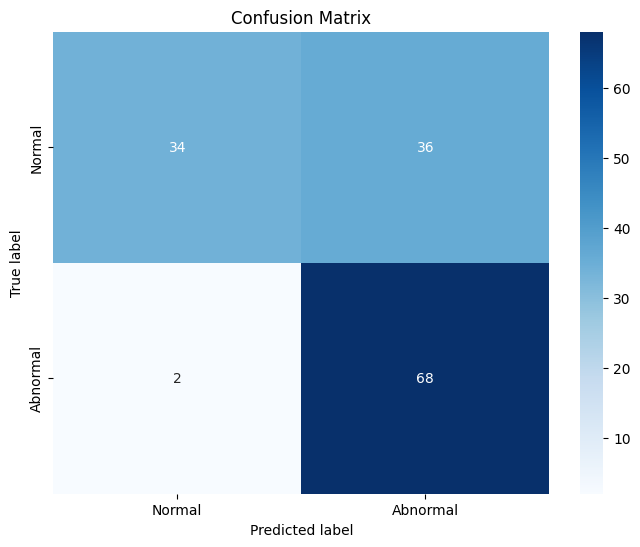
\includegraphics[width=1\linewidth]{Rohit_Master_Thesis//Images/dfm_densenet_best_confusion_matrix.png}
    \caption{Confusion matrix for the best performing configuration for \gls{dfm} model with DenseNet169 backbone, its accuracy is 72.86\%}
    \label{fig:dfm densenet169 confusion matrix}
\end{figure}

After getting good results with the configuration explained above, we thought of checking another variation of the DenseNet169 backbone while keeping the feature extraction layer and scoring type the same as before but using a higher \gls{pca} level of 0.995, allowing for a greater variance in the data. However, the results were more or less similar to the previous configuration, with a slightly lower \gls{auroc} of 0.7190 and an accuracy of 72.14\%, along with a precision of 0.6422 and an F1-score of 0.7821. The recall remained at 1.0, but the decrease in precision compared to the previous configuration indicates that the increased retained variance caused the model to classify a higher number of normal images as anomalous. Finally, DenseNet201 was also tested with the same feature extraction layer, keeping the other hyperparameters the same. This configuration also gave similar results to previous ones highlighted in the table \ref{tab:dfm densenet results}.


% In discussions explain also the difference between scoring type fre and nll
% In discussion also discuss why was the recall for most part 1.0

\subsection*{\gls{dfkde}}

Here, we discuss the results obtained for the model \gls{dfkde}. It combines the power of \gls{dl} with statistical methods like \gls{pca} and \gls{kde}. The model first extracts robust features using a pre-trained deep neural network, then reduces their dimensionality by using \gls{pca}, and finally applying \gls{kde} to model the distribution of normal data. Two backbones were tested in this experiment, namely ResNet18 and Wide-ResNet50. The overview of the results for different configurations in the form of a bar chart is shown in figure \ref{fig:dfkde model results}.

\begin{figure}[ht!]
    \centering
    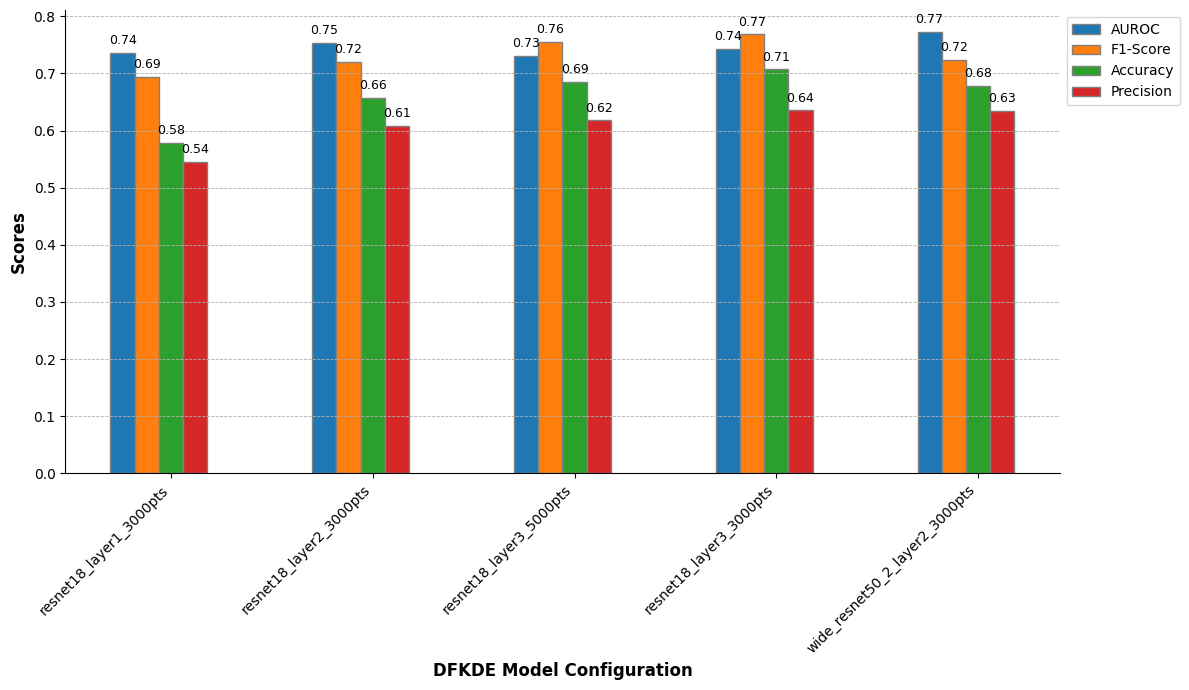
\includegraphics[width=1.2\linewidth]{Rohit_Master_Thesis//Images/dfkde_model_results.png}
    \caption{DFKDE model results for different backbones. The values shown here include \gls{auroc} score, F1-score, accuracy, and precision.}
    \label{fig:dfkde model results}
\end{figure}

\subsubsection*{ResNet18}

For the first experiment with the ResNet18 backbone, we use the feature extraction layer 1. This configuration aims at capturing the lower-level basic features and is trained with a maximum of 3000 training points to fit the \gls{kde} model.

Its results are shown in the table \ref{tab:dfkde resnet18 results}. As can be seen, the performance is not quite good, with \gls{auroc} score of 0.7364 and an accuracy of 57.86\%. Precision is quite low at 0.5447, while recall is high at 0.9571, resulting in an F1-score of 0.6943. The lower precision value indicates that the features extracted from the lower layer lead to the introduction of noise, leading to higher false positives. While the high recall value suggests that the model was still able to detect most of the anomalies correctly. However, the overall performance of the model still suffered as low-level features are less effective in anomaly detection for \gls{dfkde} model.

\begin{table}[ht!]
    \centering
    \begin{tabular}{|l|c|c|c|c|c|c|}
        \hline
        \textbf{Configuration} & \textbf{AUROC} & \textbf{Accuracy(\%)} & \textbf{Precision} & \textbf{Recall} & \textbf{F1-Score} \\ \hline
        Layer1, max training points 3000 & 0.7364 & 57.86\% & 0.5447 & 0.9571 & 0.6943 \\ \hline
        Layer2, max training points 3000 & 0.7535 & 65.71\% & 0.6078 & 0.8857 & 0.7209 \\ \hline
        Layer3, max training points 3000 & 0.7428 & 70.71\% & 0.6355 & 0.9714 & 0.7684 \\ \hline
        Layer3, max training points 5000 & 0.7310 & 68.57\% & 0.6182 & 0.9714 & 0.7556 \\ \hline
    \end{tabular}
    \caption{Results for DFKDE Model with ResNet18 Backbone}
    \label{tab:dfkde resnet18 results}
\end{table}

For the second experiment with the ResNet18 backbone, we used feature extraction layer 2, and the number of maximum data points for \gls{kde} model remained the same as before at 3000.

The model achieved an \gls{auroc} score of 0.7535, which is slightly better than when features were extracted from layer 1, an accuracy of 65,71\% is observed, which is about 14\% higher than that of configuration 1, as can be seen in the table \ref{tab:dfkde resnet18 results}. A precision of 0.6078 and a recall of 0.8857, resulting in an F1-score of 0.7209. This improvement in \gls{auroc} score and precision indicates that the mid-level features are more effective in anomaly detection for \gls{dfkde} model as they maintain the balance of the low-level details and high-level semantic information. Even though recall is slightly reduced compared to layer 1, the improvement in precision indicates a reduction in false positives.

For the third experiment, we select layer 3 for feature extraction of the backbone ResNet18, which is responsible for capturing higher-level semantic information. This layer offers a more abstract representation of the input data, which can be particularly suitable for anomaly detection tasks. This configuration was the best performing one in the \gls{dfkde} model.

As shown in the table \ref{tab:dfkde resnet18 results} an \gls{auroc} score of 0.7427, an accuracy of 70.71\% which is more than 22\% higher than configuration 1, and more than 7\% higher than configuration 2. A further improvement in precision was observed at 0.6355, and a recall of 0.9714, leading to an F1-score of 0.7684. The layer 3 features give more abstract representations of the data, which helped reduce false positive rates further while also maintaining high recall. However, a slight dip in \gls{auroc} compared to layer2 configuration can indicate that while the high-level features are useful, they might lack some of the finer details necessary for achieving good anomaly detection performance.

Next, for the fourth experiment, to examine the effects of increasing the number of training points, we increased the max training points parameter to 5000 points to fit the \gls{kde} model while keeping the backbone and the feature extraction layer the same as ResNet18 layer3. The goal was to see if more training data would improve \gls{kde}'s ability to model normal distribution, as layer 3 gave the best results.

In table \ref{tab:dfkde resnet18 results}, we can see that the model reached an \gls{auroc} score of 0.7310, with an accuracy of 68.57\%, which is lower than the third experiment, and with precision and recall of 0.6182 and 0.9714 respectively, leading to an F1-score of 0.7556. The performance was slightly worse than that of configuration 3, where layer 3 with 3000 max training points was used. This indicates that the number of training points may be less important than the layer from which the features are extracted, at least beyond a threshold.

\subsubsection*{Wide-ResNet50}

The second backbone we experimented with was Wide-ResNet50-2, which is a wider version of the standard ResNet50 architecture. In this experiment, features were extracted using layer 2 of the backbone. This configuration was chosen because the middle layer performed better for the ResNet18 backbone experiments and with the wider architecture, which can capture more detailed feature representations, which could possibly improve the anomaly detection performance.

\begin{table}[ht!]
    \centering
    \begin{tabular}{|l|c|c|c|c|c|c|}
        \hline
        \textbf{Configuration} & \textbf{AUROC} & \textbf{Accuracy(\%)} & \textbf{Precision} & \textbf{Recall} & \textbf{F1-Score} \\ \hline
        Layer2, max training points 3000 & 0.7725 & 67.86\% & 0.6344 & 0.8429 & 0.7239 \\ \hline
    \end{tabular}
    \caption{Results for DFKDE Model with Wide-ResNet50-2 Backbone}
    \label{tab:dfkde wide-resnet50 results}
\end{table}


This configuration showed improved performance in \gls{auroc} score and precision as seen from the table \ref{tab:dfkde wide-resnet50 results} of 0.7725 and 0.6344, respectively. The accuracy was 67.86\%, and the recall fell to 0.8429, resulting in the F1-score of 0.7239. The wider architecture and mid-level features from layer 2 did help the model capture more subtle patterns in the data, which resulted in a higher \gls{auroc} score when compared to ResNet18 experiments. The precision also slightly improved, indicating that the model was comparatively more accurate in detecting true anomalies. However, the lowest recall value of all the experiments combined from resNet18 and Wide-ResNet50 indicates that the model became slightly less sensitive to anomalies, likely as a result of the increase in specificity brought by the wider backbone.

\subsection*{FastFlow}

For this experiment, we used the FastFlow model with ResNet18, Wide-ResNet50-2, \gls{deit}, \gls{cait} as backbones for feature extraction. An overview of all the results is shown in the form of a bar chart in the figure \ref{fig:fastflow model results}. The best performing configuration in terms of accuracy was the one where \gls{deit} architecture was used for feature extraction, achieving 66.87\%. Below, we will discuss all the experiments and their results in detail, grouped based on the backbones used. Here, all the models were trained for 50 epochs except for when callback functionality was used. Then, it is trained until a condition is met.

\begin{figure}[H]
    \centering
    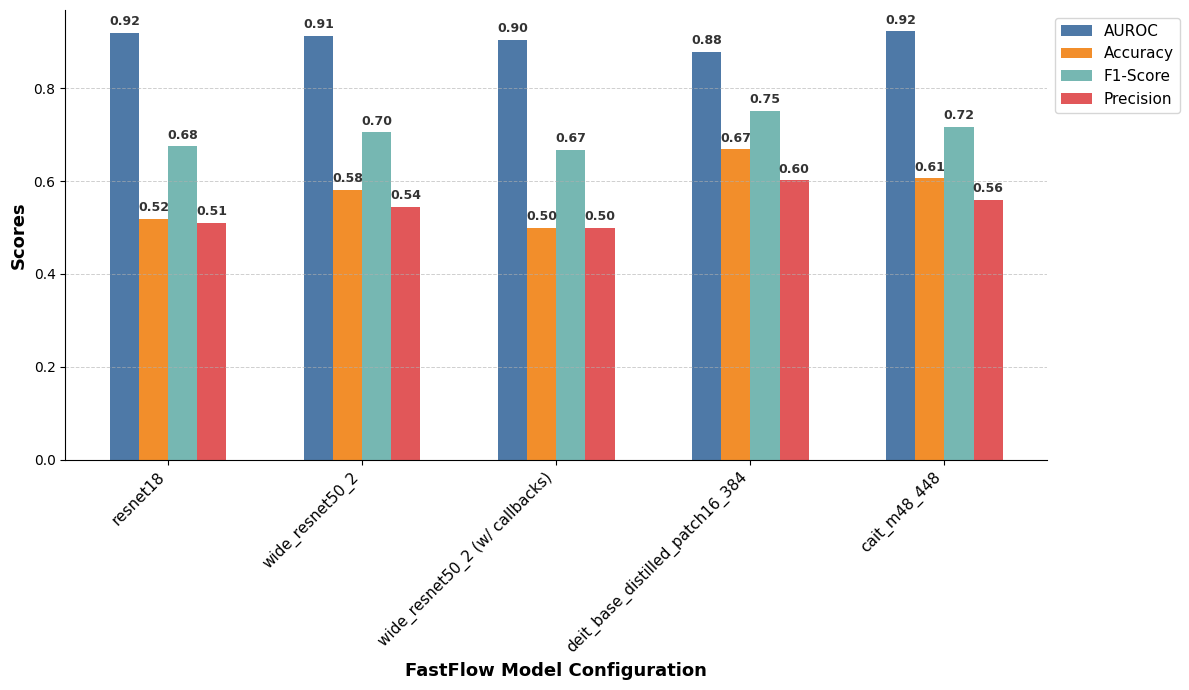
\includegraphics[width=1.2\linewidth]{Rohit_Master_Thesis//Images/fastflow_model_results.png}
    \caption{FastFlow model's results bar-chart for different configurations and backbones used for feature extraction.}
    \label{fig:fastflow model results}
\end{figure}

\subsubsection*{ResNet18}

For the first experiment, we have used ResNet18 as the backbone for feature extraction. This configuration achieved an \gls{auroc} score of 0.9199, which is quite good, and it demonstrates the models effectiveness in distinguishing normal images from abnormal ones on training and testing dataset. But, the overall accuracy on the unseen custom dataset is as good as random guessing, equating to 51.88\%, reflecting imbalanced classification performance, as shown in the table \ref{tab:fastflow resnet18}. The recall of 1.0 shows that the model was able to detect all anomalous instances. However, the precision was low, at 0.5096, giving an F1 score of 0.6751. 

\begin{table}[ht!]
    \centering
    \begin{tabular}{|l|c|c|c|c|c|}
        \hline
        \textbf{Backbone} & \textbf{Accuracy (\%)} & \textbf{AUROC} & \textbf{Precision} & \textbf{Recall} & \textbf{F1-Score} \\ \hline
        ResNet18 & 51.88\% & 0.9199 & 0.5096 & 1.0 & 0.6751 \\ \hline
    \end{tabular}
    \caption{Results for FastFlow model with ResNet18 Backbone}
    \label{tab:fastflow resnet18}
\end{table}

The confusion matrix results show that out of 80 normal samples, only 3 were correctly classified, while 77 were misclassified as abnormal. This significant misclassification of normal samples can be due to simplicity of the ResNet18 architecture, which might lack the depth required to capture subtle differences between normal and anomalous features correctly. Due to this, the model's ability to generalize across the dataset declined, showing its bias toward identifying anomalies but at the cost of higher false positives.

\subsubsection*{Wide-ResNet50}

For the second experiment, we used Wide-ResNet50-2 backbone for feature extraction. Along with that, we employed a callback mechanism. Here, we used early stopping, which monitors the image\_AUROC while training, and when it stays the same for five consecutive epochs, then the training stops and those weights are saved. As can be seen in the table \ref{tab:fastflow wideresnet50}, the \gls{auroc} score dropped slightly to 0.9041 but again achieved 1.0 recall, indicating it was able to classify all the anomalous images correctly. However, the accuracy remained at 50\%, which means the model effectively did not learn anything and is just making random guesses. The precision was 0.5, resulting in an F1-score of 0.666.

The confusion matrix results show that the performance was terrible, as the model classified all the images, whether normal or abnormal, as abnormal.

\begin{table}[ht!]
    \centering
    \begin{tabular}{|l|c|c|c|c|c|}
        \hline
        \textbf{Backbone} & \textbf{Accuracy (\%)} & \textbf{AUROC} & \textbf{Precision} & \textbf{Recall} & \textbf{F1-Score} \\ \hline
        Wide-ResNet50-2 (with callbacks) & 50.00\% & 0.9041 & 0.5000 & 1.0 & 0.6667 \\ \hline
        Wide-ResNet50-2 & 58.13\% & 0.9125 & 0.5442 & 1.0 & 0.7048 \\ \hline
    \end{tabular}
    \caption{Results for FastFlow with Wide-ResNet50-2 Backbone}
    \label{tab:fastflow wideresnet50}
\end{table}

Looking at the above results, we decided to see the effect on the FastFlow model by keeping all the hyperparameters the same but removing the callback mechanism and letting the training continue for 50 epochs. The \gls{auroc} score increased to 0.9125, suggesting that the model's longer training led to better feature extraction. Along with that, the accuracy improved to 58.13\%, with precision reaching 0.5442 and recall of 1.0, resulting in an F1 score of 0.7048.

The results of the confusion matrix showed improvement as well. The number of correctly classified normal samples increased to 13. However, 67 normal samples were still misclassified as abnormal. This suggests that longer training helps the model differentiate between normal and anomalous samples better. This performance improvement can also be due to the backbone's ability to capture more better features over a longer training period, refining the normalizing flow process and providing a more detailed understanding of normality in the dataset. Further, the increase in epochs did not show much improvement from then on.

\subsubsection*{\gls{deit}\_base}

For the fourth experiment, the "\gls{deit} Base Distilled Patch16\_384" backbone was used for feature extraction, and the model was trained for 50 epochs. This configuration resulted in an \gls{auroc} of 0.8787, which is slightly lower than the previous experiments. However, despite that, the model achieved the highest accuracy for the FastFlow model, at 66.88\%. With a precision and recall of 0.6015 and 1.0, respectively, resulting in an F1 score of 0.7512 which is also the highest in all the experiments, as shown in the table \ref{tab:fastflow deit-base}.

\begin{table}[ht!]
    \centering
    \begin{tabular}{|l|c|c|c|c|c|}
        \hline
        \textbf{Backbone} & \textbf{Accuracy (\%)} & \textbf{AUROC} & \textbf{Precision} & \textbf{Recall} & \textbf{F1-Score} \\ \hline
        DeiT Base Distilled Patch16 384 & 66.88\% & 0.8787 & 0.6015 & 1.0 & 0.7512 \\ \hline
    \end{tabular}
    \caption{Results for FastFlow with DeiT\_Base Backbone}
    \label{tab:fastflow deit-base}
\end{table}

The confusion matrix results show that 27 normal images were correctly classified, with 53 being misclassified as abnormal, reflecting its improved performance in detecting normal images compared to earlier configurations. The transformer-based \gls{deit} backbone most likely contributed to these results, as its global attention mechanism enables the model to capture more contextual information across images. However, the slight drop in \gls{auroc} suggests that, while the model is capable of extracting features from normal samples, it might struggle more with identifying anomalies, which can be more subtle and context-dependent.

\subsubsection*{\gls{cait}}

For the fifth and final experiment, the "CaiT-M48" backbone was used and trained for 50 epochs. As can be seen from the table \ref{tab:fastflow cait}, this model achieved the highest image AUROC across all configurations, at 0.9223. The accuracy was 60.63\%, which is about 9\% lower than the configuration with \gls{deit} as the backbone, with a precision of 0.5594 and an F1 score of 0.7175.

\begin{table}[ht!]
    \centering
    \begin{tabular}{|l|c|c|c|c|c|}
        \hline
        \textbf{Backbone} & \textbf{Accuracy (\%)} & \textbf{AUROC} & \textbf{Precision} & \textbf{Recall} & \textbf{F1-Score} \\ \hline
        CaiT M48 448 & 60.63\% & 0.9223 & 0.5594 & 1.0 & 0.7175 \\ \hline
    \end{tabular}
    \caption{Results for FastFlow with CaiT\_M48\_448 Backbone}
    \label{tab:fastflow cait}
\end{table}

The confusion matrix results showed that 17 normal images were correctly classified, while 63 were misclassified as abnormal. Despite no improvement in accuracy over the \gls{deit} configuration results, the \gls{cait} backbone performed better at maintaining a balance between precision and recall.

\subsection*{EfficientAD : }

EfficientAD is a novel approach to visual anomaly detection, specifically developed to operate at millisecond-level latencies. This model was introduced as a lightweight alternative to existing anomaly detection architectures. EfficientAD is built on a \gls{s-t} framework, where the teacher model learns representations from a more complex and larger model while the student attempts to mimic the teacher's performance using fewer resources.

\begin{figure}[ht!]
    \centering
    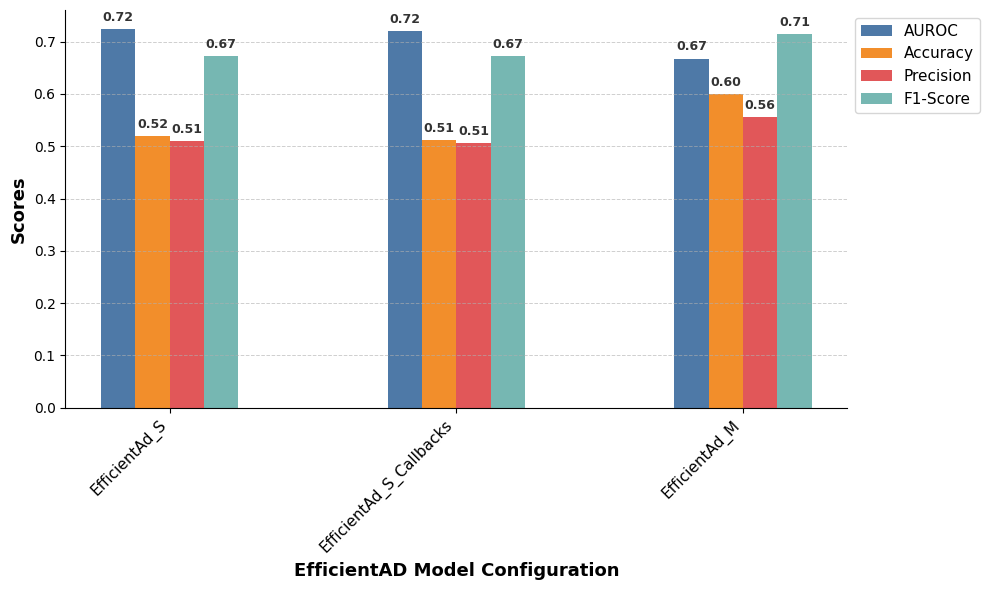
\includegraphics[width=1.2\linewidth]{Rohit_Master_Thesis//Images/efficientad_model_results.png}
    \caption{EfficientAD models result in bar-chart for different configurations used.}
    \label{fig:efficientad model results}
\end{figure}

While the EfficientAD model claims to outperform existing models, such as PatchCore\cite{roth2022totalrecallindustrialanomaly}, as given in the paper \cite{batzner2024efficientadaccuratevisualanomaly}, the experimental results conducted in this study suggest otherwise. The performance of EfficientAD was found to be suboptimal when evaluated on unseen data, as can be seen in the diagram \ref{fig:efficientad model results}. This section will discuss the results of different configurations in detail.

These experiments were carried out using three different configurations of the EfficientAD model. There are two sizes available for the model, which are EfficientAD\_S(small) and EfficientAD\_M(medium). The model size was constant for the first two configurations, but a callback mechanism was added in the second configuration. The Performance metrics used are the same as the rest of the models, namely \gls{auroc}, accuracy, precision, recall, and F1-score. Also, confusion matrices were generated to provide visual insights into how well the model performed in terms of classification.

In the first configuration, the base model (EfficientAdModelSize.S) was used without callbacks, as shown in the table \ref{tab:efficientad results}. This gave the \gls{auroc} of 0.7244. However, the model's accuracy was only 51.87\%, which clearly highlights its struggles in correctly classifying the majority of images. More specifically, out of 80 normal images, only 4 were correctly classified, with the remaining 76 being classified as abnormal, i.e., false positives. But on the other hand, the model performed quite well in detecting abnormal instances, with 79 out of 80 correctly classified as abnormal, resulting in a recall of 0.9875. But the precision is quite low at 0.5097, showing the imbalance between the true positives and false positives. The resulting F1-score was 0.6723, indicating a tendency towards recall, with the model detecting most anomalies but at the cost of misclassifying a large number of normal images as abnormal. Here, all the models were trained for 50 epochs except for when callbacks functionality is used. Then, it is trained until a condition is met.

\begin{table}[ht!]
    \centering
    \begin{tabular}{|l|c|c|c|c|c|}
        \hline
        \textbf{Model Size} & \textbf{AUROC} & \textbf{Accuracy(\%)} & \textbf{Precision} & \textbf{Recall} & \textbf{F1-Score} \\ \hline
        EfficientAd-S & 0.7244 & 51.88\% & 0.5097 & 0.9875 & 0.6723 \\ \hline
        EfficientAd-S (with callbacks) & 0.7203 & 51.25\% & 0.5063 & 1.0 & 0.6723 \\ \hline
        EfficientAd-M & 0.6678 & 60\% & 0.5556 & 1.0 & 0.7143 \\ \hline
    \end{tabular}
    \caption{Performance of EfficientAD Models with Different Sizes}
    \label{tab:efficientad results}
\end{table}

For the second configuration, the same model size (EfficientAdModelSize.S) was used, but ModelCheckpoint and EarlyStopping callbacks were added. The purpose of these callbacks was to improve the training process by ensuring that the model did not overfit and preserving the best weights during the training. Despite these improvements, the model's \gls{auroc} dropped slightly to 0.7203, and an overall accuracy of which relatively remained the same as before at 51.25\%, as seen in the table \ref{tab:efficientad results}. This result suggests that the callbacks had minimal to no impact on the model's ability to generalize on unseen data. In terms of precision and recall, the scores were 0.5063 and 1.0, respectively, this shows us that while the model was able to classify all the abnormal images correctly, but it struggled a lot at classifying the normal images correctly and ended up with lots of false positives. The confusion matrix values further confirm these findings, with only 2 normal samples being correctly classified, with the rest, 78 being misclassified as abnormal. The F1-score came out to be 0.6723, which is identical to that of the first configuration with no callbacks.

In the third and final configuration, the larger variant of the model (EfficientAdModelSize.M) was used. An \gls{auroc} score of 0.6678 was observed, which is less than the smaller model configurations scores, indicating a further decline in the model's ability to differentiate between normal and abnormal instances. Even then, an increase in overall accuracy was observed at 60\% with 16 normal samples correctly classified as normal, with 64 still being misclassified as shown in the confusion matrix \ref{fig:efficientad confusion matrix}. Although this is an improvement compared to other configurations, the model still struggles with a high number of false positives. The recall of 1.0 and increased precision of 0.5556 indicate an improved ability to correctly classify more normal images. The resulting F1-score is 0.7143, which is an improvement over smaller models, but it is still far from ideal.

\begin{figure}[H]
    \centering
    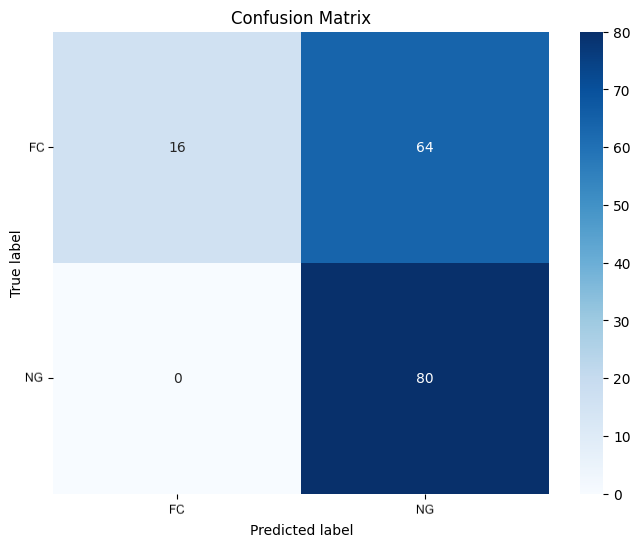
\includegraphics[width=1\linewidth]{Rohit_Master_Thesis//Images/efficientad_confusion_matrix_best.png}
    \caption{Confusion matrix for the best performing configuration for EfficientAD model with size EfficientAdModelSize.M, its accuracy is 60\%}
    \label{fig:efficientad confusion matrix}
\end{figure}




%\subsection{Layer wise performance comparison}

%\subsection{Performance on NG images}

%\subsection{Performance on FC images}

%\subsection{Discussion}

%5.2 The Case for Unsupervised Models: Patchcore's Robustness

%Patchcore emerged as the strongest unsupervised model, achieving 91.25% accuracy and an AUROC of 0.9271. One of the key strengths of Patchcore is its ability to function effectively without requiring labeled anomaly data, making it highly suitable for real-world industrial applications. This model leverages feature representations from multiple layers of the network (layer1 and layer2 in its best configuration), allowing it to capture complex anomalies across different scales and granularities.

%Patchcore's F1 score of 0.9434 further underscores its effectiveness in balancing precision and recall, ensuring that false positives and false negatives are minimized. From a practical standpoint, this makes Patchcore a strong candidate for use in settings where it is crucial to minimize missed anomalies (false negatives) but also to reduce the burden of excessive false positives, which can lead to unnecessary inspections or interventions.

%Additionally, Patchcore's confusion matrix reflects a well-rounded performance with only 2 false negatives and 12 false positives, highlighting its ability to handle both normal and abnormal cases effectively. This is especially important in applications such as predictive maintenance, where the cost of missing a potential failure is high, and unnecessary repairs due to false positives can also be costly.

%Conclusion: Patchcore's robust performance without the need for labeled data makes it an ideal choice for unsupervised anomaly detection tasks, especially in industries like manufacturing, medical diagnostics, and predictive maintenance, where labeling anomalies is often impractical.

% In discussions explain also the difference between scoring type fre and nll
% In discussion also discuss why was the recall for most part 1.0

%Probably for discussion section(remember to paraphrase)
%Explanation of Results

%YOLOv8-M strikes a balance between computational efficiency and accuracy. The model achieves 93.75\% accuracy, which is competitive given its smaller architecture compared to YOLOv8-L. The slightly lower performance is expected due to YOLOv8-M’s reduced depth and number of parameters, which limits its ability to capture as many intricate patterns in the data as YOLOv8-L. However, YOLOv8-M’s simpler structure makes it faster and more computationally efficient, making it suitable for tasks where real-time performance and resource limitations are important.

%Model Comparison and Insights
%YOLOv8-L outperforms YOLOv8-M by achieving 95\% accuracy, compared to YOLOv8-M’s 93.75\%. This difference in performance can be attributed to the larger number of layers and parameters in YOLOv8-L, which allows it to capture more detailed features from the dataset. YOLOv8-L’s larger architecture is particularly beneficial for classification tasks that involve complex patterns or subtle differences between classes, making it a better choice for applications where accuracy is critical.

%However, YOLOv8-M offers significant advantages in terms of speed and computational efficiency. Despite having fewer layers, YOLOv8-M achieves strong results, making it a good option for scenarios where real-time inference is necessary or where computational resources are limited. The slight trade-off in accuracy is reasonable given the gains in efficiency, making YOLOv8-M ideal for environments where fast processing is prioritized over achieving the highest possible accuracy.

%Probably for discussion section(remember to paraphrase)
%Explanation of Results
%The performance of YOLOv8-L is in line with its design as a larger, more powerful model. The depth and complexity of the YOLOv8-L architecture allow it to capture a wide variety of patterns and features in the data, leading to its high precision and recall. The non-maximum suppression (NMS) technique used in YOLOv8 helps further refine the predictions by ensuring that overlapping bounding boxes are filtered, resulting in more accurate object classification. Additionally, YOLOv8-L's anchor-free detection mechanism improves its ability to generalize across objects of various sizes, contributing to its robustness in detecting NG and FC items.


% In DFM resnet results why changing the PCA_level and scoring type to fre resulted in better results?

%Discussion of Results and Insights for DFM

%The results of the experiments provide valuable insights into how the choice of backbone network, feature extraction layer, and scoring method influence the performance of the DFM model. Across all configurations, the model demonstrated high recall values, indicating its strong ability to detect anomalous samples. However, the key challenge in most configurations was improving precision, as many configurations suffered from high false-positive rates. This imbalance between precision and recall was most noticeable in configurations that used higher-level feature layers, such as layer4 in ResNet50, which may have caused the model to focus on abstract features less relevant for anomaly detection.

%The use of PCA for dimensionality reduction also played a crucial role in balancing the model’s performance. A PCA level of 0.97 generally provided a good balance between computational efficiency and information retention, while increasing the PCA level to 0.995 resulted in slightly higher overfitting and a decrease in precision. Additionally, the frequentist score type consistently outperformed the negative log-likelihood score in anomaly detection tasks, as it provided a more robust measure of the distance between the new data points and the normal data distribution.

%In conclusion, the DFM model’s performance varied significantly across different configurations. The best-performing setup used DenseNet169 with features extracted from DenseBlock3, a PCA level of 0.97, and the frequentist score type, achieving a balance between high precision and recall while maintaining a high sensitivity to anomalies. Future work could explore the integration of attention mechanisms or ensemble methods to further improve precision and reduce the false-positive rate, particularly in configurations that show a tendency to misclassify normal samples as anomalies.

%I can add diagram showing the performance according to layers

%DFKDE

%Discussion of Results Based on Backbone
%The results of the experiments show that the choice of backbone architecture and the layer from which features are extracted significantly affect the performance of the DFKDE model. Across the ResNet18 experiments, the best results were obtained when extracting features from layer2 or layer3, as these layers provided a balance between precision and recall. Layer1, which captures low-level features, produced the lowest precision and accuracy, likely due to its inability to capture the necessary high-level patterns required for accurate anomaly detection.

%In contrast, the Wide-ResNet50-2 backbone consistently outperformed ResNet18 in terms of AUROC, suggesting that the wider architecture was more effective at capturing subtle differences between normal and anomalous data. However, the performance of the Wide-ResNet50-2 model was highly dependent on the number of principal components retained during the PCA step. Retaining too many components, as seen in the final experiment, introduced noise that reduced precision, while using fewer components provided a better balance between recall and precision.

%In conclusion, the DFKDE model's performance is sensitive to both the choice of backbone architecture and the feature extraction layer. While ResNet18 provides satisfactory results, Wide-ResNet50-2 offers better overall performance, especially when mid-level features are extracted from layer2. The trade-off between precision and recall is heavily influenced by the layer used for feature extraction, and careful tuning of the PCA level is essential for optimizing the model’s anomaly detection capabilities. These findings suggest that DFKDE is a flexible and powerful anomaly detection framework, with its performance closely tied to the choices made during the feature extraction and dimensionality reduction processes.

%EfficientAD Discussion
%The results of the experiments demonstrate that while EfficientAD is designed for efficiency, it struggles with the accuracy and precision required for real-world anomaly detection tasks. In all three configurations, the model exhibited high recall, meaning that it was consistently able to identify abnormal instances. This is an important quality for anomaly detection, particularly in applications where it is critical to catch every possible anomaly. However, the model’s precision was consistently low across all configurations, highlighting a major issue: a significant number of normal samples were misclassified as anomalies.

%One of the key reasons for this performance discrepancy could be the model's underlying architecture. EfficientAD's focus on reducing computational complexity through the use of a smaller student model might have come at the cost of reduced representational capacity. The model's teacher-student framework is designed to ensure that the student model can mimic the teacher’s outputs, but this transfer of knowledge might not be as effective when it comes to detecting subtle variations between normal and abnormal instances. In contrast, PatchCore, which relies on more robust and larger feature representations, seems to be better suited for capturing these nuances, which could explain why it outperformed EfficientAD in these experiments.

%Another factor to consider is the dataset used in these experiments. While EfficientAD was trained and tested on a large-scale dataset like Imagenet, the generalization capabilities of the model may be limited when applied to unseen data. Anomaly detection is highly sensitive to the specific characteristics of the dataset, and a model that performs well on one dataset may not necessarily generalize to others. In this case, the dataset used for testing may contain subtle differences from the training data, which EfficientAD was unable to capture, leading to a higher rate of misclassification.

%PatchCore’s superior performance can also be attributed to its underlying architectural advantages. PatchCore uses a memory bank of features extracted from the training data, which allows it to compare new samples against a more diverse and representative set of normal instances. This approach enables PatchCore to better detect subtle anomalies that might be overlooked by more simplified models like EfficientAD. In contrast, EfficientAD’s reliance on a student-teacher framework, while computationally efficient, may result in the loss of critical information that is necessary for accurate anomaly detection.

%Additionally, PatchCore’s design allows for better feature extraction, as it does not reduce the complexity of the model as much as EfficientAD. This could explain why, despite being an older model, PatchCore consistently outperforms EfficientAD in terms of both precision and recall. EfficientAD's strength lies in its ability to operate in real-time and on resource-constrained devices, but this efficiency comes with trade-offs in accuracy that may not be acceptable for certain applications.

%In conclusion, while EfficientAD offers an attractive solution for real-time anomaly detection in resource-constrained environments, it faces significant challenges in achieving the level of accuracy and precision required for high-stakes applications. The model’s high recall is commendable, but its low precision indicates that it generates too many false positives, which could limit its usability in certain domains. PatchCore, on the other hand, continues to outperform newer models like EfficientAD due to its more robust feature extraction and memory-based approach. As such, the choice between EfficientAD and PatchCore ultimately depends on the specific requirements of the application, with EfficientAD being more suited for real-time tasks where speed is of the essence, and PatchCore being the better choice for tasks where accuracy is paramount.


%Fastflow Discussion and Insights

%Across the experiments, we observe that increasing model complexity through the use of wider or deeper backbones generally improves anomaly detection, though at the cost of classifying normal images less accurately. The backbone architectures like Wide-ResNet50-2, DeiT, and CaiT each offered unique advantages. Wide-ResNet50-2, with its increased width, struggled with balancing normal and anomalous classifications. DeiT, with its transformer-based approach, improved classification of normal samples, and CaiT’s deep attention mechanism allowed for even more nuanced understanding of the image space, reflected by its superior AUROC.

%FastFlow’s reliance on normalizing flows works well in modeling the distribution of normal images but can struggle when anomalies are not sufficiently distinct in the feature space. This is evident from the precision-recall tradeoff seen across all experiments: while recall was consistently high, precision fluctuated, highlighting that misclassifications of normal samples as abnormal remained a challenge.

%Incorporating pre-trained models provided a solid foundation, though the results suggest that the specific nature of anomaly detection tasks may require fine-tuning of these pre-trained backbones for optimal performance. Training for additional epochs, as seen in Experiments 3 through 5, consistently improved results, implying that FastFlow benefits from extended training periods to better capture the feature space of normal images.

%These findings highlight that while FastFlow is effective at detecting anomalies, future work could focus on balancing the precision-recall tradeoff, perhaps through more advanced fine-tuning techniques or hybrid architectures that combine the benefits of convolutional networks and transformers, or more carefully tuned flow step configurations.




\clearpage
\chapter{Discussion}

In this section, we will provide a more deeper understanding of the results. Particularly, we focus on comparing the performance of supervised and unsupervised approaches, also PatchCore's performance relative to the baseline \gls{yolo} model, and to try and examine the reasons behind the underperformance of newer models such as EfficientAD when compared to PatchCore. Also, we will investigate the consistently high recall value observed in most anomaly detection models in our experiments.

\section*{Supervised vs. Unsupervised Learning}

One of the key objectives of this thesis was to evaluate the performance differences between the supervised and unsupervised models for anomaly detection. Supervised learning methods, in our case \gls{yolo}, usually require a large amount of labeled training data. This can be challenging for the \gls{pcb} manufacturing, where defects can be rare, and labeling requires domain experts, which can be time-consuming and expensive. Whereas unsupervised models such as PatchCore, \gls{dfm}, and EfficientAD use patterns from normal data to identify anomalies, which reduces the dependency on labeled datasets. \textbf{In anomaly detection, unsupervised learning means that the model is trained only on normal data, allowing it to learn the features of normal data and flag any deviations from it as anomalies. Even though the model is only exposed to normal samples during training, it does not have access to labeled information about defects or a mask indicating their location, which is required during supervised training methods. This makes it unsupervised as the model is not explicitly taught where defects are but instead learns to detect anomalies from normal patterns on its own.} The results also demonstrate that despite having no information about the defect location, it can still perform quite well, with PatchCore reaching an accuracy of 91.25\%, which is quite good when compared to the baseline \gls{yolo}v8-m with only 2.5\% difference in their accuracy. These results show the effectiveness of unsupervised learning models, which can also come close to the performance of supervised models.

\section*{Performance of PatchCore vs Baseline \gls{yolo}}

The PatchCore model achieved an accuracy of 91.25\%, showing its effectiveness in anomaly detection. While \gls{yolo}v8-M and \gls{yolo}v8-L achieved higher overall accuracy scores of 93.75\% and 95\%, respectively, \gls{yolo} models showed better results in most aspects, particularly in achieving fewer false positives, as evident from their confusion matrices. \textbf{PatchCore, however, provided a competitive approach}, particularly in its unique patch-level analysis. Unlike \gls{yolo}, which processes the entire image, PatchCore analyzes smaller patches of an image, which can be advantageous in certain scenarios. Despite this, the \gls{yolo} models generally outperformed PatchCore.

PatchCore's results are significant in addressing the 'cold start' problem, which refers to the lack of anomalous samples during training. By leveraging only normal data, \textbf{PatchCore provides a competitive alternative approach for industrial defect detection, successfully detecting anomalies without needing extensive labeled defect data like in supervised learning approaches}. This characteristic makes PatchCore suitable for quality assurance in high-volume production environments, where the ability to detect rare faults with minimal labeled data is crucial. Additionally, since no extensive manual labeling is required, this approach can help in significantly reducing costs.

%\section*{Why Newer Models couldn't Outperform PatchCore}
\section*{Limitations of Newer Models}

Although models like EfficientAD and FastFlow are more recent, with specific strengths, such as computational efficiency and speed, they still could not surpass PatchCore's performance in terms of accuracy. There could be several reasons for this outcome. Firstly, PatchCore's dependency on memory banks of patch-level features allows for a rich representation of normal patterns, which facilitates robust anomaly detection. The coreset subsampling method used in PatchCore reduces redundancy in the feature space, which helps improving it's efficiency when comparing new data with the stored nominal patches.

In contrast, even though EfficientAD is computationally efficient and fast due to its \gls{s-t} network structure, it lacks the detailed patch-level comparison that PatchCore employs. EfficientAD focuses on lightweight architectures that excel in computational efficiency, but this can often come at the cost of the deep representational power needed to identify subtle anomalies in complex datasets. Similarly, \gls{dfm} relies on probabilistic modeling of deep features. However, it lacks the fine granularity offered by PatchCore's patch-wise anomaly scoring, making it less effective when dealing with highly localized defects. FastFlow, which uses normalizing flows, also struggled to outperform PatchCore due to its limited ability to capture complex defect patterns. FastFlow's dependence on a more generalized feature extraction approach makes it less capable of identifying complex or subtle anomalies compared to PatchCore's specialized patch-level method.

In order to further highlight the differences in model performance, we compared key metrics such as accuracy, recall, and precision across all the unsupervised models. PatchCore achieved an accuracy of 91.25\%, indicating its strong ability to detect defects. \gls{yolo}v8-M and \gls{yolo}v8-L, while fast and achieving accuracies, showed better results in capturing anomalies with fewer false positives. EfficientAD, with its focus on computational efficiency, demonstrated quick inference times but could not match PatchCore's accuracy, primarily due to its lightweight architecture. \gls{dfm}, which uses probabilistic deep feature modeling, also fell short in accuracy compared to PatchCore, struggling with the complex and diverse nature of the defect patterns. This comparative analysis highlights the trade-offs between computational efficiency and detection accuracy among the different models.

\section*{High Recall in Anomaly Detection Models results}

A notable observation across the evaluated models was the consistent high recall, often reaching 1.0. This behavior can be explained by the nature of anomaly detection tasks, in which the models are generally trained to identify any deviations from the learned distribution of normal data. In many industrial applications, it is crucial to capture all possible defects, even at the risk of producing false positives, to ensure product reliability. This drives the models towards maximizing recall, ensuring that no defective sample is overlooked. High recall is particularly important in situations where the cost of missing a defect is far greater than the cost of examining a false positive.

However, this emphasis on recall may come with the drawback of lower precision, as observed in some models. Precision measures the ability to correctly classify anomalies without misclassifying normal samples, and a lower precision value indicates a higher rate of false positives. In practical terms, while a high recall ensures comprehensive defect coverage, the accompanying lower precision necessitates additional post inspection checks to filter out the false positives.

\section*{Final Thoughts}

While none of the unsupervised learning models could outperform the baseline \gls{yolo} model, but PatchCore still provided competitive results. Its ability to correctly detect anomalies without the need for labeled data or a mask during training makes it a valuable alternative, especially in settings where labeling is costly or impractical. This not only helps reduce the dependency on extensive manual labeling but also significantly cuts down the associated costs, making PatchCore a practical choice for industrial applications. 

\clearpage
\section{Conclusion \& Future Works}
\section{Summary}

%A summary must be included in a master's thesis, as formulated in \cite{FPOMathematik10} Section 34(6).

%The thesis is structured into seven key chapters, they are as mentioned below,

\begin{itemize}
    \item \textbf{Chapter 1: Introduction:} In this chapter, the motivation for improving the efficiency of solder joint inspection in \gls{pcb} manufacturing is introduced. This discussion highlights the limitations of current inspection methods, including manual examination and supervised learning, are discussed, establishing the need for unsupervised learning as a viable alternative to reduce dependency on labeled data.

    \item \textbf{Chapter 2: Theoretical Background:} This chapter lays out the theoretical knowledge required to understand the research. It covers the concepts of supervised and unsupervised image processing, highlighting the advantages of using unsupervised learning for anomaly detection. It also introduces relevant models and techniques, such as convolutional neural networks (CNNs), PatchCore, EfficientAD, etc., used in supervised and unsupervised approaches.

    \item \textbf{Chapter 3: Methods:} The methodology chapter describes the dataset used in this study, which consists of images of solder joints that are either normal or defective. The experimental setup includes training various unsupervised models from the Anomalib library, such as PatchCore, \gls{dfm}, and EfficientAD. The processes for hyperparameter tuning, data preparation, and model evaluation are outlined, along with the metrics used for evaluating model performance.

    \item \textbf{Chapter 4: Results:} This chapter presents the results obtained from evaluating the performance of the different unsupervised models on our dataset. PatchCore emerged as the best-performing model. Comparative analysis of \gls{dfm}, EfficientAD, and other models is also provided, highlighting the strengths and weaknesses of each model in anomaly detection.

    \item \textbf{Chapter 5: Discussion:} The discussion chapter explores the implications of the results, emphasizing the scalability and efficiency of unsupervised methods for anomaly detection in \gls{pcb} manufacturing. Challenges faced during the research, such as the long training times of some models, are also addressed.

    \item \textbf{Chapter 6: Future Works:} This chapter discusses the potential future directions for this research. Suggestions include exploring the use of Vision Transformers for enhanced anomaly detection and optimizing current methods to further reduce training times and improve accuracy. This chapter also highlights the broader applicability of unsupervised learning techniques in other defect detection tasks.

    \item \textbf{Chapter 7: Conclusion:} The conclusion summarizes the key findings, highlighting the benefits of using unsupervised learning for anomaly detection in \gls{pcb} manufacturing. It also highlights how unsupervised models can make the inspection process more scalable and reduce the dependence on manual labeling. This chapter concludes by discussing future research opportunities, including the integration of advanced models like Vision Transformers.
\end{itemize}

\clearpage
%\printglossary[type=\acronymtype, toctitle=Abbreviations]
\printunsrtglossary[type=abbreviations]
%\printglossary[type=abbreviation]


\clearpage
\urlstyle{same}
% Sollen Literaturnachweise eingebunden werden, die nicht zitiert wurden,
% so kann der Befehl \nocite{} verwendet werden.
%\bibliographystyle{plainurl}
% Fuer deutschsprachige Texte fast besser geeignet


%\bibliographystyle{natdin}
\bibliographystyle{unsrtnat}

\bibliography{bibliography}
\addcontentsline{toc}{section}{Bibliography}

% Erklärung 

\clearpage\thispagestyle{empty}



\begin{center}\textbf{\large Declaration}\end{center}

\noindent
 I hereby certify that I have written this thesis independently
and that I have not used any sources or aids other than those indicated,
that all passages of the work which have been taken over verbatim or in spirit from other sources
from other sources have been marked as such and that the work 
has not yet been submitted to any examination authority in the same or a similar form.


\vspace{4\baselineskip}

\noindent
Erlangen, \today \hspace*{2cm} Rohit Potdukhe

% Lebenslauf

%\clearpage
%\pagestyle{empty}


\begin{center}
{\sc \LARGE
CV
}

\medskip

\medskip

{\sc \Large
Myfirstname Mylastname
}

\end{center}

\bigskip
\rule{\textwidth}{0.1em}




\subsection*{\sc Personal data}
\begin{tabular}{lp{9cm}}
Name & Myfirstname Mylastname\\
Born &  Day of birth\\
Adress & street number \\
        & zip code city
\end{tabular}
\smallskip

\rule{\textwidth}{0.1em}



\subsection*{\sc Education}
\begin{tabular}{lp{9cm}}
09/1977 - 08/1981 &  elementary school\\
09/1981 - 06/1990 & high school\\
\end{tabular}

\smallskip
\rule{\textwidth}{0.1em}

\subsection*{\sc Study}
\begin{tabular}{lp{9cm}}
09/1991 - 08/1993 & University X \\
09/1993 - 06/1996 & University Y
\end{tabular}


\smallskip
\rule{\textwidth}{0.1em}


\subsection*{\sc Other activities}
\begin{tabular}{lp{9cm}}
09/1990 - 08/1991 & run up and jump
\end{tabular}


\smallskip
\rule{\textwidth}{0.1em}



%\addcontentsline{toc}{section}{Curriculum Vitae}
\end{document}



